\documentclass[twoside]{book}

% Packages required by doxygen
\usepackage{fixltx2e}
\usepackage{calc}
\usepackage{doxygen}
\usepackage[export]{adjustbox} % also loads graphicx
\usepackage{graphicx}
\usepackage[utf8]{inputenc}
\usepackage{makeidx}
\usepackage{multicol}
\usepackage{multirow}
\PassOptionsToPackage{warn}{textcomp}
\usepackage{textcomp}
\usepackage[nointegrals]{wasysym}
\usepackage[table]{xcolor}

% Font selection
\usepackage[T1]{fontenc}
\usepackage[scaled=.90]{helvet}
\usepackage{courier}
\usepackage{amssymb}
\usepackage{sectsty}
\renewcommand{\familydefault}{\sfdefault}
\allsectionsfont{%
  \fontseries{bc}\selectfont%
  \color{darkgray}%
}
\renewcommand{\DoxyLabelFont}{%
  \fontseries{bc}\selectfont%
  \color{darkgray}%
}
\newcommand{\+}{\discretionary{\mbox{\scriptsize$\hookleftarrow$}}{}{}}

% Page & text layout
\usepackage{geometry}
\geometry{%
  a4paper,%
  top=2.5cm,%
  bottom=2.5cm,%
  left=2.5cm,%
  right=2.5cm%
}
\tolerance=750
\hfuzz=15pt
\hbadness=750
\setlength{\emergencystretch}{15pt}
\setlength{\parindent}{0cm}
\setlength{\parskip}{3ex plus 2ex minus 2ex}
\makeatletter
\renewcommand{\paragraph}{%
  \@startsection{paragraph}{4}{0ex}{-1.0ex}{1.0ex}{%
    \normalfont\normalsize\bfseries\SS@parafont%
  }%
}
\renewcommand{\subparagraph}{%
  \@startsection{subparagraph}{5}{0ex}{-1.0ex}{1.0ex}{%
    \normalfont\normalsize\bfseries\SS@subparafont%
  }%
}
\makeatother

% Headers & footers
\usepackage{fancyhdr}
\pagestyle{fancyplain}
\fancyhead[LE]{\fancyplain{}{\bfseries\thepage}}
\fancyhead[CE]{\fancyplain{}{}}
\fancyhead[RE]{\fancyplain{}{\bfseries\leftmark}}
\fancyhead[LO]{\fancyplain{}{\bfseries\rightmark}}
\fancyhead[CO]{\fancyplain{}{}}
\fancyhead[RO]{\fancyplain{}{\bfseries\thepage}}
\fancyfoot[LE]{\fancyplain{}{}}
\fancyfoot[CE]{\fancyplain{}{}}
\fancyfoot[RE]{\fancyplain{}{\bfseries\scriptsize Generated by Doxygen }}
\fancyfoot[LO]{\fancyplain{}{\bfseries\scriptsize Generated by Doxygen }}
\fancyfoot[CO]{\fancyplain{}{}}
\fancyfoot[RO]{\fancyplain{}{}}
\renewcommand{\footrulewidth}{0.4pt}
\renewcommand{\chaptermark}[1]{%
  \markboth{#1}{}%
}
\renewcommand{\sectionmark}[1]{%
  \markright{\thesection\ #1}%
}

% Indices & bibliography
\usepackage{natbib}
\usepackage[titles]{tocloft}
\setcounter{tocdepth}{3}
\setcounter{secnumdepth}{5}
\makeindex

% Hyperlinks (required, but should be loaded last)
\usepackage{ifpdf}
\ifpdf
  \usepackage[pdftex,pagebackref=true]{hyperref}
\else
  \usepackage[ps2pdf,pagebackref=true]{hyperref}
\fi
\hypersetup{%
  colorlinks=true,%
  linkcolor=blue,%
  citecolor=blue,%
  unicode%
}

% Custom commands
\newcommand{\clearemptydoublepage}{%
  \newpage{\pagestyle{empty}\cleardoublepage}%
}

\usepackage{caption}
\captionsetup{labelsep=space,justification=centering,font={bf},singlelinecheck=off,skip=4pt,position=top}

%===== C O N T E N T S =====

\begin{document}

% Titlepage & ToC
\hypersetup{pageanchor=false,
             bookmarksnumbered=true,
             pdfencoding=unicode
            }
\pagenumbering{alph}
\begin{titlepage}
\vspace*{7cm}
\begin{center}%
{\Large Plant-\/o-\/\+Matic }\\
\vspace*{1cm}
{\large Generated by Doxygen 1.8.13}\\
\end{center}
\end{titlepage}
\clearemptydoublepage
\pagenumbering{roman}
\tableofcontents
\clearemptydoublepage
\pagenumbering{arabic}
\hypersetup{pageanchor=true}

%--- Begin generated contents ---
\chapter{Hierarchical Index}
\section{Class Hierarchy}
This inheritance list is sorted roughly, but not completely, alphabetically\+:\begin{DoxyCompactList}
\item \contentsline{section}{D\+H\+T11}{\pageref{classDHT11}}{}
\item \contentsline{section}{D\+H\+T11callback}{\pageref{classDHT11callback}}{}
\begin{DoxyCompactList}
\item \contentsline{section}{D\+H\+T11\+Sample\+Call\+Back}{\pageref{classDHT11SampleCallBack}}{}
\item \contentsline{section}{D\+H\+T11\+Sample\+Call\+Back}{\pageref{classDHT11SampleCallBack}}{}
\end{DoxyCompactList}
\item \contentsline{section}{J\+S\+O\+N\+C\+G\+I\+Handler\+:\+:G\+E\+T\+Callback}{\pageref{classJSONCGIHandler_1_1GETCallback}}{}
\begin{DoxyCompactList}
\item \contentsline{section}{J\+S\+O\+N\+C\+G\+I\+M\+C\+P3008\+Callback}{\pageref{classJSONCGIMCP3008Callback}}{}
\item \contentsline{section}{J\+S\+O\+N\+D\+H\+T11\+Callback\+Hum}{\pageref{classJSONDHT11CallbackHum}}{}
\item \contentsline{section}{J\+S\+O\+N\+D\+H\+T11\+Callback\+Temp}{\pageref{classJSONDHT11CallbackTemp}}{}
\item \contentsline{section}{J\+S\+O\+N\+Ultra\+Callback}{\pageref{classJSONUltraCallback}}{}
\end{DoxyCompactList}
\item \contentsline{section}{J\+S\+O\+N\+C\+G\+I\+Handler}{\pageref{classJSONCGIHandler}}{}
\item \contentsline{section}{J\+S\+O\+N\+C\+G\+I\+Handler\+:\+:J\+S\+O\+N\+Generator}{\pageref{classJSONCGIHandler_1_1JSONGenerator}}{}
\item \contentsline{section}{M\+C\+P3008}{\pageref{classMCP3008}}{}
\item \contentsline{section}{M\+C\+P3008callback}{\pageref{classMCP3008callback}}{}
\begin{DoxyCompactList}
\item \contentsline{section}{Soil\+Sensor\+Sample\+Call\+Back}{\pageref{classSoilSensorSampleCallBack}}{}
\item \contentsline{section}{Soil\+Sensor\+Sample\+Call\+Back}{\pageref{classSoilSensorSampleCallBack}}{}
\end{DoxyCompactList}
\item \contentsline{section}{J\+S\+O\+N\+C\+G\+I\+Handler\+:\+:P\+O\+S\+T\+Callback}{\pageref{classJSONCGIHandler_1_1POSTCallback}}{}
\item \contentsline{section}{pump}{\pageref{classpump}}{}
\item \contentsline{section}{Ultrasonic}{\pageref{classUltrasonic}}{}
\item \contentsline{section}{Ultrasonic\+Callback}{\pageref{classUltrasonicCallback}}{}
\begin{DoxyCompactList}
\item \contentsline{section}{Ultra\+Sonic\+Sensor\+Sample\+Callback}{\pageref{classUltraSonicSensorSampleCallback}}{}
\item \contentsline{section}{Ultra\+Sonic\+Sensor\+Sample\+Callback}{\pageref{classUltraSonicSensorSampleCallback}}{}
\end{DoxyCompactList}
\end{DoxyCompactList}

\chapter{Data Structure Index}
\section{Data Structures}
Here are the data structures with brief descriptions\+:\begin{DoxyCompactList}
\item\contentsline{section}{\hyperlink{classDHT11}{D\+H\+T11} }{\pageref{classDHT11}}{}
\item\contentsline{section}{\hyperlink{classDHT11callback}{D\+H\+T11callback} }{\pageref{classDHT11callback}}{}
\item\contentsline{section}{\hyperlink{classDHT11SampleCallBack}{D\+H\+T11\+Sample\+Call\+Back} }{\pageref{classDHT11SampleCallBack}}{}
\item\contentsline{section}{\hyperlink{classJSONCGIHandler_1_1GETCallback}{J\+S\+O\+N\+C\+G\+I\+Handler\+::\+G\+E\+T\+Callback} }{\pageref{classJSONCGIHandler_1_1GETCallback}}{}
\item\contentsline{section}{\hyperlink{classJSONCGIHandler}{J\+S\+O\+N\+C\+G\+I\+Handler} }{\pageref{classJSONCGIHandler}}{}
\item\contentsline{section}{\hyperlink{classJSONCGIMCP3008Callback}{J\+S\+O\+N\+C\+G\+I\+M\+C\+P3008\+Callback} }{\pageref{classJSONCGIMCP3008Callback}}{}
\item\contentsline{section}{\hyperlink{classJSONDHT11CallbackHum}{J\+S\+O\+N\+D\+H\+T11\+Callback\+Hum} }{\pageref{classJSONDHT11CallbackHum}}{}
\item\contentsline{section}{\hyperlink{classJSONDHT11CallbackTemp}{J\+S\+O\+N\+D\+H\+T11\+Callback\+Temp} }{\pageref{classJSONDHT11CallbackTemp}}{}
\item\contentsline{section}{\hyperlink{classJSONCGIHandler_1_1JSONGenerator}{J\+S\+O\+N\+C\+G\+I\+Handler\+::\+J\+S\+O\+N\+Generator} }{\pageref{classJSONCGIHandler_1_1JSONGenerator}}{}
\item\contentsline{section}{\hyperlink{classJSONUltraCallback}{J\+S\+O\+N\+Ultra\+Callback} }{\pageref{classJSONUltraCallback}}{}
\item\contentsline{section}{\hyperlink{classMCP3008}{M\+C\+P3008} }{\pageref{classMCP3008}}{}
\item\contentsline{section}{\hyperlink{classMCP3008callback}{M\+C\+P3008callback} }{\pageref{classMCP3008callback}}{}
\item\contentsline{section}{\hyperlink{classJSONCGIHandler_1_1POSTCallback}{J\+S\+O\+N\+C\+G\+I\+Handler\+::\+P\+O\+S\+T\+Callback} }{\pageref{classJSONCGIHandler_1_1POSTCallback}}{}
\item\contentsline{section}{\hyperlink{classpump}{pump} }{\pageref{classpump}}{}
\item\contentsline{section}{\hyperlink{classSoilSensorSampleCallBack}{Soil\+Sensor\+Sample\+Call\+Back} }{\pageref{classSoilSensorSampleCallBack}}{}
\item\contentsline{section}{\hyperlink{classUltrasonic}{Ultrasonic} }{\pageref{classUltrasonic}}{}
\item\contentsline{section}{\hyperlink{classUltrasonicCallback}{Ultrasonic\+Callback} }{\pageref{classUltrasonicCallback}}{}
\item\contentsline{section}{\hyperlink{classUltraSonicSensorSampleCallback}{Ultra\+Sonic\+Sensor\+Sample\+Callback} }{\pageref{classUltraSonicSensorSampleCallback}}{}
\end{DoxyCompactList}

\chapter{File Index}
\section{File List}
Here is a list of all files with brief descriptions\+:\begin{DoxyCompactList}
\item\contentsline{section}{src/\hyperlink{demo_8cpp}{demo.\+cpp} }{\pageref{demo_8cpp}}{}
\item\contentsline{section}{src/\hyperlink{DHT11_8cpp}{D\+H\+T11.\+cpp} }{\pageref{DHT11_8cpp}}{}
\item\contentsline{section}{src/\hyperlink{DHT11_8h}{D\+H\+T11.\+h} }{\pageref{DHT11_8h}}{}
\item\contentsline{section}{src/\hyperlink{dht11__callback_8cpp}{dht11\+\_\+callback.\+cpp} }{\pageref{dht11__callback_8cpp}}{}
\item\contentsline{section}{src/\hyperlink{global__variables_8h}{global\+\_\+variables.\+h} }{\pageref{global__variables_8h}}{}
\item\contentsline{section}{src/\hyperlink{json__fastcgi__web__api_8h}{json\+\_\+fastcgi\+\_\+web\+\_\+api.\+h} }{\pageref{json__fastcgi__web__api_8h}}{}
\item\contentsline{section}{src/\hyperlink{main_8cpp}{main.\+cpp} }{\pageref{main_8cpp}}{}
\item\contentsline{section}{src/\hyperlink{MCP3008_8cpp}{M\+C\+P3008.\+cpp} }{\pageref{MCP3008_8cpp}}{}
\item\contentsline{section}{src/\hyperlink{MCP3008_8h}{M\+C\+P3008.\+h} }{\pageref{MCP3008_8h}}{}
\item\contentsline{section}{src/\hyperlink{pump_8cpp}{pump.\+cpp} }{\pageref{pump_8cpp}}{}
\item\contentsline{section}{src/\hyperlink{pump_8h}{pump.\+h} }{\pageref{pump_8h}}{}
\item\contentsline{section}{src/\hyperlink{soil__callback_8cpp}{soil\+\_\+callback.\+cpp} }{\pageref{soil__callback_8cpp}}{}
\item\contentsline{section}{src/\hyperlink{treshhold_8h}{treshhold.\+h} }{\pageref{treshhold_8h}}{}
\item\contentsline{section}{src/\hyperlink{ultrasonic_8cpp}{ultrasonic.\+cpp} }{\pageref{ultrasonic_8cpp}}{}
\item\contentsline{section}{src/\hyperlink{ultrasonic_8h}{ultrasonic.\+h} }{\pageref{ultrasonic_8h}}{}
\item\contentsline{section}{src/\hyperlink{ultrasonic__callback_8cpp}{ultrasonic\+\_\+callback.\+cpp} }{\pageref{ultrasonic__callback_8cpp}}{}
\end{DoxyCompactList}

\chapter{Data Structure Documentation}
\hypertarget{classDHT11}{}\section{D\+H\+T11 Class Reference}
\label{classDHT11}\index{D\+H\+T11@{D\+H\+T11}}


{\ttfamily \#include $<$D\+H\+T11.\+h$>$}



Collaboration diagram for D\+H\+T11\+:
\nopagebreak
\begin{figure}[H]
\begin{center}
\leavevmode
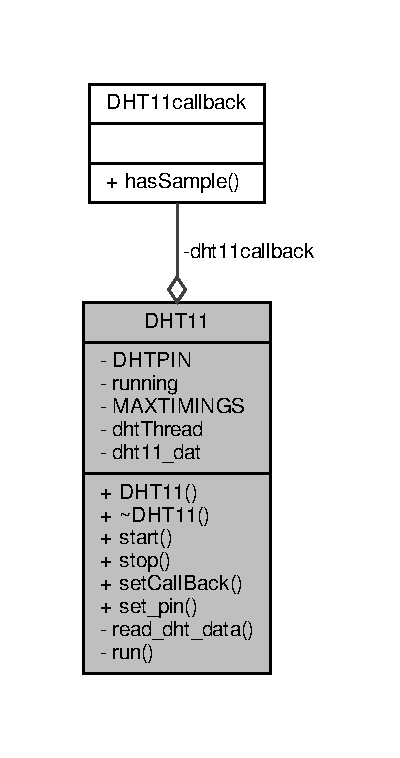
\includegraphics[width=192pt]{classDHT11__coll__graph}
\end{center}
\end{figure}
\subsection*{Public Member Functions}
\begin{DoxyCompactItemize}
\item 
\hyperlink{classDHT11_ad52a70ab511e087aaad53848d64ee976}{D\+H\+T11} (int pin)
\item 
\hyperlink{classDHT11_af210e94620802c4dd3a32f826b9cc389}{$\sim$\+D\+H\+T11} ()
\item 
void \hyperlink{classDHT11_a09a0c99de09f1849342d436624251f1d}{start} ()
\item 
void \hyperlink{classDHT11_a53188c041b8c49557d328f18ffbdacd7}{stop} ()
\item 
void \hyperlink{classDHT11_aeb671153e6b5db00efdf2ab654c45cb6}{set\+Call\+Back} (\hyperlink{classDHT11callback}{D\+H\+T11callback} $\ast$cb)
\item 
void \hyperlink{classDHT11_aa39533ef269048f791167e05598757fe}{set\+\_\+pin} (int pin)
\end{DoxyCompactItemize}
\subsection*{Private Member Functions}
\begin{DoxyCompactItemize}
\item 
bool \hyperlink{classDHT11_abf4c039a75c0458ee45621c12feec0c7}{read\+\_\+dht\+\_\+data} ()
\end{DoxyCompactItemize}
\subsection*{Static Private Member Functions}
\begin{DoxyCompactItemize}
\item 
static void \hyperlink{classDHT11_ae1a44c906a97ff4398d4d6721a1c8780}{run} (\hyperlink{classDHT11}{D\+H\+T11} $\ast$dht11)
\end{DoxyCompactItemize}
\subsection*{Private Attributes}
\begin{DoxyCompactItemize}
\item 
\hyperlink{classDHT11callback}{D\+H\+T11callback} $\ast$ \hyperlink{classDHT11_aebe3e30af75be9b419eb2fde69cfc00d}{dht11callback} = N\+U\+LL
\item 
int \hyperlink{classDHT11_a4d99108d62275d5ccf72df9d17b3211b}{D\+H\+T\+P\+IN}
\item 
int \hyperlink{classDHT11_a5e1eeeaac76105d3c7db78b63cab007d}{running} = 0
\item 
const int \hyperlink{classDHT11_aba8c5976478e858ec94a70d29deac72d}{M\+A\+X\+T\+I\+M\+I\+N\+GS} = 85
\item 
std\+::thread $\ast$ \hyperlink{classDHT11_a5e25d02345012c339d450951df5cebf7}{dht\+Thread} = N\+U\+LL
\item 
int \hyperlink{classDHT11_aa90815a46d88e84c34f091bf8f208315}{dht11\+\_\+dat} \mbox{[}5\mbox{]} = \{ 0, 0, 0, 0, 0 \}
\end{DoxyCompactItemize}


\subsection{Detailed Description}
This class reads data from D\+H\+T11/22 sensors in the background and calls a callback whenever data is available 

\subsection{Constructor \& Destructor Documentation}
\mbox{\Hypertarget{classDHT11_ad52a70ab511e087aaad53848d64ee976}\label{classDHT11_ad52a70ab511e087aaad53848d64ee976}} 
\index{D\+H\+T11@{D\+H\+T11}!D\+H\+T11@{D\+H\+T11}}
\index{D\+H\+T11@{D\+H\+T11}!D\+H\+T11@{D\+H\+T11}}
\subsubsection{\texorpdfstring{D\+H\+T11()}{DHT11()}}
{\footnotesize\ttfamily D\+H\+T11\+::\+D\+H\+T11 (\begin{DoxyParamCaption}\item[{int}]{pin }\end{DoxyParamCaption})}

clas constructor Here is the call graph for this function\+:
\nopagebreak
\begin{figure}[H]
\begin{center}
\leavevmode
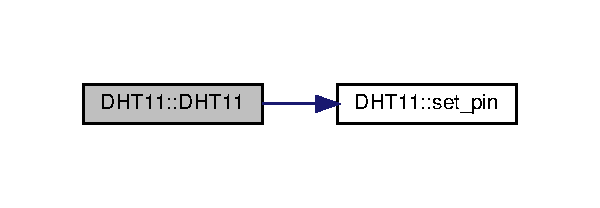
\includegraphics[width=288pt]{classDHT11_ad52a70ab511e087aaad53848d64ee976_cgraph}
\end{center}
\end{figure}
\mbox{\Hypertarget{classDHT11_af210e94620802c4dd3a32f826b9cc389}\label{classDHT11_af210e94620802c4dd3a32f826b9cc389}} 
\index{D\+H\+T11@{D\+H\+T11}!````~D\+H\+T11@{$\sim$\+D\+H\+T11}}
\index{````~D\+H\+T11@{$\sim$\+D\+H\+T11}!D\+H\+T11@{D\+H\+T11}}
\subsubsection{\texorpdfstring{$\sim$\+D\+H\+T11()}{~DHT11()}}
{\footnotesize\ttfamily D\+H\+T11\+::$\sim$\+D\+H\+T11 (\begin{DoxyParamCaption}{ }\end{DoxyParamCaption})\hspace{0.3cm}{\ttfamily [inline]}}



\subsection{Member Function Documentation}
\mbox{\Hypertarget{classDHT11_abf4c039a75c0458ee45621c12feec0c7}\label{classDHT11_abf4c039a75c0458ee45621c12feec0c7}} 
\index{D\+H\+T11@{D\+H\+T11}!read\+\_\+dht\+\_\+data@{read\+\_\+dht\+\_\+data}}
\index{read\+\_\+dht\+\_\+data@{read\+\_\+dht\+\_\+data}!D\+H\+T11@{D\+H\+T11}}
\subsubsection{\texorpdfstring{read\+\_\+dht\+\_\+data()}{read\_dht\_data()}}
{\footnotesize\ttfamily bool D\+H\+T11\+::read\+\_\+dht\+\_\+data (\begin{DoxyParamCaption}{ }\end{DoxyParamCaption})\hspace{0.3cm}{\ttfamily [private]}}

Here is the caller graph for this function\+:
\nopagebreak
\begin{figure}[H]
\begin{center}
\leavevmode
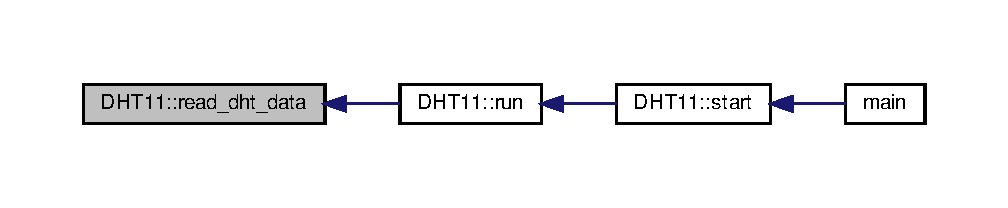
\includegraphics[width=350pt]{classDHT11_abf4c039a75c0458ee45621c12feec0c7_icgraph}
\end{center}
\end{figure}
\mbox{\Hypertarget{classDHT11_ae1a44c906a97ff4398d4d6721a1c8780}\label{classDHT11_ae1a44c906a97ff4398d4d6721a1c8780}} 
\index{D\+H\+T11@{D\+H\+T11}!run@{run}}
\index{run@{run}!D\+H\+T11@{D\+H\+T11}}
\subsubsection{\texorpdfstring{run()}{run()}}
{\footnotesize\ttfamily void D\+H\+T11\+::run (\begin{DoxyParamCaption}\item[{\hyperlink{classDHT11}{D\+H\+T11} $\ast$}]{dht11 }\end{DoxyParamCaption})\hspace{0.3cm}{\ttfamily [static]}, {\ttfamily [private]}}

Here is the call graph for this function\+:
\nopagebreak
\begin{figure}[H]
\begin{center}
\leavevmode
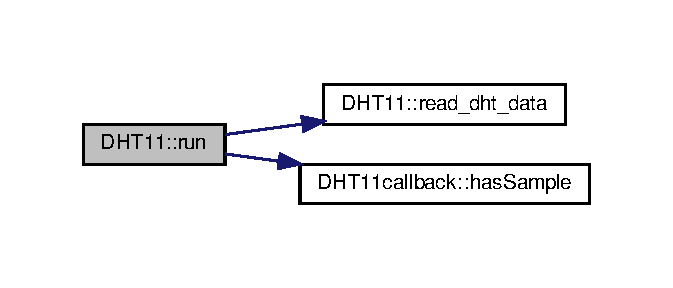
\includegraphics[width=323pt]{classDHT11_ae1a44c906a97ff4398d4d6721a1c8780_cgraph}
\end{center}
\end{figure}
Here is the caller graph for this function\+:
\nopagebreak
\begin{figure}[H]
\begin{center}
\leavevmode
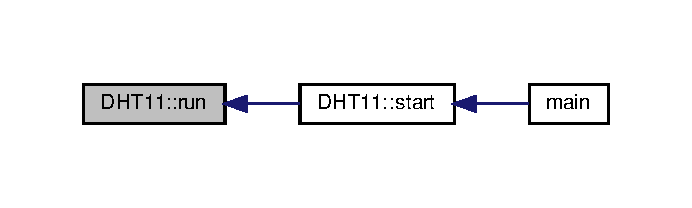
\includegraphics[width=332pt]{classDHT11_ae1a44c906a97ff4398d4d6721a1c8780_icgraph}
\end{center}
\end{figure}
\mbox{\Hypertarget{classDHT11_aa39533ef269048f791167e05598757fe}\label{classDHT11_aa39533ef269048f791167e05598757fe}} 
\index{D\+H\+T11@{D\+H\+T11}!set\+\_\+pin@{set\+\_\+pin}}
\index{set\+\_\+pin@{set\+\_\+pin}!D\+H\+T11@{D\+H\+T11}}
\subsubsection{\texorpdfstring{set\+\_\+pin()}{set\_pin()}}
{\footnotesize\ttfamily void D\+H\+T11\+::set\+\_\+pin (\begin{DoxyParamCaption}\item[{int}]{pin }\end{DoxyParamCaption})}

function that allows to set the G\+P\+IO pin Here is the caller graph for this function\+:
\nopagebreak
\begin{figure}[H]
\begin{center}
\leavevmode
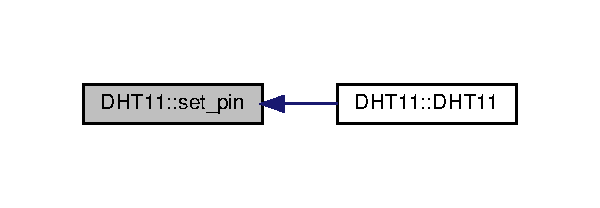
\includegraphics[width=288pt]{classDHT11_aa39533ef269048f791167e05598757fe_icgraph}
\end{center}
\end{figure}
\mbox{\Hypertarget{classDHT11_aeb671153e6b5db00efdf2ab654c45cb6}\label{classDHT11_aeb671153e6b5db00efdf2ab654c45cb6}} 
\index{D\+H\+T11@{D\+H\+T11}!set\+Call\+Back@{set\+Call\+Back}}
\index{set\+Call\+Back@{set\+Call\+Back}!D\+H\+T11@{D\+H\+T11}}
\subsubsection{\texorpdfstring{set\+Call\+Back()}{setCallBack()}}
{\footnotesize\ttfamily void D\+H\+T11\+::set\+Call\+Back (\begin{DoxyParamCaption}\item[{\hyperlink{classDHT11callback}{D\+H\+T11callback} $\ast$}]{cb }\end{DoxyParamCaption})}

function that allows to threads to set callbacks Here is the caller graph for this function\+:
\nopagebreak
\begin{figure}[H]
\begin{center}
\leavevmode
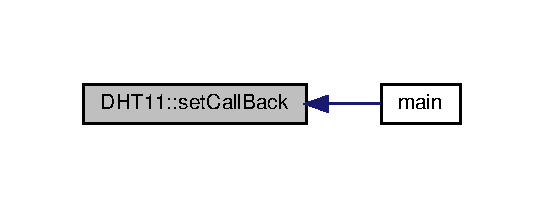
\includegraphics[width=261pt]{classDHT11_aeb671153e6b5db00efdf2ab654c45cb6_icgraph}
\end{center}
\end{figure}
\mbox{\Hypertarget{classDHT11_a09a0c99de09f1849342d436624251f1d}\label{classDHT11_a09a0c99de09f1849342d436624251f1d}} 
\index{D\+H\+T11@{D\+H\+T11}!start@{start}}
\index{start@{start}!D\+H\+T11@{D\+H\+T11}}
\subsubsection{\texorpdfstring{start()}{start()}}
{\footnotesize\ttfamily void D\+H\+T11\+::start (\begin{DoxyParamCaption}{ }\end{DoxyParamCaption})}

Starts the data acquisition in the background and the callback is called with new samples Here is the call graph for this function\+:
\nopagebreak
\begin{figure}[H]
\begin{center}
\leavevmode
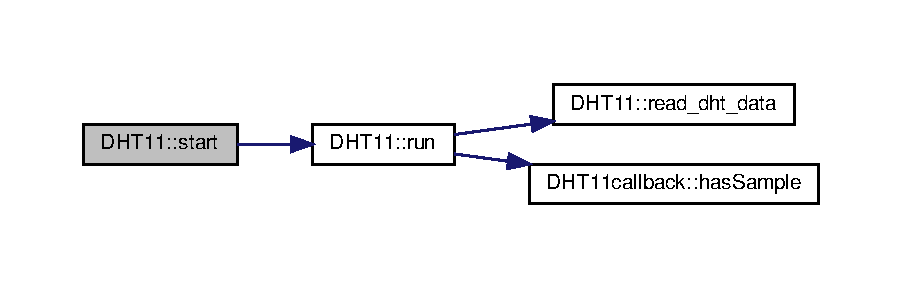
\includegraphics[width=350pt]{classDHT11_a09a0c99de09f1849342d436624251f1d_cgraph}
\end{center}
\end{figure}
Here is the caller graph for this function\+:
\nopagebreak
\begin{figure}[H]
\begin{center}
\leavevmode
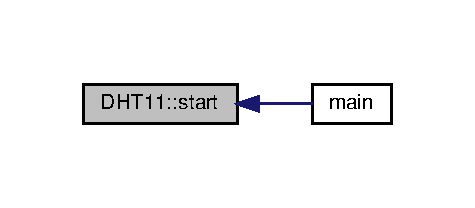
\includegraphics[width=228pt]{classDHT11_a09a0c99de09f1849342d436624251f1d_icgraph}
\end{center}
\end{figure}
\mbox{\Hypertarget{classDHT11_a53188c041b8c49557d328f18ffbdacd7}\label{classDHT11_a53188c041b8c49557d328f18ffbdacd7}} 
\index{D\+H\+T11@{D\+H\+T11}!stop@{stop}}
\index{stop@{stop}!D\+H\+T11@{D\+H\+T11}}
\subsubsection{\texorpdfstring{stop()}{stop()}}
{\footnotesize\ttfamily void D\+H\+T11\+::stop (\begin{DoxyParamCaption}{ }\end{DoxyParamCaption})}

Stops the data acquisition Here is the caller graph for this function\+:
\nopagebreak
\begin{figure}[H]
\begin{center}
\leavevmode
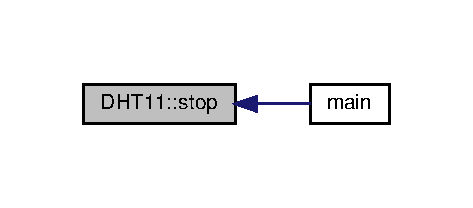
\includegraphics[width=227pt]{classDHT11_a53188c041b8c49557d328f18ffbdacd7_icgraph}
\end{center}
\end{figure}


\subsection{Field Documentation}
\mbox{\Hypertarget{classDHT11_aa90815a46d88e84c34f091bf8f208315}\label{classDHT11_aa90815a46d88e84c34f091bf8f208315}} 
\index{D\+H\+T11@{D\+H\+T11}!dht11\+\_\+dat@{dht11\+\_\+dat}}
\index{dht11\+\_\+dat@{dht11\+\_\+dat}!D\+H\+T11@{D\+H\+T11}}
\subsubsection{\texorpdfstring{dht11\+\_\+dat}{dht11\_dat}}
{\footnotesize\ttfamily int D\+H\+T11\+::dht11\+\_\+dat\mbox{[}5\mbox{]} = \{ 0, 0, 0, 0, 0 \}\hspace{0.3cm}{\ttfamily [private]}}

\mbox{\Hypertarget{classDHT11_aebe3e30af75be9b419eb2fde69cfc00d}\label{classDHT11_aebe3e30af75be9b419eb2fde69cfc00d}} 
\index{D\+H\+T11@{D\+H\+T11}!dht11callback@{dht11callback}}
\index{dht11callback@{dht11callback}!D\+H\+T11@{D\+H\+T11}}
\subsubsection{\texorpdfstring{dht11callback}{dht11callback}}
{\footnotesize\ttfamily \hyperlink{classDHT11callback}{D\+H\+T11callback}$\ast$ D\+H\+T11\+::dht11callback = N\+U\+LL\hspace{0.3cm}{\ttfamily [private]}}

\mbox{\Hypertarget{classDHT11_a4d99108d62275d5ccf72df9d17b3211b}\label{classDHT11_a4d99108d62275d5ccf72df9d17b3211b}} 
\index{D\+H\+T11@{D\+H\+T11}!D\+H\+T\+P\+IN@{D\+H\+T\+P\+IN}}
\index{D\+H\+T\+P\+IN@{D\+H\+T\+P\+IN}!D\+H\+T11@{D\+H\+T11}}
\subsubsection{\texorpdfstring{D\+H\+T\+P\+IN}{DHTPIN}}
{\footnotesize\ttfamily int D\+H\+T11\+::\+D\+H\+T\+P\+IN\hspace{0.3cm}{\ttfamily [private]}}

\mbox{\Hypertarget{classDHT11_a5e25d02345012c339d450951df5cebf7}\label{classDHT11_a5e25d02345012c339d450951df5cebf7}} 
\index{D\+H\+T11@{D\+H\+T11}!dht\+Thread@{dht\+Thread}}
\index{dht\+Thread@{dht\+Thread}!D\+H\+T11@{D\+H\+T11}}
\subsubsection{\texorpdfstring{dht\+Thread}{dhtThread}}
{\footnotesize\ttfamily std\+::thread$\ast$ D\+H\+T11\+::dht\+Thread = N\+U\+LL\hspace{0.3cm}{\ttfamily [private]}}

\mbox{\Hypertarget{classDHT11_aba8c5976478e858ec94a70d29deac72d}\label{classDHT11_aba8c5976478e858ec94a70d29deac72d}} 
\index{D\+H\+T11@{D\+H\+T11}!M\+A\+X\+T\+I\+M\+I\+N\+GS@{M\+A\+X\+T\+I\+M\+I\+N\+GS}}
\index{M\+A\+X\+T\+I\+M\+I\+N\+GS@{M\+A\+X\+T\+I\+M\+I\+N\+GS}!D\+H\+T11@{D\+H\+T11}}
\subsubsection{\texorpdfstring{M\+A\+X\+T\+I\+M\+I\+N\+GS}{MAXTIMINGS}}
{\footnotesize\ttfamily const int D\+H\+T11\+::\+M\+A\+X\+T\+I\+M\+I\+N\+GS = 85\hspace{0.3cm}{\ttfamily [private]}}

\mbox{\Hypertarget{classDHT11_a5e1eeeaac76105d3c7db78b63cab007d}\label{classDHT11_a5e1eeeaac76105d3c7db78b63cab007d}} 
\index{D\+H\+T11@{D\+H\+T11}!running@{running}}
\index{running@{running}!D\+H\+T11@{D\+H\+T11}}
\subsubsection{\texorpdfstring{running}{running}}
{\footnotesize\ttfamily int D\+H\+T11\+::running = 0\hspace{0.3cm}{\ttfamily [private]}}



The documentation for this class was generated from the following files\+:\begin{DoxyCompactItemize}
\item 
src/\hyperlink{DHT11_8h}{D\+H\+T11.\+h}\item 
src/\hyperlink{DHT11_8cpp}{D\+H\+T11.\+cpp}\end{DoxyCompactItemize}

\hypertarget{classDHT11callback}{}\section{D\+H\+T11callback Class Reference}
\label{classDHT11callback}\index{D\+H\+T11callback@{D\+H\+T11callback}}


{\ttfamily \#include $<$D\+H\+T11.\+h$>$}



Inheritance diagram for D\+H\+T11callback\+:
\nopagebreak
\begin{figure}[H]
\begin{center}
\leavevmode
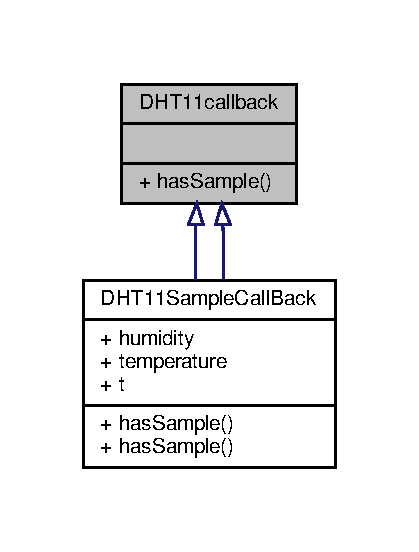
\includegraphics[width=201pt]{classDHT11callback__inherit__graph}
\end{center}
\end{figure}


Collaboration diagram for D\+H\+T11callback\+:
\nopagebreak
\begin{figure}[H]
\begin{center}
\leavevmode
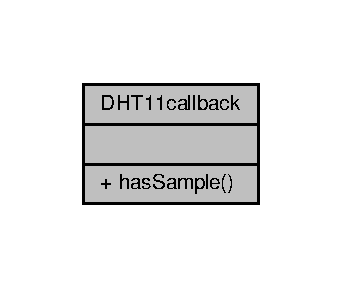
\includegraphics[width=164pt]{classDHT11callback__coll__graph}
\end{center}
\end{figure}
\subsection*{Public Member Functions}
\begin{DoxyCompactItemize}
\item 
virtual void \hyperlink{classDHT11callback_a57f4987fa9018acd572166a6c62b57d6}{has\+Sample} (int $\ast$data)=0
\end{DoxyCompactItemize}


\subsection{Detailed Description}
Callback for new samples which needs to be implemented by the main program. The function has\+Sample needs to be overloaded in the main program. 

\subsection{Member Function Documentation}
\mbox{\Hypertarget{classDHT11callback_a57f4987fa9018acd572166a6c62b57d6}\label{classDHT11callback_a57f4987fa9018acd572166a6c62b57d6}} 
\index{D\+H\+T11callback@{D\+H\+T11callback}!has\+Sample@{has\+Sample}}
\index{has\+Sample@{has\+Sample}!D\+H\+T11callback@{D\+H\+T11callback}}
\subsubsection{\texorpdfstring{has\+Sample()}{hasSample()}}
{\footnotesize\ttfamily virtual void D\+H\+T11callback\+::has\+Sample (\begin{DoxyParamCaption}\item[{int $\ast$}]{data }\end{DoxyParamCaption})\hspace{0.3cm}{\ttfamily [pure virtual]}}

Called after a sample has arrived. 

Implemented in \hyperlink{classDHT11SampleCallBack_a4545eba34196517369e67058f0e14e93}{D\+H\+T11\+Sample\+Call\+Back}, and \hyperlink{classDHT11SampleCallBack_a4545eba34196517369e67058f0e14e93}{D\+H\+T11\+Sample\+Call\+Back}.

Here is the caller graph for this function\+:
\nopagebreak
\begin{figure}[H]
\begin{center}
\leavevmode
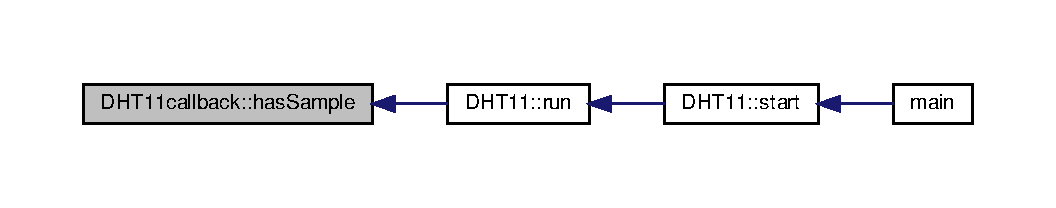
\includegraphics[width=350pt]{classDHT11callback_a57f4987fa9018acd572166a6c62b57d6_icgraph}
\end{center}
\end{figure}


The documentation for this class was generated from the following file\+:\begin{DoxyCompactItemize}
\item 
src/\hyperlink{DHT11_8h}{D\+H\+T11.\+h}\end{DoxyCompactItemize}

\hypertarget{classDHT11SampleCallBack}{}\section{D\+H\+T11\+Sample\+Call\+Back Class Reference}
\label{classDHT11SampleCallBack}\index{D\+H\+T11\+Sample\+Call\+Back@{D\+H\+T11\+Sample\+Call\+Back}}


Inheritance diagram for D\+H\+T11\+Sample\+Call\+Back\+:
\nopagebreak
\begin{figure}[H]
\begin{center}
\leavevmode
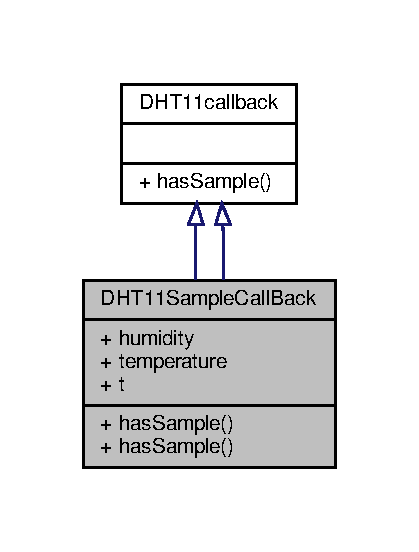
\includegraphics[width=201pt]{classDHT11SampleCallBack__inherit__graph}
\end{center}
\end{figure}


Collaboration diagram for D\+H\+T11\+Sample\+Call\+Back\+:
\nopagebreak
\begin{figure}[H]
\begin{center}
\leavevmode
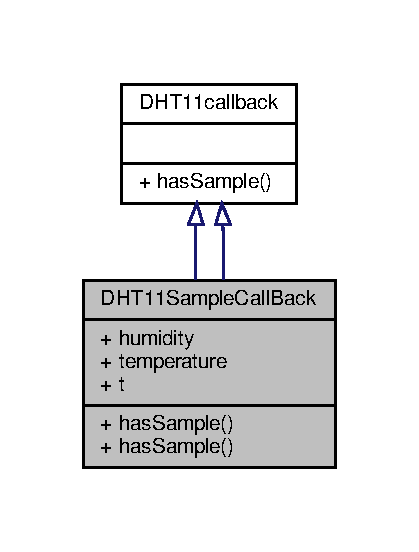
\includegraphics[width=201pt]{classDHT11SampleCallBack__coll__graph}
\end{center}
\end{figure}
\subsection*{Public Member Functions}
\begin{DoxyCompactItemize}
\item 
virtual void \hyperlink{classDHT11SampleCallBack_a4545eba34196517369e67058f0e14e93}{has\+Sample} (int $\ast$data)
\item 
virtual void \hyperlink{classDHT11SampleCallBack_a4545eba34196517369e67058f0e14e93}{has\+Sample} (int $\ast$data)
\end{DoxyCompactItemize}
\subsection*{Data Fields}
\begin{DoxyCompactItemize}
\item 
float \hyperlink{classDHT11SampleCallBack_aea1bc3b1d58de0365f32bf5098cd5734}{humidity}
\item 
float \hyperlink{classDHT11SampleCallBack_a897d17761377313be39c9e974a7df3f4}{temperature}
\item 
long \hyperlink{classDHT11SampleCallBack_a2a60b640929f5f6de7be95455f6cc365}{t}
\end{DoxyCompactItemize}


\subsection{Member Function Documentation}
\mbox{\Hypertarget{classDHT11SampleCallBack_a4545eba34196517369e67058f0e14e93}\label{classDHT11SampleCallBack_a4545eba34196517369e67058f0e14e93}} 
\index{D\+H\+T11\+Sample\+Call\+Back@{D\+H\+T11\+Sample\+Call\+Back}!has\+Sample@{has\+Sample}}
\index{has\+Sample@{has\+Sample}!D\+H\+T11\+Sample\+Call\+Back@{D\+H\+T11\+Sample\+Call\+Back}}
\subsubsection{\texorpdfstring{has\+Sample()}{hasSample()}\hspace{0.1cm}{\footnotesize\ttfamily [1/2]}}
{\footnotesize\ttfamily virtual void D\+H\+T11\+Sample\+Call\+Back\+::has\+Sample (\begin{DoxyParamCaption}\item[{int $\ast$}]{data }\end{DoxyParamCaption})\hspace{0.3cm}{\ttfamily [inline]}, {\ttfamily [virtual]}}

Called after a sample has arrived. 

Implements \hyperlink{classDHT11callback_a57f4987fa9018acd572166a6c62b57d6}{D\+H\+T11callback}.

\mbox{\Hypertarget{classDHT11SampleCallBack_a4545eba34196517369e67058f0e14e93}\label{classDHT11SampleCallBack_a4545eba34196517369e67058f0e14e93}} 
\index{D\+H\+T11\+Sample\+Call\+Back@{D\+H\+T11\+Sample\+Call\+Back}!has\+Sample@{has\+Sample}}
\index{has\+Sample@{has\+Sample}!D\+H\+T11\+Sample\+Call\+Back@{D\+H\+T11\+Sample\+Call\+Back}}
\subsubsection{\texorpdfstring{has\+Sample()}{hasSample()}\hspace{0.1cm}{\footnotesize\ttfamily [2/2]}}
{\footnotesize\ttfamily virtual void D\+H\+T11\+Sample\+Call\+Back\+::has\+Sample (\begin{DoxyParamCaption}\item[{int $\ast$}]{data }\end{DoxyParamCaption})\hspace{0.3cm}{\ttfamily [inline]}, {\ttfamily [virtual]}}

Called after a sample has arrived. 

Implements \hyperlink{classDHT11callback_a57f4987fa9018acd572166a6c62b57d6}{D\+H\+T11callback}.



\subsection{Field Documentation}
\mbox{\Hypertarget{classDHT11SampleCallBack_aea1bc3b1d58de0365f32bf5098cd5734}\label{classDHT11SampleCallBack_aea1bc3b1d58de0365f32bf5098cd5734}} 
\index{D\+H\+T11\+Sample\+Call\+Back@{D\+H\+T11\+Sample\+Call\+Back}!humidity@{humidity}}
\index{humidity@{humidity}!D\+H\+T11\+Sample\+Call\+Back@{D\+H\+T11\+Sample\+Call\+Back}}
\subsubsection{\texorpdfstring{humidity}{humidity}}
{\footnotesize\ttfamily float D\+H\+T11\+Sample\+Call\+Back\+::humidity}

\mbox{\Hypertarget{classDHT11SampleCallBack_a2a60b640929f5f6de7be95455f6cc365}\label{classDHT11SampleCallBack_a2a60b640929f5f6de7be95455f6cc365}} 
\index{D\+H\+T11\+Sample\+Call\+Back@{D\+H\+T11\+Sample\+Call\+Back}!t@{t}}
\index{t@{t}!D\+H\+T11\+Sample\+Call\+Back@{D\+H\+T11\+Sample\+Call\+Back}}
\subsubsection{\texorpdfstring{t}{t}}
{\footnotesize\ttfamily long D\+H\+T11\+Sample\+Call\+Back\+::t}

\mbox{\Hypertarget{classDHT11SampleCallBack_a897d17761377313be39c9e974a7df3f4}\label{classDHT11SampleCallBack_a897d17761377313be39c9e974a7df3f4}} 
\index{D\+H\+T11\+Sample\+Call\+Back@{D\+H\+T11\+Sample\+Call\+Back}!temperature@{temperature}}
\index{temperature@{temperature}!D\+H\+T11\+Sample\+Call\+Back@{D\+H\+T11\+Sample\+Call\+Back}}
\subsubsection{\texorpdfstring{temperature}{temperature}}
{\footnotesize\ttfamily float D\+H\+T11\+Sample\+Call\+Back\+::temperature}



The documentation for this class was generated from the following files\+:\begin{DoxyCompactItemize}
\item 
src/\hyperlink{demo_8cpp}{demo.\+cpp}\item 
src/\hyperlink{dht11__callback_8cpp}{dht11\+\_\+callback.\+cpp}\end{DoxyCompactItemize}

\hypertarget{classJSONCGIHandler_1_1GETCallback}{}\section{J\+S\+O\+N\+C\+G\+I\+Handler\+:\+:G\+E\+T\+Callback Class Reference}
\label{classJSONCGIHandler_1_1GETCallback}\index{J\+S\+O\+N\+C\+G\+I\+Handler\+::\+G\+E\+T\+Callback@{J\+S\+O\+N\+C\+G\+I\+Handler\+::\+G\+E\+T\+Callback}}


{\ttfamily \#include $<$json\+\_\+fastcgi\+\_\+web\+\_\+api.\+h$>$}



Inheritance diagram for J\+S\+O\+N\+C\+G\+I\+Handler\+:\+:G\+E\+T\+Callback\+:
\nopagebreak
\begin{figure}[H]
\begin{center}
\leavevmode
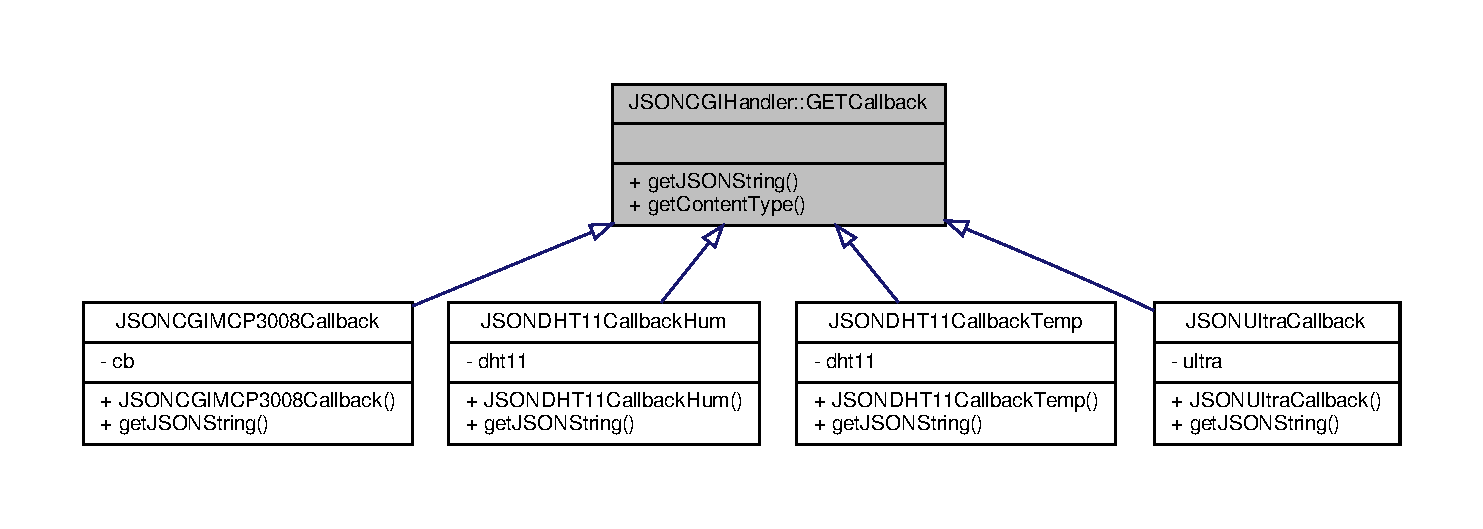
\includegraphics[width=350pt]{classJSONCGIHandler_1_1GETCallback__inherit__graph}
\end{center}
\end{figure}


Collaboration diagram for J\+S\+O\+N\+C\+G\+I\+Handler\+:\+:G\+E\+T\+Callback\+:
\nopagebreak
\begin{figure}[H]
\begin{center}
\leavevmode
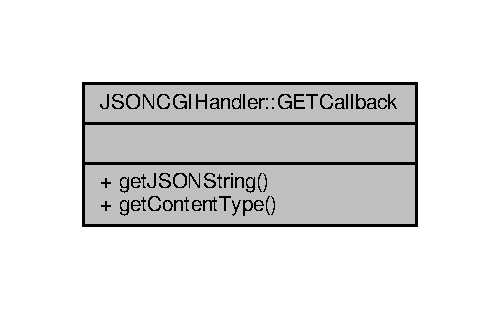
\includegraphics[width=240pt]{classJSONCGIHandler_1_1GETCallback__coll__graph}
\end{center}
\end{figure}
\subsection*{Public Member Functions}
\begin{DoxyCompactItemize}
\item 
virtual std\+::string \hyperlink{classJSONCGIHandler_1_1GETCallback_a2367bf5a5912e9e5599ee464e0846255}{get\+J\+S\+O\+N\+String} ()=0
\item 
virtual std\+::string \hyperlink{classJSONCGIHandler_1_1GETCallback_a4e1fee495ddeb4e24eaa5b8e767ea838}{get\+Content\+Type} ()
\end{DoxyCompactItemize}


\subsection{Detailed Description}
G\+ET callback handler which needs to be implemented by the main program. This needs to provide the J\+S\+ON payload as a string either by using the simple \hyperlink{classJSONCGIHandler_1_1JSONGenerator}{J\+S\+O\+N\+Generator} or by an external library. 

\subsection{Member Function Documentation}
\mbox{\Hypertarget{classJSONCGIHandler_1_1GETCallback_a4e1fee495ddeb4e24eaa5b8e767ea838}\label{classJSONCGIHandler_1_1GETCallback_a4e1fee495ddeb4e24eaa5b8e767ea838}} 
\index{J\+S\+O\+N\+C\+G\+I\+Handler\+::\+G\+E\+T\+Callback@{J\+S\+O\+N\+C\+G\+I\+Handler\+::\+G\+E\+T\+Callback}!get\+Content\+Type@{get\+Content\+Type}}
\index{get\+Content\+Type@{get\+Content\+Type}!J\+S\+O\+N\+C\+G\+I\+Handler\+::\+G\+E\+T\+Callback@{J\+S\+O\+N\+C\+G\+I\+Handler\+::\+G\+E\+T\+Callback}}
\subsubsection{\texorpdfstring{get\+Content\+Type()}{getContentType()}}
{\footnotesize\ttfamily virtual std\+::string J\+S\+O\+N\+C\+G\+I\+Handler\+::\+G\+E\+T\+Callback\+::get\+Content\+Type (\begin{DoxyParamCaption}{ }\end{DoxyParamCaption})\hspace{0.3cm}{\ttfamily [inline]}, {\ttfamily [virtual]}}

The content type of the payload. That\textquotesingle{}s by default \char`\"{}application/json\char`\"{} but can be overloaded if needed. \begin{DoxyReturn}{Returns}
M\+I\+ME type 
\end{DoxyReturn}
Here is the caller graph for this function\+:
\nopagebreak
\begin{figure}[H]
\begin{center}
\leavevmode
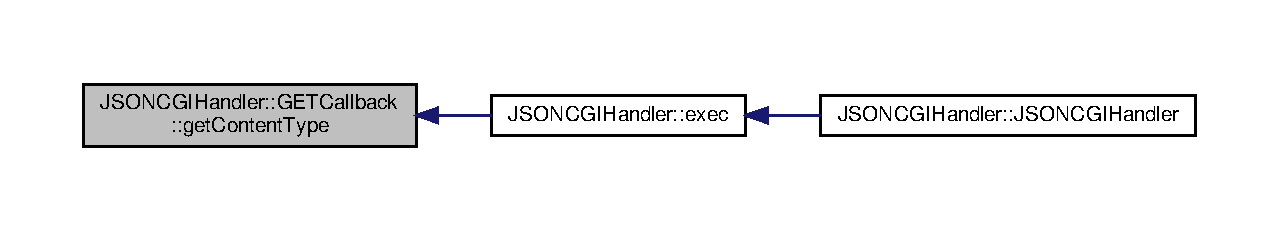
\includegraphics[width=350pt]{classJSONCGIHandler_1_1GETCallback_a4e1fee495ddeb4e24eaa5b8e767ea838_icgraph}
\end{center}
\end{figure}
\mbox{\Hypertarget{classJSONCGIHandler_1_1GETCallback_a2367bf5a5912e9e5599ee464e0846255}\label{classJSONCGIHandler_1_1GETCallback_a2367bf5a5912e9e5599ee464e0846255}} 
\index{J\+S\+O\+N\+C\+G\+I\+Handler\+::\+G\+E\+T\+Callback@{J\+S\+O\+N\+C\+G\+I\+Handler\+::\+G\+E\+T\+Callback}!get\+J\+S\+O\+N\+String@{get\+J\+S\+O\+N\+String}}
\index{get\+J\+S\+O\+N\+String@{get\+J\+S\+O\+N\+String}!J\+S\+O\+N\+C\+G\+I\+Handler\+::\+G\+E\+T\+Callback@{J\+S\+O\+N\+C\+G\+I\+Handler\+::\+G\+E\+T\+Callback}}
\subsubsection{\texorpdfstring{get\+J\+S\+O\+N\+String()}{getJSONString()}}
{\footnotesize\ttfamily virtual std\+::string J\+S\+O\+N\+C\+G\+I\+Handler\+::\+G\+E\+T\+Callback\+::get\+J\+S\+O\+N\+String (\begin{DoxyParamCaption}{ }\end{DoxyParamCaption})\hspace{0.3cm}{\ttfamily [pure virtual]}}

Needs to return the payload data sent to the web browser. Use the \hyperlink{classJSONCGIHandler_1_1JSONGenerator}{J\+S\+O\+N\+Generator} to create the J\+S\+ON or use an external json generator. \begin{DoxyReturn}{Returns}
J\+S\+ON data 
\end{DoxyReturn}


Implemented in \hyperlink{classJSONUltraCallback_abb097f82255b74c56370b90bc06d81da}{J\+S\+O\+N\+Ultra\+Callback}, \hyperlink{classJSONDHT11CallbackHum_acc4cc41772967e063e1364d7c92ab985}{J\+S\+O\+N\+D\+H\+T11\+Callback\+Hum}, \hyperlink{classJSONDHT11CallbackTemp_afe3fed3115bf659bdeb92463c7965dac}{J\+S\+O\+N\+D\+H\+T11\+Callback\+Temp}, and \hyperlink{classJSONCGIMCP3008Callback_aac6e6543d0b4da62f72781f3fe47ebed}{J\+S\+O\+N\+C\+G\+I\+M\+C\+P3008\+Callback}.

Here is the caller graph for this function\+:
\nopagebreak
\begin{figure}[H]
\begin{center}
\leavevmode
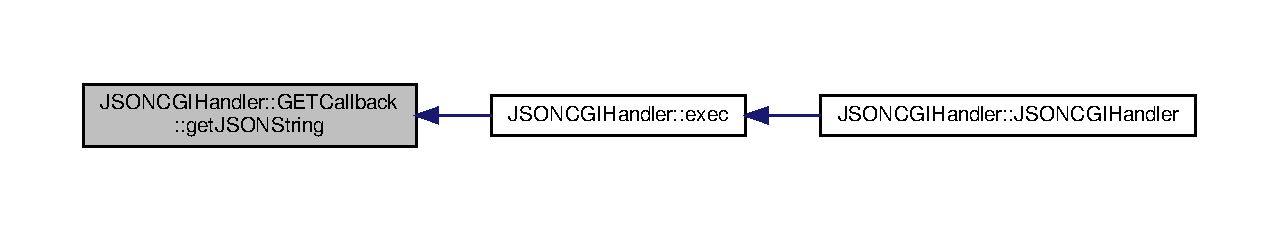
\includegraphics[width=350pt]{classJSONCGIHandler_1_1GETCallback_a2367bf5a5912e9e5599ee464e0846255_icgraph}
\end{center}
\end{figure}


The documentation for this class was generated from the following file\+:\begin{DoxyCompactItemize}
\item 
src/\hyperlink{json__fastcgi__web__api_8h}{json\+\_\+fastcgi\+\_\+web\+\_\+api.\+h}\end{DoxyCompactItemize}

\hypertarget{classJSONCGIHandler}{}\section{J\+S\+O\+N\+C\+G\+I\+Handler Class Reference}
\label{classJSONCGIHandler}\index{J\+S\+O\+N\+C\+G\+I\+Handler@{J\+S\+O\+N\+C\+G\+I\+Handler}}


{\ttfamily \#include $<$json\+\_\+fastcgi\+\_\+web\+\_\+api.\+h$>$}



Collaboration diagram for J\+S\+O\+N\+C\+G\+I\+Handler\+:
\nopagebreak
\begin{figure}[H]
\begin{center}
\leavevmode
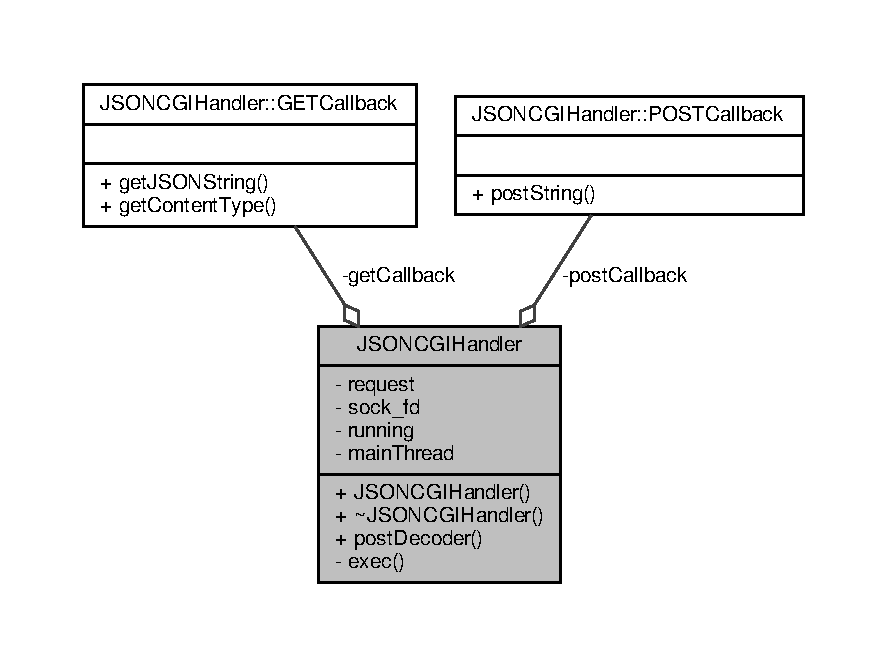
\includegraphics[width=350pt]{classJSONCGIHandler__coll__graph}
\end{center}
\end{figure}
\subsection*{Data Structures}
\begin{DoxyCompactItemize}
\item 
class \hyperlink{classJSONCGIHandler_1_1GETCallback}{G\+E\+T\+Callback}
\item 
class \hyperlink{classJSONCGIHandler_1_1JSONGenerator}{J\+S\+O\+N\+Generator}
\item 
class \hyperlink{classJSONCGIHandler_1_1POSTCallback}{P\+O\+S\+T\+Callback}
\end{DoxyCompactItemize}
\subsection*{Public Member Functions}
\begin{DoxyCompactItemize}
\item 
\hyperlink{classJSONCGIHandler_a9bf5a96d13949d363225561ba6ac3b56}{J\+S\+O\+N\+C\+G\+I\+Handler} (\hyperlink{classJSONCGIHandler_1_1GETCallback}{G\+E\+T\+Callback} $\ast$arg\+Get\+Callback, \hyperlink{classJSONCGIHandler_1_1POSTCallback}{P\+O\+S\+T\+Callback} $\ast$arg\+Post\+Callback=nullptr, const char socketpath\mbox{[}$\,$\mbox{]}=\char`\"{}/tmp/fastcgisocket\char`\"{})
\item 
\hyperlink{classJSONCGIHandler_a4817e428a962bdea68123f2d32671f30}{$\sim$\+J\+S\+O\+N\+C\+G\+I\+Handler} ()
\end{DoxyCompactItemize}
\subsection*{Static Public Member Functions}
\begin{DoxyCompactItemize}
\item 
static std\+::map$<$ std\+::string, std\+::string $>$ \hyperlink{classJSONCGIHandler_a0f208af3dd050ed182967fe9cca42d78}{post\+Decoder} (std\+::string s)
\end{DoxyCompactItemize}
\subsection*{Static Private Member Functions}
\begin{DoxyCompactItemize}
\item 
static void \hyperlink{classJSONCGIHandler_a42518cd5ad781476d299b50e4c4c0000}{exec} (\hyperlink{classJSONCGIHandler}{J\+S\+O\+N\+C\+G\+I\+Handler} $\ast$fast\+C\+G\+I\+Handler)
\end{DoxyCompactItemize}
\subsection*{Private Attributes}
\begin{DoxyCompactItemize}
\item 
F\+C\+G\+X\+\_\+\+Request \hyperlink{classJSONCGIHandler_a69dba19ef64e913fc7e969854be997c9}{request}
\item 
int \hyperlink{classJSONCGIHandler_a6f696ff6856f32b3ba75a130fcbb8987}{sock\+\_\+fd} = 0
\item 
int \hyperlink{classJSONCGIHandler_aefa19cd01b387693ef99c5aa0c5fc093}{running} = 1
\item 
std\+::thread $\ast$ \hyperlink{classJSONCGIHandler_aca513f708ae4dc76ba70196ff25da695}{main\+Thread} = nullptr
\item 
\hyperlink{classJSONCGIHandler_1_1GETCallback}{G\+E\+T\+Callback} $\ast$ \hyperlink{classJSONCGIHandler_a7c8b4a44e15ac57fe93b382e86899fa7}{get\+Callback} = nullptr
\item 
\hyperlink{classJSONCGIHandler_1_1POSTCallback}{P\+O\+S\+T\+Callback} $\ast$ \hyperlink{classJSONCGIHandler_a09ee0f555db808d07c9ee9a575780553}{post\+Callback} = nullptr
\end{DoxyCompactItemize}


\subsection{Detailed Description}
C++ wrapper around fast\+C\+GI which sends and receives J\+S\+ON in a j\+Query friendly format.

Copyright (C) 2021 Bernd Porr \href{mailto:mail@berndporr.me.uk}{\tt mail@berndporr.\+me.\+uk} Apache License 2.\+0 

\subsection{Constructor \& Destructor Documentation}
\mbox{\Hypertarget{classJSONCGIHandler_a9bf5a96d13949d363225561ba6ac3b56}\label{classJSONCGIHandler_a9bf5a96d13949d363225561ba6ac3b56}} 
\index{J\+S\+O\+N\+C\+G\+I\+Handler@{J\+S\+O\+N\+C\+G\+I\+Handler}!J\+S\+O\+N\+C\+G\+I\+Handler@{J\+S\+O\+N\+C\+G\+I\+Handler}}
\index{J\+S\+O\+N\+C\+G\+I\+Handler@{J\+S\+O\+N\+C\+G\+I\+Handler}!J\+S\+O\+N\+C\+G\+I\+Handler@{J\+S\+O\+N\+C\+G\+I\+Handler}}
\subsubsection{\texorpdfstring{J\+S\+O\+N\+C\+G\+I\+Handler()}{JSONCGIHandler()}}
{\footnotesize\ttfamily J\+S\+O\+N\+C\+G\+I\+Handler\+::\+J\+S\+O\+N\+C\+G\+I\+Handler (\begin{DoxyParamCaption}\item[{\hyperlink{classJSONCGIHandler_1_1GETCallback}{G\+E\+T\+Callback} $\ast$}]{arg\+Get\+Callback,  }\item[{\hyperlink{classJSONCGIHandler_1_1POSTCallback}{P\+O\+S\+T\+Callback} $\ast$}]{arg\+Post\+Callback = {\ttfamily nullptr},  }\item[{const char}]{socketpath\mbox{[}$\,$\mbox{]} = {\ttfamily \char`\"{}/tmp/fastcgisocket\char`\"{}} }\end{DoxyParamCaption})\hspace{0.3cm}{\ttfamily [inline]}}

Constructor which opens the connection and starts the main thread. Provide an instance of the callback handler which returns the payload data. arg\+Post\+Callback is the callback which returns received json packets as a map. The optional socketpath variable can be set to another path for the socket which talks to the webserver. 
\begin{DoxyParams}{Parameters}
{\em arg\+Get\+Callback} & Callback handler for sending J\+S\+ON \\
\hline
{\em arg\+Post\+Callback} & Callback handler for receiving J\+S\+ON \\
\hline
{\em socketpath} & Path of the socket which communicates to the webserver \\
\hline
\end{DoxyParams}
Here is the call graph for this function\+:
\nopagebreak
\begin{figure}[H]
\begin{center}
\leavevmode
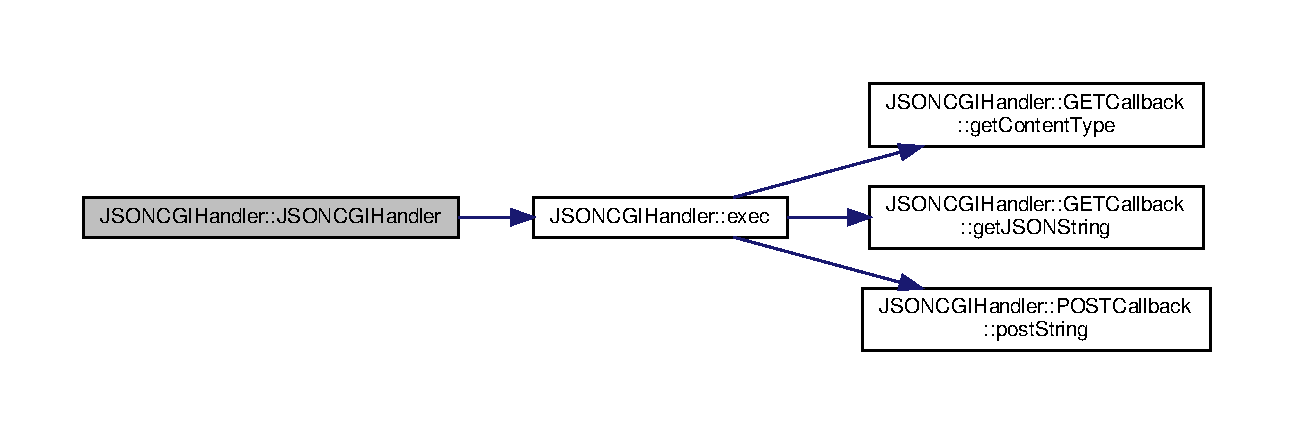
\includegraphics[width=350pt]{classJSONCGIHandler_a9bf5a96d13949d363225561ba6ac3b56_cgraph}
\end{center}
\end{figure}
\mbox{\Hypertarget{classJSONCGIHandler_a4817e428a962bdea68123f2d32671f30}\label{classJSONCGIHandler_a4817e428a962bdea68123f2d32671f30}} 
\index{J\+S\+O\+N\+C\+G\+I\+Handler@{J\+S\+O\+N\+C\+G\+I\+Handler}!````~J\+S\+O\+N\+C\+G\+I\+Handler@{$\sim$\+J\+S\+O\+N\+C\+G\+I\+Handler}}
\index{````~J\+S\+O\+N\+C\+G\+I\+Handler@{$\sim$\+J\+S\+O\+N\+C\+G\+I\+Handler}!J\+S\+O\+N\+C\+G\+I\+Handler@{J\+S\+O\+N\+C\+G\+I\+Handler}}
\subsubsection{\texorpdfstring{$\sim$\+J\+S\+O\+N\+C\+G\+I\+Handler()}{~JSONCGIHandler()}}
{\footnotesize\ttfamily J\+S\+O\+N\+C\+G\+I\+Handler\+::$\sim$\+J\+S\+O\+N\+C\+G\+I\+Handler (\begin{DoxyParamCaption}{ }\end{DoxyParamCaption})\hspace{0.3cm}{\ttfamily [inline]}}

Destructor which shuts down the connection to the webserver and it also terminates the thread which is waiting for requests. 

\subsection{Member Function Documentation}
\mbox{\Hypertarget{classJSONCGIHandler_a42518cd5ad781476d299b50e4c4c0000}\label{classJSONCGIHandler_a42518cd5ad781476d299b50e4c4c0000}} 
\index{J\+S\+O\+N\+C\+G\+I\+Handler@{J\+S\+O\+N\+C\+G\+I\+Handler}!exec@{exec}}
\index{exec@{exec}!J\+S\+O\+N\+C\+G\+I\+Handler@{J\+S\+O\+N\+C\+G\+I\+Handler}}
\subsubsection{\texorpdfstring{exec()}{exec()}}
{\footnotesize\ttfamily static void J\+S\+O\+N\+C\+G\+I\+Handler\+::exec (\begin{DoxyParamCaption}\item[{\hyperlink{classJSONCGIHandler}{J\+S\+O\+N\+C\+G\+I\+Handler} $\ast$}]{fast\+C\+G\+I\+Handler }\end{DoxyParamCaption})\hspace{0.3cm}{\ttfamily [inline]}, {\ttfamily [static]}, {\ttfamily [private]}}

Here is the call graph for this function\+:
\nopagebreak
\begin{figure}[H]
\begin{center}
\leavevmode
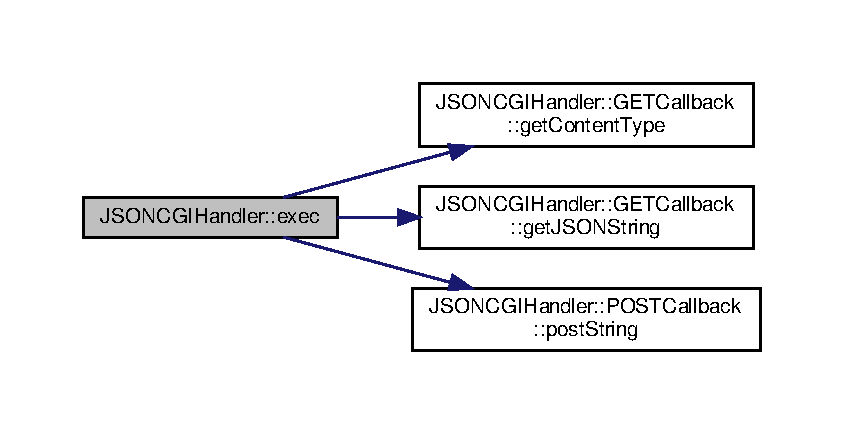
\includegraphics[width=350pt]{classJSONCGIHandler_a42518cd5ad781476d299b50e4c4c0000_cgraph}
\end{center}
\end{figure}
Here is the caller graph for this function\+:
\nopagebreak
\begin{figure}[H]
\begin{center}
\leavevmode
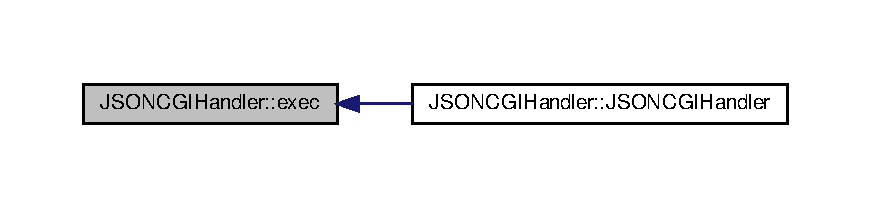
\includegraphics[width=350pt]{classJSONCGIHandler_a42518cd5ad781476d299b50e4c4c0000_icgraph}
\end{center}
\end{figure}
\mbox{\Hypertarget{classJSONCGIHandler_a0f208af3dd050ed182967fe9cca42d78}\label{classJSONCGIHandler_a0f208af3dd050ed182967fe9cca42d78}} 
\index{J\+S\+O\+N\+C\+G\+I\+Handler@{J\+S\+O\+N\+C\+G\+I\+Handler}!post\+Decoder@{post\+Decoder}}
\index{post\+Decoder@{post\+Decoder}!J\+S\+O\+N\+C\+G\+I\+Handler@{J\+S\+O\+N\+C\+G\+I\+Handler}}
\subsubsection{\texorpdfstring{post\+Decoder()}{postDecoder()}}
{\footnotesize\ttfamily static std\+::map$<$std\+::string,std\+::string$>$ J\+S\+O\+N\+C\+G\+I\+Handler\+::post\+Decoder (\begin{DoxyParamCaption}\item[{std\+::string}]{s }\end{DoxyParamCaption})\hspace{0.3cm}{\ttfamily [inline]}, {\ttfamily [static]}}

Parses a P\+O\+ST string and returns a std\+::map with key/value pairs. It also converts back any xx style encoding back to chars using libcurl. Note this is a simple parser and it won\textquotesingle{}t deal with nested J\+S\+ON structures. 
\begin{DoxyParams}{Parameters}
{\em s} & The P\+O\+ST string to be decoded. \\
\hline
\end{DoxyParams}
\begin{DoxyReturn}{Returns}
A std\+::map which conains the key/value pairs. 
\end{DoxyReturn}


\subsection{Field Documentation}
\mbox{\Hypertarget{classJSONCGIHandler_a7c8b4a44e15ac57fe93b382e86899fa7}\label{classJSONCGIHandler_a7c8b4a44e15ac57fe93b382e86899fa7}} 
\index{J\+S\+O\+N\+C\+G\+I\+Handler@{J\+S\+O\+N\+C\+G\+I\+Handler}!get\+Callback@{get\+Callback}}
\index{get\+Callback@{get\+Callback}!J\+S\+O\+N\+C\+G\+I\+Handler@{J\+S\+O\+N\+C\+G\+I\+Handler}}
\subsubsection{\texorpdfstring{get\+Callback}{getCallback}}
{\footnotesize\ttfamily \hyperlink{classJSONCGIHandler_1_1GETCallback}{G\+E\+T\+Callback}$\ast$ J\+S\+O\+N\+C\+G\+I\+Handler\+::get\+Callback = nullptr\hspace{0.3cm}{\ttfamily [private]}}

\mbox{\Hypertarget{classJSONCGIHandler_aca513f708ae4dc76ba70196ff25da695}\label{classJSONCGIHandler_aca513f708ae4dc76ba70196ff25da695}} 
\index{J\+S\+O\+N\+C\+G\+I\+Handler@{J\+S\+O\+N\+C\+G\+I\+Handler}!main\+Thread@{main\+Thread}}
\index{main\+Thread@{main\+Thread}!J\+S\+O\+N\+C\+G\+I\+Handler@{J\+S\+O\+N\+C\+G\+I\+Handler}}
\subsubsection{\texorpdfstring{main\+Thread}{mainThread}}
{\footnotesize\ttfamily std\+::thread$\ast$ J\+S\+O\+N\+C\+G\+I\+Handler\+::main\+Thread = nullptr\hspace{0.3cm}{\ttfamily [private]}}

\mbox{\Hypertarget{classJSONCGIHandler_a09ee0f555db808d07c9ee9a575780553}\label{classJSONCGIHandler_a09ee0f555db808d07c9ee9a575780553}} 
\index{J\+S\+O\+N\+C\+G\+I\+Handler@{J\+S\+O\+N\+C\+G\+I\+Handler}!post\+Callback@{post\+Callback}}
\index{post\+Callback@{post\+Callback}!J\+S\+O\+N\+C\+G\+I\+Handler@{J\+S\+O\+N\+C\+G\+I\+Handler}}
\subsubsection{\texorpdfstring{post\+Callback}{postCallback}}
{\footnotesize\ttfamily \hyperlink{classJSONCGIHandler_1_1POSTCallback}{P\+O\+S\+T\+Callback}$\ast$ J\+S\+O\+N\+C\+G\+I\+Handler\+::post\+Callback = nullptr\hspace{0.3cm}{\ttfamily [private]}}

\mbox{\Hypertarget{classJSONCGIHandler_a69dba19ef64e913fc7e969854be997c9}\label{classJSONCGIHandler_a69dba19ef64e913fc7e969854be997c9}} 
\index{J\+S\+O\+N\+C\+G\+I\+Handler@{J\+S\+O\+N\+C\+G\+I\+Handler}!request@{request}}
\index{request@{request}!J\+S\+O\+N\+C\+G\+I\+Handler@{J\+S\+O\+N\+C\+G\+I\+Handler}}
\subsubsection{\texorpdfstring{request}{request}}
{\footnotesize\ttfamily F\+C\+G\+X\+\_\+\+Request J\+S\+O\+N\+C\+G\+I\+Handler\+::request\hspace{0.3cm}{\ttfamily [private]}}

\mbox{\Hypertarget{classJSONCGIHandler_aefa19cd01b387693ef99c5aa0c5fc093}\label{classJSONCGIHandler_aefa19cd01b387693ef99c5aa0c5fc093}} 
\index{J\+S\+O\+N\+C\+G\+I\+Handler@{J\+S\+O\+N\+C\+G\+I\+Handler}!running@{running}}
\index{running@{running}!J\+S\+O\+N\+C\+G\+I\+Handler@{J\+S\+O\+N\+C\+G\+I\+Handler}}
\subsubsection{\texorpdfstring{running}{running}}
{\footnotesize\ttfamily int J\+S\+O\+N\+C\+G\+I\+Handler\+::running = 1\hspace{0.3cm}{\ttfamily [private]}}

\mbox{\Hypertarget{classJSONCGIHandler_a6f696ff6856f32b3ba75a130fcbb8987}\label{classJSONCGIHandler_a6f696ff6856f32b3ba75a130fcbb8987}} 
\index{J\+S\+O\+N\+C\+G\+I\+Handler@{J\+S\+O\+N\+C\+G\+I\+Handler}!sock\+\_\+fd@{sock\+\_\+fd}}
\index{sock\+\_\+fd@{sock\+\_\+fd}!J\+S\+O\+N\+C\+G\+I\+Handler@{J\+S\+O\+N\+C\+G\+I\+Handler}}
\subsubsection{\texorpdfstring{sock\+\_\+fd}{sock\_fd}}
{\footnotesize\ttfamily int J\+S\+O\+N\+C\+G\+I\+Handler\+::sock\+\_\+fd = 0\hspace{0.3cm}{\ttfamily [private]}}



The documentation for this class was generated from the following file\+:\begin{DoxyCompactItemize}
\item 
src/\hyperlink{json__fastcgi__web__api_8h}{json\+\_\+fastcgi\+\_\+web\+\_\+api.\+h}\end{DoxyCompactItemize}

\hypertarget{classJSONCGIMCP3008Callback}{}\section{J\+S\+O\+N\+C\+G\+I\+M\+C\+P3008\+Callback Class Reference}
\label{classJSONCGIMCP3008Callback}\index{J\+S\+O\+N\+C\+G\+I\+M\+C\+P3008\+Callback@{J\+S\+O\+N\+C\+G\+I\+M\+C\+P3008\+Callback}}


Inheritance diagram for J\+S\+O\+N\+C\+G\+I\+M\+C\+P3008\+Callback\+:
\nopagebreak
\begin{figure}[H]
\begin{center}
\leavevmode
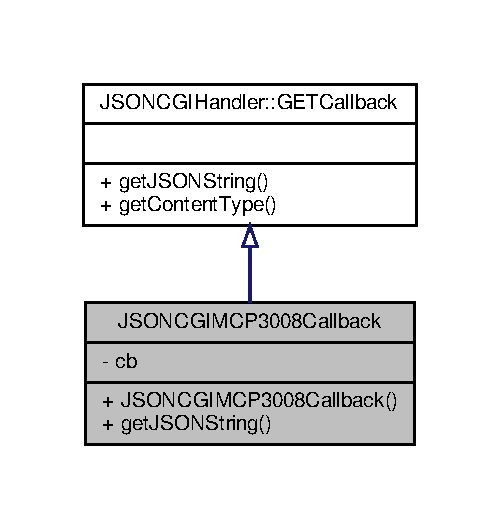
\includegraphics[width=240pt]{classJSONCGIMCP3008Callback__inherit__graph}
\end{center}
\end{figure}


Collaboration diagram for J\+S\+O\+N\+C\+G\+I\+M\+C\+P3008\+Callback\+:
\nopagebreak
\begin{figure}[H]
\begin{center}
\leavevmode
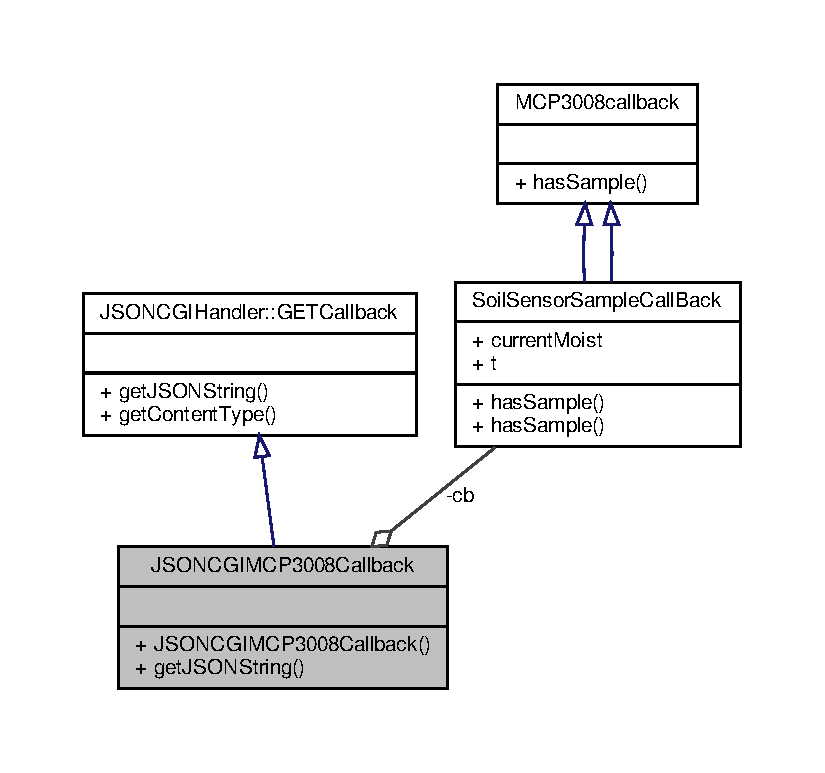
\includegraphics[width=350pt]{classJSONCGIMCP3008Callback__coll__graph}
\end{center}
\end{figure}
\subsection*{Public Member Functions}
\begin{DoxyCompactItemize}
\item 
\hyperlink{classJSONCGIMCP3008Callback_aa90aec09ae3eadaf9834ae3aad22a505}{J\+S\+O\+N\+C\+G\+I\+M\+C\+P3008\+Callback} (\hyperlink{classSoilSensorSampleCallBack}{Soil\+Sensor\+Sample\+Call\+Back} $\ast$s)
\item 
virtual std\+::string \hyperlink{classJSONCGIMCP3008Callback_aac6e6543d0b4da62f72781f3fe47ebed}{get\+J\+S\+O\+N\+String} ()
\end{DoxyCompactItemize}
\subsection*{Private Attributes}
\begin{DoxyCompactItemize}
\item 
\hyperlink{classSoilSensorSampleCallBack}{Soil\+Sensor\+Sample\+Call\+Back} $\ast$ \hyperlink{classJSONCGIMCP3008Callback_a2bfea06cf990c5ed9b3d2180a8c9996e}{cb}
\end{DoxyCompactItemize}


\subsection{Detailed Description}
Callback handler which returns data to the nginx server. The current soil moisture and the timestamp is transmitted to nginx and the javascript application. 

\subsection{Constructor \& Destructor Documentation}
\mbox{\Hypertarget{classJSONCGIMCP3008Callback_aa90aec09ae3eadaf9834ae3aad22a505}\label{classJSONCGIMCP3008Callback_aa90aec09ae3eadaf9834ae3aad22a505}} 
\index{J\+S\+O\+N\+C\+G\+I\+M\+C\+P3008\+Callback@{J\+S\+O\+N\+C\+G\+I\+M\+C\+P3008\+Callback}!J\+S\+O\+N\+C\+G\+I\+M\+C\+P3008\+Callback@{J\+S\+O\+N\+C\+G\+I\+M\+C\+P3008\+Callback}}
\index{J\+S\+O\+N\+C\+G\+I\+M\+C\+P3008\+Callback@{J\+S\+O\+N\+C\+G\+I\+M\+C\+P3008\+Callback}!J\+S\+O\+N\+C\+G\+I\+M\+C\+P3008\+Callback@{J\+S\+O\+N\+C\+G\+I\+M\+C\+P3008\+Callback}}
\subsubsection{\texorpdfstring{J\+S\+O\+N\+C\+G\+I\+M\+C\+P3008\+Callback()}{JSONCGIMCP3008Callback()}}
{\footnotesize\ttfamily J\+S\+O\+N\+C\+G\+I\+M\+C\+P3008\+Callback\+::\+J\+S\+O\+N\+C\+G\+I\+M\+C\+P3008\+Callback (\begin{DoxyParamCaption}\item[{\hyperlink{classSoilSensorSampleCallBack}{Soil\+Sensor\+Sample\+Call\+Back} $\ast$}]{s }\end{DoxyParamCaption})\hspace{0.3cm}{\ttfamily [inline]}}



\subsection{Member Function Documentation}
\mbox{\Hypertarget{classJSONCGIMCP3008Callback_aac6e6543d0b4da62f72781f3fe47ebed}\label{classJSONCGIMCP3008Callback_aac6e6543d0b4da62f72781f3fe47ebed}} 
\index{J\+S\+O\+N\+C\+G\+I\+M\+C\+P3008\+Callback@{J\+S\+O\+N\+C\+G\+I\+M\+C\+P3008\+Callback}!get\+J\+S\+O\+N\+String@{get\+J\+S\+O\+N\+String}}
\index{get\+J\+S\+O\+N\+String@{get\+J\+S\+O\+N\+String}!J\+S\+O\+N\+C\+G\+I\+M\+C\+P3008\+Callback@{J\+S\+O\+N\+C\+G\+I\+M\+C\+P3008\+Callback}}
\subsubsection{\texorpdfstring{get\+J\+S\+O\+N\+String()}{getJSONString()}}
{\footnotesize\ttfamily virtual std\+::string J\+S\+O\+N\+C\+G\+I\+M\+C\+P3008\+Callback\+::get\+J\+S\+O\+N\+String (\begin{DoxyParamCaption}{ }\end{DoxyParamCaption})\hspace{0.3cm}{\ttfamily [inline]}, {\ttfamily [virtual]}}

Needs to return the payload data sent to the web browser. Use the J\+S\+O\+N\+Generator to create the J\+S\+ON or use an external json generator. \begin{DoxyReturn}{Returns}
J\+S\+ON data 
\end{DoxyReturn}


Implements \hyperlink{classJSONCGIHandler_1_1GETCallback_a2367bf5a5912e9e5599ee464e0846255}{J\+S\+O\+N\+C\+G\+I\+Handler\+::\+G\+E\+T\+Callback}.

Here is the call graph for this function\+:
\nopagebreak
\begin{figure}[H]
\begin{center}
\leavevmode
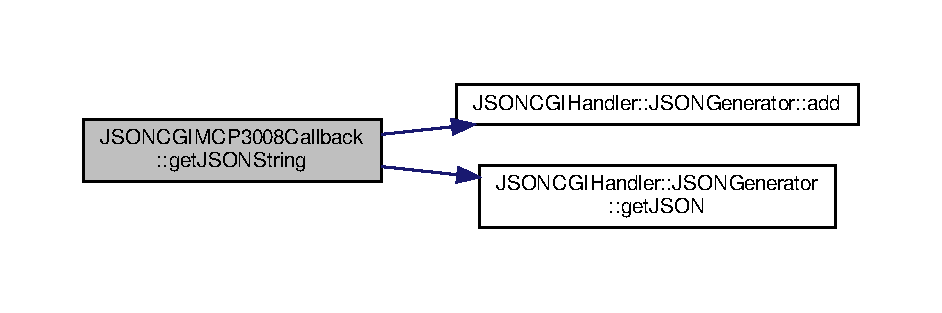
\includegraphics[width=350pt]{classJSONCGIMCP3008Callback_aac6e6543d0b4da62f72781f3fe47ebed_cgraph}
\end{center}
\end{figure}


\subsection{Field Documentation}
\mbox{\Hypertarget{classJSONCGIMCP3008Callback_a2bfea06cf990c5ed9b3d2180a8c9996e}\label{classJSONCGIMCP3008Callback_a2bfea06cf990c5ed9b3d2180a8c9996e}} 
\index{J\+S\+O\+N\+C\+G\+I\+M\+C\+P3008\+Callback@{J\+S\+O\+N\+C\+G\+I\+M\+C\+P3008\+Callback}!cb@{cb}}
\index{cb@{cb}!J\+S\+O\+N\+C\+G\+I\+M\+C\+P3008\+Callback@{J\+S\+O\+N\+C\+G\+I\+M\+C\+P3008\+Callback}}
\subsubsection{\texorpdfstring{cb}{cb}}
{\footnotesize\ttfamily \hyperlink{classSoilSensorSampleCallBack}{Soil\+Sensor\+Sample\+Call\+Back}$\ast$ J\+S\+O\+N\+C\+G\+I\+M\+C\+P3008\+Callback\+::cb\hspace{0.3cm}{\ttfamily [private]}}



The documentation for this class was generated from the following file\+:\begin{DoxyCompactItemize}
\item 
src/\hyperlink{main_8cpp}{main.\+cpp}\end{DoxyCompactItemize}

\hypertarget{classJSONDHT11CallbackHum}{}\section{J\+S\+O\+N\+D\+H\+T11\+Callback\+Hum Class Reference}
\label{classJSONDHT11CallbackHum}\index{J\+S\+O\+N\+D\+H\+T11\+Callback\+Hum@{J\+S\+O\+N\+D\+H\+T11\+Callback\+Hum}}


Inheritance diagram for J\+S\+O\+N\+D\+H\+T11\+Callback\+Hum\+:
\nopagebreak
\begin{figure}[H]
\begin{center}
\leavevmode
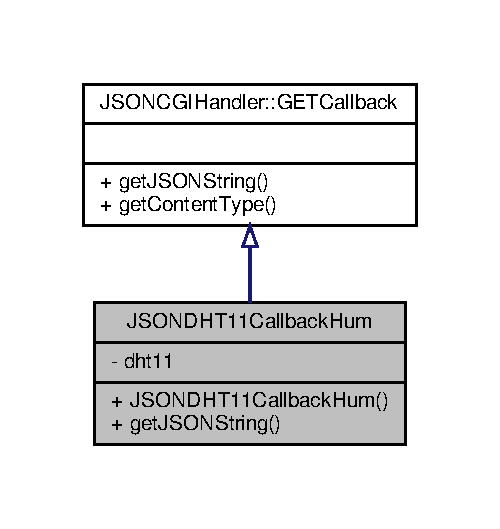
\includegraphics[width=240pt]{classJSONDHT11CallbackHum__inherit__graph}
\end{center}
\end{figure}


Collaboration diagram for J\+S\+O\+N\+D\+H\+T11\+Callback\+Hum\+:
\nopagebreak
\begin{figure}[H]
\begin{center}
\leavevmode
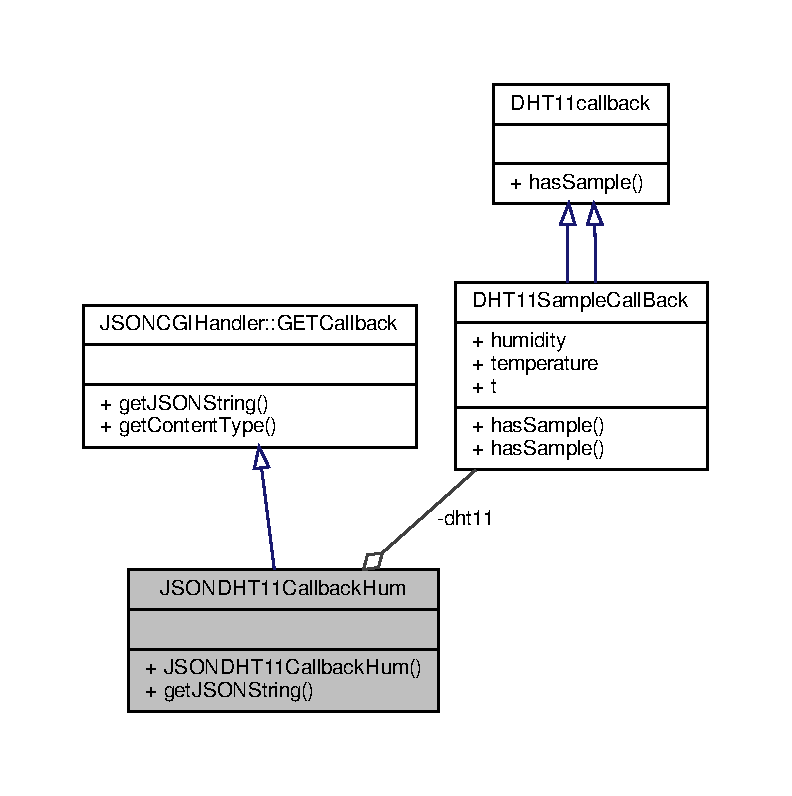
\includegraphics[width=350pt]{classJSONDHT11CallbackHum__coll__graph}
\end{center}
\end{figure}
\subsection*{Public Member Functions}
\begin{DoxyCompactItemize}
\item 
\hyperlink{classJSONDHT11CallbackHum_a618950489c3876213fbf842a28160cbb}{J\+S\+O\+N\+D\+H\+T11\+Callback\+Hum} (\hyperlink{classDHT11SampleCallBack}{D\+H\+T11\+Sample\+Call\+Back} $\ast$cb)
\item 
virtual std\+::string \hyperlink{classJSONDHT11CallbackHum_acc4cc41772967e063e1364d7c92ab985}{get\+J\+S\+O\+N\+String} ()
\end{DoxyCompactItemize}
\subsection*{Private Attributes}
\begin{DoxyCompactItemize}
\item 
\hyperlink{classDHT11SampleCallBack}{D\+H\+T11\+Sample\+Call\+Back} $\ast$ \hyperlink{classJSONDHT11CallbackHum_a6f4b2f8203acb357b5f01163f5cb76d8}{dht11}
\end{DoxyCompactItemize}


\subsection{Detailed Description}
Callback handler which returns data to the nginx server. The current humidity and the timestamp is transmitted to nginx and the javascript application. 

\subsection{Constructor \& Destructor Documentation}
\mbox{\Hypertarget{classJSONDHT11CallbackHum_a618950489c3876213fbf842a28160cbb}\label{classJSONDHT11CallbackHum_a618950489c3876213fbf842a28160cbb}} 
\index{J\+S\+O\+N\+D\+H\+T11\+Callback\+Hum@{J\+S\+O\+N\+D\+H\+T11\+Callback\+Hum}!J\+S\+O\+N\+D\+H\+T11\+Callback\+Hum@{J\+S\+O\+N\+D\+H\+T11\+Callback\+Hum}}
\index{J\+S\+O\+N\+D\+H\+T11\+Callback\+Hum@{J\+S\+O\+N\+D\+H\+T11\+Callback\+Hum}!J\+S\+O\+N\+D\+H\+T11\+Callback\+Hum@{J\+S\+O\+N\+D\+H\+T11\+Callback\+Hum}}
\subsubsection{\texorpdfstring{J\+S\+O\+N\+D\+H\+T11\+Callback\+Hum()}{JSONDHT11CallbackHum()}}
{\footnotesize\ttfamily J\+S\+O\+N\+D\+H\+T11\+Callback\+Hum\+::\+J\+S\+O\+N\+D\+H\+T11\+Callback\+Hum (\begin{DoxyParamCaption}\item[{\hyperlink{classDHT11SampleCallBack}{D\+H\+T11\+Sample\+Call\+Back} $\ast$}]{cb }\end{DoxyParamCaption})\hspace{0.3cm}{\ttfamily [inline]}}



\subsection{Member Function Documentation}
\mbox{\Hypertarget{classJSONDHT11CallbackHum_acc4cc41772967e063e1364d7c92ab985}\label{classJSONDHT11CallbackHum_acc4cc41772967e063e1364d7c92ab985}} 
\index{J\+S\+O\+N\+D\+H\+T11\+Callback\+Hum@{J\+S\+O\+N\+D\+H\+T11\+Callback\+Hum}!get\+J\+S\+O\+N\+String@{get\+J\+S\+O\+N\+String}}
\index{get\+J\+S\+O\+N\+String@{get\+J\+S\+O\+N\+String}!J\+S\+O\+N\+D\+H\+T11\+Callback\+Hum@{J\+S\+O\+N\+D\+H\+T11\+Callback\+Hum}}
\subsubsection{\texorpdfstring{get\+J\+S\+O\+N\+String()}{getJSONString()}}
{\footnotesize\ttfamily virtual std\+::string J\+S\+O\+N\+D\+H\+T11\+Callback\+Hum\+::get\+J\+S\+O\+N\+String (\begin{DoxyParamCaption}{ }\end{DoxyParamCaption})\hspace{0.3cm}{\ttfamily [inline]}, {\ttfamily [virtual]}}

Needs to return the payload data sent to the web browser. Use the J\+S\+O\+N\+Generator to create the J\+S\+ON or use an external json generator. \begin{DoxyReturn}{Returns}
J\+S\+ON data 
\end{DoxyReturn}


Implements \hyperlink{classJSONCGIHandler_1_1GETCallback_a2367bf5a5912e9e5599ee464e0846255}{J\+S\+O\+N\+C\+G\+I\+Handler\+::\+G\+E\+T\+Callback}.

Here is the call graph for this function\+:
\nopagebreak
\begin{figure}[H]
\begin{center}
\leavevmode
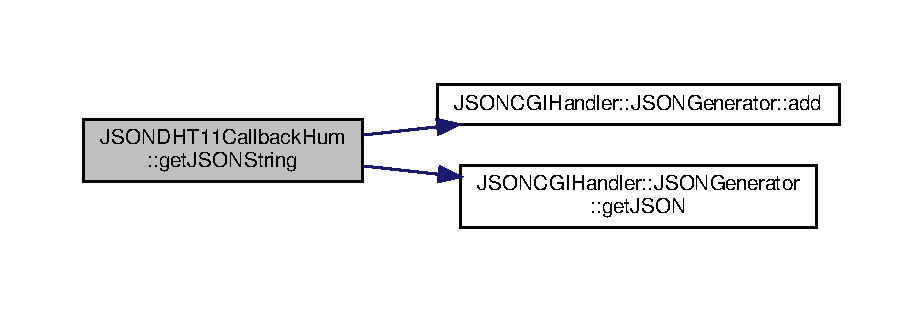
\includegraphics[width=350pt]{classJSONDHT11CallbackHum_acc4cc41772967e063e1364d7c92ab985_cgraph}
\end{center}
\end{figure}


\subsection{Field Documentation}
\mbox{\Hypertarget{classJSONDHT11CallbackHum_a6f4b2f8203acb357b5f01163f5cb76d8}\label{classJSONDHT11CallbackHum_a6f4b2f8203acb357b5f01163f5cb76d8}} 
\index{J\+S\+O\+N\+D\+H\+T11\+Callback\+Hum@{J\+S\+O\+N\+D\+H\+T11\+Callback\+Hum}!dht11@{dht11}}
\index{dht11@{dht11}!J\+S\+O\+N\+D\+H\+T11\+Callback\+Hum@{J\+S\+O\+N\+D\+H\+T11\+Callback\+Hum}}
\subsubsection{\texorpdfstring{dht11}{dht11}}
{\footnotesize\ttfamily \hyperlink{classDHT11SampleCallBack}{D\+H\+T11\+Sample\+Call\+Back}$\ast$ J\+S\+O\+N\+D\+H\+T11\+Callback\+Hum\+::dht11\hspace{0.3cm}{\ttfamily [private]}}



The documentation for this class was generated from the following file\+:\begin{DoxyCompactItemize}
\item 
src/\hyperlink{main_8cpp}{main.\+cpp}\end{DoxyCompactItemize}

\hypertarget{classJSONDHT11CallbackTemp}{}\section{J\+S\+O\+N\+D\+H\+T11\+Callback\+Temp Class Reference}
\label{classJSONDHT11CallbackTemp}\index{J\+S\+O\+N\+D\+H\+T11\+Callback\+Temp@{J\+S\+O\+N\+D\+H\+T11\+Callback\+Temp}}


Inheritance diagram for J\+S\+O\+N\+D\+H\+T11\+Callback\+Temp\+:
\nopagebreak
\begin{figure}[H]
\begin{center}
\leavevmode
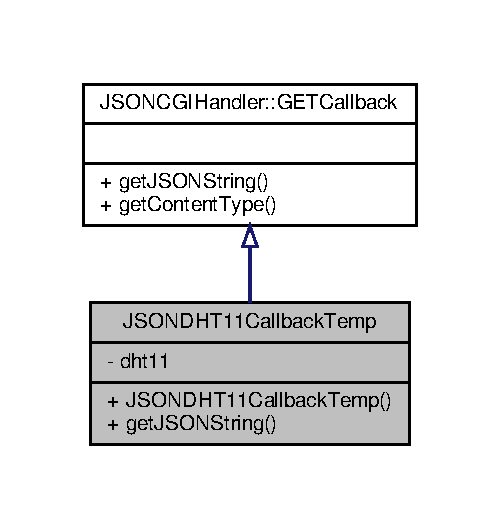
\includegraphics[width=240pt]{classJSONDHT11CallbackTemp__inherit__graph}
\end{center}
\end{figure}


Collaboration diagram for J\+S\+O\+N\+D\+H\+T11\+Callback\+Temp\+:
\nopagebreak
\begin{figure}[H]
\begin{center}
\leavevmode
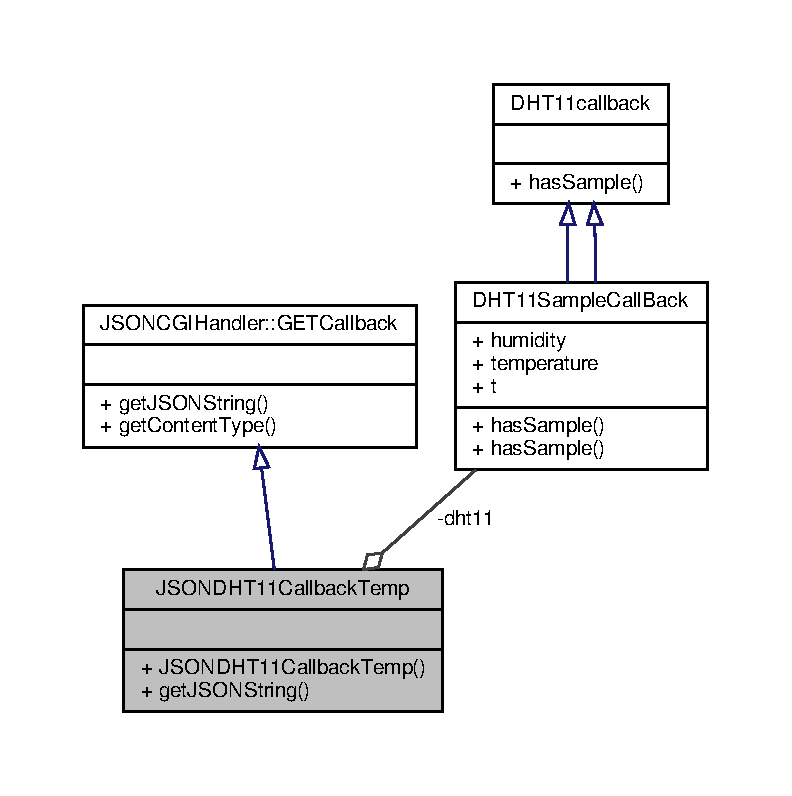
\includegraphics[width=350pt]{classJSONDHT11CallbackTemp__coll__graph}
\end{center}
\end{figure}
\subsection*{Public Member Functions}
\begin{DoxyCompactItemize}
\item 
\hyperlink{classJSONDHT11CallbackTemp_a53d61d27b86356366484b55973182cda}{J\+S\+O\+N\+D\+H\+T11\+Callback\+Temp} (\hyperlink{classDHT11SampleCallBack}{D\+H\+T11\+Sample\+Call\+Back} $\ast$cb)
\item 
virtual std\+::string \hyperlink{classJSONDHT11CallbackTemp_afe3fed3115bf659bdeb92463c7965dac}{get\+J\+S\+O\+N\+String} ()
\end{DoxyCompactItemize}
\subsection*{Private Attributes}
\begin{DoxyCompactItemize}
\item 
\hyperlink{classDHT11SampleCallBack}{D\+H\+T11\+Sample\+Call\+Back} $\ast$ \hyperlink{classJSONDHT11CallbackTemp_aed9fd605ded1a4cf2b9d5b4bdf5071be}{dht11}
\end{DoxyCompactItemize}


\subsection{Detailed Description}
Callback handler which returns data to the nginx server. The current temperature and the timestamp is transmitted to nginx and the javascript application. 

\subsection{Constructor \& Destructor Documentation}
\mbox{\Hypertarget{classJSONDHT11CallbackTemp_a53d61d27b86356366484b55973182cda}\label{classJSONDHT11CallbackTemp_a53d61d27b86356366484b55973182cda}} 
\index{J\+S\+O\+N\+D\+H\+T11\+Callback\+Temp@{J\+S\+O\+N\+D\+H\+T11\+Callback\+Temp}!J\+S\+O\+N\+D\+H\+T11\+Callback\+Temp@{J\+S\+O\+N\+D\+H\+T11\+Callback\+Temp}}
\index{J\+S\+O\+N\+D\+H\+T11\+Callback\+Temp@{J\+S\+O\+N\+D\+H\+T11\+Callback\+Temp}!J\+S\+O\+N\+D\+H\+T11\+Callback\+Temp@{J\+S\+O\+N\+D\+H\+T11\+Callback\+Temp}}
\subsubsection{\texorpdfstring{J\+S\+O\+N\+D\+H\+T11\+Callback\+Temp()}{JSONDHT11CallbackTemp()}}
{\footnotesize\ttfamily J\+S\+O\+N\+D\+H\+T11\+Callback\+Temp\+::\+J\+S\+O\+N\+D\+H\+T11\+Callback\+Temp (\begin{DoxyParamCaption}\item[{\hyperlink{classDHT11SampleCallBack}{D\+H\+T11\+Sample\+Call\+Back} $\ast$}]{cb }\end{DoxyParamCaption})\hspace{0.3cm}{\ttfamily [inline]}}



\subsection{Member Function Documentation}
\mbox{\Hypertarget{classJSONDHT11CallbackTemp_afe3fed3115bf659bdeb92463c7965dac}\label{classJSONDHT11CallbackTemp_afe3fed3115bf659bdeb92463c7965dac}} 
\index{J\+S\+O\+N\+D\+H\+T11\+Callback\+Temp@{J\+S\+O\+N\+D\+H\+T11\+Callback\+Temp}!get\+J\+S\+O\+N\+String@{get\+J\+S\+O\+N\+String}}
\index{get\+J\+S\+O\+N\+String@{get\+J\+S\+O\+N\+String}!J\+S\+O\+N\+D\+H\+T11\+Callback\+Temp@{J\+S\+O\+N\+D\+H\+T11\+Callback\+Temp}}
\subsubsection{\texorpdfstring{get\+J\+S\+O\+N\+String()}{getJSONString()}}
{\footnotesize\ttfamily virtual std\+::string J\+S\+O\+N\+D\+H\+T11\+Callback\+Temp\+::get\+J\+S\+O\+N\+String (\begin{DoxyParamCaption}{ }\end{DoxyParamCaption})\hspace{0.3cm}{\ttfamily [inline]}, {\ttfamily [virtual]}}

Needs to return the payload data sent to the web browser. Use the J\+S\+O\+N\+Generator to create the J\+S\+ON or use an external json generator. \begin{DoxyReturn}{Returns}
J\+S\+ON data 
\end{DoxyReturn}


Implements \hyperlink{classJSONCGIHandler_1_1GETCallback_a2367bf5a5912e9e5599ee464e0846255}{J\+S\+O\+N\+C\+G\+I\+Handler\+::\+G\+E\+T\+Callback}.

Here is the call graph for this function\+:
\nopagebreak
\begin{figure}[H]
\begin{center}
\leavevmode
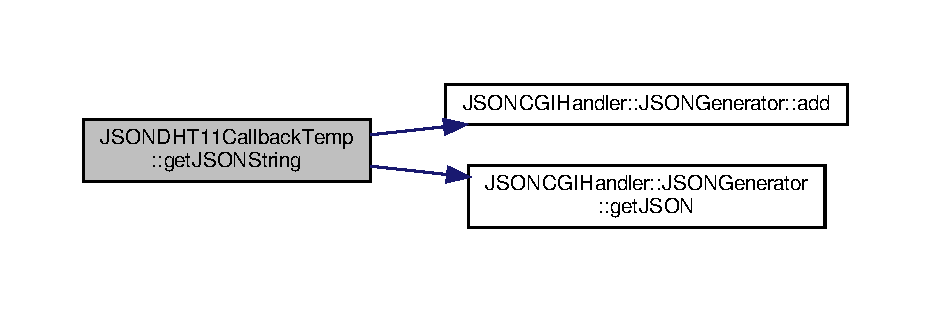
\includegraphics[width=350pt]{classJSONDHT11CallbackTemp_afe3fed3115bf659bdeb92463c7965dac_cgraph}
\end{center}
\end{figure}


\subsection{Field Documentation}
\mbox{\Hypertarget{classJSONDHT11CallbackTemp_aed9fd605ded1a4cf2b9d5b4bdf5071be}\label{classJSONDHT11CallbackTemp_aed9fd605ded1a4cf2b9d5b4bdf5071be}} 
\index{J\+S\+O\+N\+D\+H\+T11\+Callback\+Temp@{J\+S\+O\+N\+D\+H\+T11\+Callback\+Temp}!dht11@{dht11}}
\index{dht11@{dht11}!J\+S\+O\+N\+D\+H\+T11\+Callback\+Temp@{J\+S\+O\+N\+D\+H\+T11\+Callback\+Temp}}
\subsubsection{\texorpdfstring{dht11}{dht11}}
{\footnotesize\ttfamily \hyperlink{classDHT11SampleCallBack}{D\+H\+T11\+Sample\+Call\+Back}$\ast$ J\+S\+O\+N\+D\+H\+T11\+Callback\+Temp\+::dht11\hspace{0.3cm}{\ttfamily [private]}}



The documentation for this class was generated from the following file\+:\begin{DoxyCompactItemize}
\item 
src/\hyperlink{main_8cpp}{main.\+cpp}\end{DoxyCompactItemize}

\hypertarget{classJSONCGIHandler_1_1JSONGenerator}{}\section{J\+S\+O\+N\+C\+G\+I\+Handler\+:\+:J\+S\+O\+N\+Generator Class Reference}
\label{classJSONCGIHandler_1_1JSONGenerator}\index{J\+S\+O\+N\+C\+G\+I\+Handler\+::\+J\+S\+O\+N\+Generator@{J\+S\+O\+N\+C\+G\+I\+Handler\+::\+J\+S\+O\+N\+Generator}}


{\ttfamily \#include $<$json\+\_\+fastcgi\+\_\+web\+\_\+api.\+h$>$}



Collaboration diagram for J\+S\+O\+N\+C\+G\+I\+Handler\+:\+:J\+S\+O\+N\+Generator\+:
\nopagebreak
\begin{figure}[H]
\begin{center}
\leavevmode
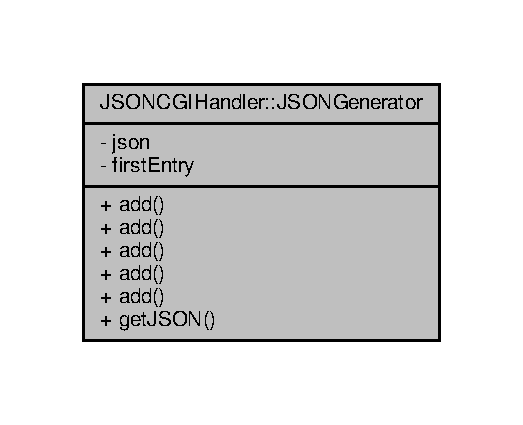
\includegraphics[width=251pt]{classJSONCGIHandler_1_1JSONGenerator__coll__graph}
\end{center}
\end{figure}
\subsection*{Public Member Functions}
\begin{DoxyCompactItemize}
\item 
void \hyperlink{classJSONCGIHandler_1_1JSONGenerator_a191efd00967cbace0d9ddfedea39cd9b}{add} (std\+::string key, std\+::string value)
\item 
void \hyperlink{classJSONCGIHandler_1_1JSONGenerator_aa25099deb2442335298ab1c021f36910}{add} (std\+::string key, double value)
\item 
void \hyperlink{classJSONCGIHandler_1_1JSONGenerator_a2192849b22341653a138bb63da6c6c9a}{add} (std\+::string key, float value)
\item 
void \hyperlink{classJSONCGIHandler_1_1JSONGenerator_afc3e9374b0e49ca1f701bd22bbd4cd92}{add} (std\+::string key, long value)
\item 
void \hyperlink{classJSONCGIHandler_1_1JSONGenerator_a87fe5c75b46f9822255535a61f15ad4b}{add} (std\+::string key, int value)
\item 
std\+::string \hyperlink{classJSONCGIHandler_1_1JSONGenerator_afec28cd80e562955e2cd8cdb92d86205}{get\+J\+S\+ON} ()
\end{DoxyCompactItemize}
\subsection*{Private Attributes}
\begin{DoxyCompactItemize}
\item 
std\+::string \hyperlink{classJSONCGIHandler_1_1JSONGenerator_a5a9fd42e7b9030c6a0a4bee923a2e416}{json} = \char`\"{}\{\char`\"{}
\item 
int \hyperlink{classJSONCGIHandler_1_1JSONGenerator_a9d14c80af92fa9f3a3406d826acd2cc0}{first\+Entry} = 1
\end{DoxyCompactItemize}


\subsection{Detailed Description}
Simple helper function to create a key/value json pairs for the callback function. 

\subsection{Member Function Documentation}
\mbox{\Hypertarget{classJSONCGIHandler_1_1JSONGenerator_a191efd00967cbace0d9ddfedea39cd9b}\label{classJSONCGIHandler_1_1JSONGenerator_a191efd00967cbace0d9ddfedea39cd9b}} 
\index{J\+S\+O\+N\+C\+G\+I\+Handler\+::\+J\+S\+O\+N\+Generator@{J\+S\+O\+N\+C\+G\+I\+Handler\+::\+J\+S\+O\+N\+Generator}!add@{add}}
\index{add@{add}!J\+S\+O\+N\+C\+G\+I\+Handler\+::\+J\+S\+O\+N\+Generator@{J\+S\+O\+N\+C\+G\+I\+Handler\+::\+J\+S\+O\+N\+Generator}}
\subsubsection{\texorpdfstring{add()}{add()}\hspace{0.1cm}{\footnotesize\ttfamily [1/5]}}
{\footnotesize\ttfamily void J\+S\+O\+N\+C\+G\+I\+Handler\+::\+J\+S\+O\+N\+Generator\+::add (\begin{DoxyParamCaption}\item[{std\+::string}]{key,  }\item[{std\+::string}]{value }\end{DoxyParamCaption})\hspace{0.3cm}{\ttfamily [inline]}}

Adds a J\+S\+ON entry\+: string 
\begin{DoxyParams}{Parameters}
{\em key} & The J\+S\+ON key \\
\hline
{\em value} & The J\+S\+ON value as a string \\
\hline
\end{DoxyParams}
Here is the caller graph for this function\+:
\nopagebreak
\begin{figure}[H]
\begin{center}
\leavevmode
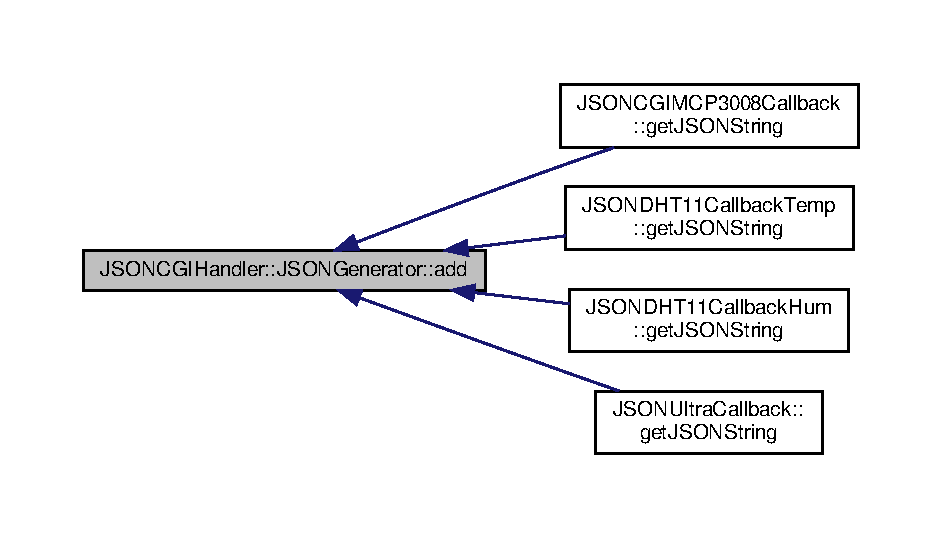
\includegraphics[width=350pt]{classJSONCGIHandler_1_1JSONGenerator_a191efd00967cbace0d9ddfedea39cd9b_icgraph}
\end{center}
\end{figure}
\mbox{\Hypertarget{classJSONCGIHandler_1_1JSONGenerator_aa25099deb2442335298ab1c021f36910}\label{classJSONCGIHandler_1_1JSONGenerator_aa25099deb2442335298ab1c021f36910}} 
\index{J\+S\+O\+N\+C\+G\+I\+Handler\+::\+J\+S\+O\+N\+Generator@{J\+S\+O\+N\+C\+G\+I\+Handler\+::\+J\+S\+O\+N\+Generator}!add@{add}}
\index{add@{add}!J\+S\+O\+N\+C\+G\+I\+Handler\+::\+J\+S\+O\+N\+Generator@{J\+S\+O\+N\+C\+G\+I\+Handler\+::\+J\+S\+O\+N\+Generator}}
\subsubsection{\texorpdfstring{add()}{add()}\hspace{0.1cm}{\footnotesize\ttfamily [2/5]}}
{\footnotesize\ttfamily void J\+S\+O\+N\+C\+G\+I\+Handler\+::\+J\+S\+O\+N\+Generator\+::add (\begin{DoxyParamCaption}\item[{std\+::string}]{key,  }\item[{double}]{value }\end{DoxyParamCaption})\hspace{0.3cm}{\ttfamily [inline]}}

Adds a J\+S\+ON entry\+: double 
\begin{DoxyParams}{Parameters}
{\em key} & The J\+S\+ON key \\
\hline
{\em value} & The J\+S\+ON value as a double \\
\hline
\end{DoxyParams}
\mbox{\Hypertarget{classJSONCGIHandler_1_1JSONGenerator_a2192849b22341653a138bb63da6c6c9a}\label{classJSONCGIHandler_1_1JSONGenerator_a2192849b22341653a138bb63da6c6c9a}} 
\index{J\+S\+O\+N\+C\+G\+I\+Handler\+::\+J\+S\+O\+N\+Generator@{J\+S\+O\+N\+C\+G\+I\+Handler\+::\+J\+S\+O\+N\+Generator}!add@{add}}
\index{add@{add}!J\+S\+O\+N\+C\+G\+I\+Handler\+::\+J\+S\+O\+N\+Generator@{J\+S\+O\+N\+C\+G\+I\+Handler\+::\+J\+S\+O\+N\+Generator}}
\subsubsection{\texorpdfstring{add()}{add()}\hspace{0.1cm}{\footnotesize\ttfamily [3/5]}}
{\footnotesize\ttfamily void J\+S\+O\+N\+C\+G\+I\+Handler\+::\+J\+S\+O\+N\+Generator\+::add (\begin{DoxyParamCaption}\item[{std\+::string}]{key,  }\item[{float}]{value }\end{DoxyParamCaption})\hspace{0.3cm}{\ttfamily [inline]}}

Adds a J\+S\+ON entry\+: float 
\begin{DoxyParams}{Parameters}
{\em key} & The J\+S\+ON key \\
\hline
{\em value} & The J\+S\+ON value as a float \\
\hline
\end{DoxyParams}
\mbox{\Hypertarget{classJSONCGIHandler_1_1JSONGenerator_afc3e9374b0e49ca1f701bd22bbd4cd92}\label{classJSONCGIHandler_1_1JSONGenerator_afc3e9374b0e49ca1f701bd22bbd4cd92}} 
\index{J\+S\+O\+N\+C\+G\+I\+Handler\+::\+J\+S\+O\+N\+Generator@{J\+S\+O\+N\+C\+G\+I\+Handler\+::\+J\+S\+O\+N\+Generator}!add@{add}}
\index{add@{add}!J\+S\+O\+N\+C\+G\+I\+Handler\+::\+J\+S\+O\+N\+Generator@{J\+S\+O\+N\+C\+G\+I\+Handler\+::\+J\+S\+O\+N\+Generator}}
\subsubsection{\texorpdfstring{add()}{add()}\hspace{0.1cm}{\footnotesize\ttfamily [4/5]}}
{\footnotesize\ttfamily void J\+S\+O\+N\+C\+G\+I\+Handler\+::\+J\+S\+O\+N\+Generator\+::add (\begin{DoxyParamCaption}\item[{std\+::string}]{key,  }\item[{long}]{value }\end{DoxyParamCaption})\hspace{0.3cm}{\ttfamily [inline]}}

Adds a J\+S\+ON entry\+: long int 
\begin{DoxyParams}{Parameters}
{\em key} & The J\+S\+ON key \\
\hline
{\em value} & The J\+S\+ON value as a long int \\
\hline
\end{DoxyParams}
\mbox{\Hypertarget{classJSONCGIHandler_1_1JSONGenerator_a87fe5c75b46f9822255535a61f15ad4b}\label{classJSONCGIHandler_1_1JSONGenerator_a87fe5c75b46f9822255535a61f15ad4b}} 
\index{J\+S\+O\+N\+C\+G\+I\+Handler\+::\+J\+S\+O\+N\+Generator@{J\+S\+O\+N\+C\+G\+I\+Handler\+::\+J\+S\+O\+N\+Generator}!add@{add}}
\index{add@{add}!J\+S\+O\+N\+C\+G\+I\+Handler\+::\+J\+S\+O\+N\+Generator@{J\+S\+O\+N\+C\+G\+I\+Handler\+::\+J\+S\+O\+N\+Generator}}
\subsubsection{\texorpdfstring{add()}{add()}\hspace{0.1cm}{\footnotesize\ttfamily [5/5]}}
{\footnotesize\ttfamily void J\+S\+O\+N\+C\+G\+I\+Handler\+::\+J\+S\+O\+N\+Generator\+::add (\begin{DoxyParamCaption}\item[{std\+::string}]{key,  }\item[{int}]{value }\end{DoxyParamCaption})\hspace{0.3cm}{\ttfamily [inline]}}

Adds a J\+S\+ON entry\+: int 
\begin{DoxyParams}{Parameters}
{\em key} & The J\+S\+ON key \\
\hline
{\em value} & The J\+S\+ON value as an int \\
\hline
\end{DoxyParams}
\mbox{\Hypertarget{classJSONCGIHandler_1_1JSONGenerator_afec28cd80e562955e2cd8cdb92d86205}\label{classJSONCGIHandler_1_1JSONGenerator_afec28cd80e562955e2cd8cdb92d86205}} 
\index{J\+S\+O\+N\+C\+G\+I\+Handler\+::\+J\+S\+O\+N\+Generator@{J\+S\+O\+N\+C\+G\+I\+Handler\+::\+J\+S\+O\+N\+Generator}!get\+J\+S\+ON@{get\+J\+S\+ON}}
\index{get\+J\+S\+ON@{get\+J\+S\+ON}!J\+S\+O\+N\+C\+G\+I\+Handler\+::\+J\+S\+O\+N\+Generator@{J\+S\+O\+N\+C\+G\+I\+Handler\+::\+J\+S\+O\+N\+Generator}}
\subsubsection{\texorpdfstring{get\+J\+S\+O\+N()}{getJSON()}}
{\footnotesize\ttfamily std\+::string J\+S\+O\+N\+C\+G\+I\+Handler\+::\+J\+S\+O\+N\+Generator\+::get\+J\+S\+ON (\begin{DoxyParamCaption}{ }\end{DoxyParamCaption})\hspace{0.3cm}{\ttfamily [inline]}}

Gets the json string \begin{DoxyReturn}{Returns}
The J\+S\+ON data ready to be sent 
\end{DoxyReturn}
Here is the caller graph for this function\+:
\nopagebreak
\begin{figure}[H]
\begin{center}
\leavevmode
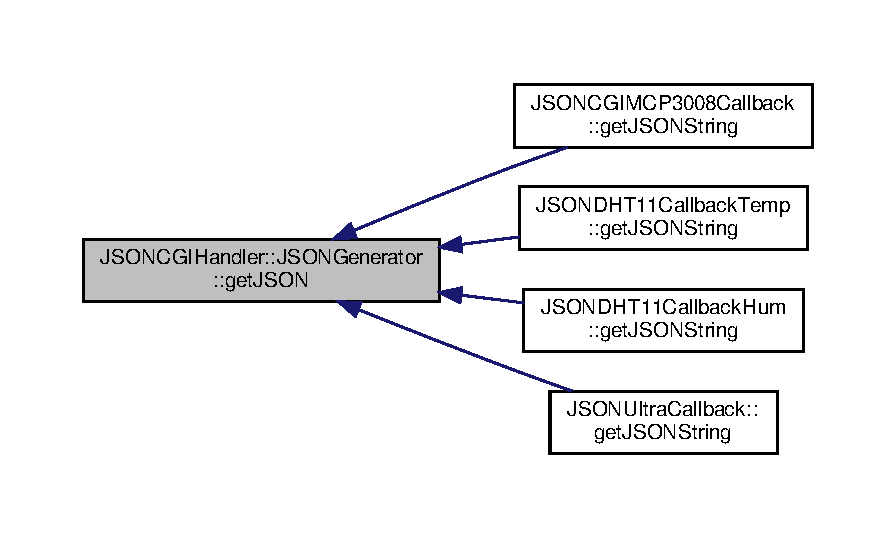
\includegraphics[width=350pt]{classJSONCGIHandler_1_1JSONGenerator_afec28cd80e562955e2cd8cdb92d86205_icgraph}
\end{center}
\end{figure}


\subsection{Field Documentation}
\mbox{\Hypertarget{classJSONCGIHandler_1_1JSONGenerator_a9d14c80af92fa9f3a3406d826acd2cc0}\label{classJSONCGIHandler_1_1JSONGenerator_a9d14c80af92fa9f3a3406d826acd2cc0}} 
\index{J\+S\+O\+N\+C\+G\+I\+Handler\+::\+J\+S\+O\+N\+Generator@{J\+S\+O\+N\+C\+G\+I\+Handler\+::\+J\+S\+O\+N\+Generator}!first\+Entry@{first\+Entry}}
\index{first\+Entry@{first\+Entry}!J\+S\+O\+N\+C\+G\+I\+Handler\+::\+J\+S\+O\+N\+Generator@{J\+S\+O\+N\+C\+G\+I\+Handler\+::\+J\+S\+O\+N\+Generator}}
\subsubsection{\texorpdfstring{first\+Entry}{firstEntry}}
{\footnotesize\ttfamily int J\+S\+O\+N\+C\+G\+I\+Handler\+::\+J\+S\+O\+N\+Generator\+::first\+Entry = 1\hspace{0.3cm}{\ttfamily [private]}}

\mbox{\Hypertarget{classJSONCGIHandler_1_1JSONGenerator_a5a9fd42e7b9030c6a0a4bee923a2e416}\label{classJSONCGIHandler_1_1JSONGenerator_a5a9fd42e7b9030c6a0a4bee923a2e416}} 
\index{J\+S\+O\+N\+C\+G\+I\+Handler\+::\+J\+S\+O\+N\+Generator@{J\+S\+O\+N\+C\+G\+I\+Handler\+::\+J\+S\+O\+N\+Generator}!json@{json}}
\index{json@{json}!J\+S\+O\+N\+C\+G\+I\+Handler\+::\+J\+S\+O\+N\+Generator@{J\+S\+O\+N\+C\+G\+I\+Handler\+::\+J\+S\+O\+N\+Generator}}
\subsubsection{\texorpdfstring{json}{json}}
{\footnotesize\ttfamily std\+::string J\+S\+O\+N\+C\+G\+I\+Handler\+::\+J\+S\+O\+N\+Generator\+::json = \char`\"{}\{\char`\"{}\hspace{0.3cm}{\ttfamily [private]}}



The documentation for this class was generated from the following file\+:\begin{DoxyCompactItemize}
\item 
src/\hyperlink{json__fastcgi__web__api_8h}{json\+\_\+fastcgi\+\_\+web\+\_\+api.\+h}\end{DoxyCompactItemize}

\hypertarget{classJSONUltraCallback}{}\section{J\+S\+O\+N\+Ultra\+Callback Class Reference}
\label{classJSONUltraCallback}\index{J\+S\+O\+N\+Ultra\+Callback@{J\+S\+O\+N\+Ultra\+Callback}}


Inheritance diagram for J\+S\+O\+N\+Ultra\+Callback\+:
\nopagebreak
\begin{figure}[H]
\begin{center}
\leavevmode
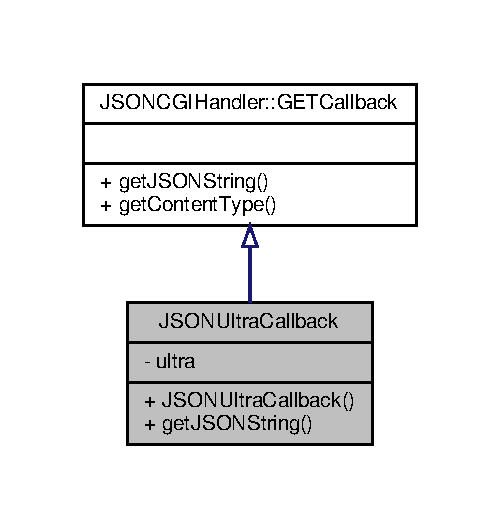
\includegraphics[width=240pt]{classJSONUltraCallback__inherit__graph}
\end{center}
\end{figure}


Collaboration diagram for J\+S\+O\+N\+Ultra\+Callback\+:
\nopagebreak
\begin{figure}[H]
\begin{center}
\leavevmode
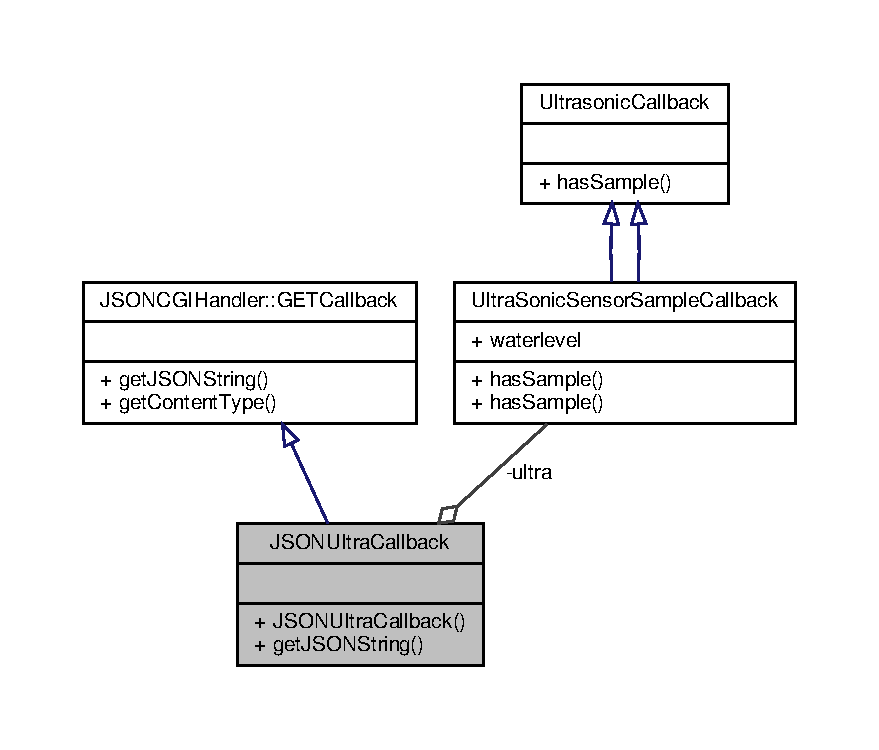
\includegraphics[width=350pt]{classJSONUltraCallback__coll__graph}
\end{center}
\end{figure}
\subsection*{Public Member Functions}
\begin{DoxyCompactItemize}
\item 
\hyperlink{classJSONUltraCallback_a3b9a7da41a3dc2b73abb3450fb2399e4}{J\+S\+O\+N\+Ultra\+Callback} (\hyperlink{classUltraSonicSensorSampleCallback}{Ultra\+Sonic\+Sensor\+Sample\+Callback} $\ast$cb)
\item 
virtual std\+::string \hyperlink{classJSONUltraCallback_abb097f82255b74c56370b90bc06d81da}{get\+J\+S\+O\+N\+String} ()
\end{DoxyCompactItemize}
\subsection*{Private Attributes}
\begin{DoxyCompactItemize}
\item 
\hyperlink{classUltraSonicSensorSampleCallback}{Ultra\+Sonic\+Sensor\+Sample\+Callback} $\ast$ \hyperlink{classJSONUltraCallback_aed520f877003033dff14d7bd636683dc}{ultra}
\end{DoxyCompactItemize}


\subsection{Detailed Description}
Callback handler which returns data to the nginx server. The current water level and the timestamp is transmitted to nginx and the javascript application. 

\subsection{Constructor \& Destructor Documentation}
\mbox{\Hypertarget{classJSONUltraCallback_a3b9a7da41a3dc2b73abb3450fb2399e4}\label{classJSONUltraCallback_a3b9a7da41a3dc2b73abb3450fb2399e4}} 
\index{J\+S\+O\+N\+Ultra\+Callback@{J\+S\+O\+N\+Ultra\+Callback}!J\+S\+O\+N\+Ultra\+Callback@{J\+S\+O\+N\+Ultra\+Callback}}
\index{J\+S\+O\+N\+Ultra\+Callback@{J\+S\+O\+N\+Ultra\+Callback}!J\+S\+O\+N\+Ultra\+Callback@{J\+S\+O\+N\+Ultra\+Callback}}
\subsubsection{\texorpdfstring{J\+S\+O\+N\+Ultra\+Callback()}{JSONUltraCallback()}}
{\footnotesize\ttfamily J\+S\+O\+N\+Ultra\+Callback\+::\+J\+S\+O\+N\+Ultra\+Callback (\begin{DoxyParamCaption}\item[{\hyperlink{classUltraSonicSensorSampleCallback}{Ultra\+Sonic\+Sensor\+Sample\+Callback} $\ast$}]{cb }\end{DoxyParamCaption})\hspace{0.3cm}{\ttfamily [inline]}}



\subsection{Member Function Documentation}
\mbox{\Hypertarget{classJSONUltraCallback_abb097f82255b74c56370b90bc06d81da}\label{classJSONUltraCallback_abb097f82255b74c56370b90bc06d81da}} 
\index{J\+S\+O\+N\+Ultra\+Callback@{J\+S\+O\+N\+Ultra\+Callback}!get\+J\+S\+O\+N\+String@{get\+J\+S\+O\+N\+String}}
\index{get\+J\+S\+O\+N\+String@{get\+J\+S\+O\+N\+String}!J\+S\+O\+N\+Ultra\+Callback@{J\+S\+O\+N\+Ultra\+Callback}}
\subsubsection{\texorpdfstring{get\+J\+S\+O\+N\+String()}{getJSONString()}}
{\footnotesize\ttfamily virtual std\+::string J\+S\+O\+N\+Ultra\+Callback\+::get\+J\+S\+O\+N\+String (\begin{DoxyParamCaption}{ }\end{DoxyParamCaption})\hspace{0.3cm}{\ttfamily [inline]}, {\ttfamily [virtual]}}

Needs to return the payload data sent to the web browser. Use the J\+S\+O\+N\+Generator to create the J\+S\+ON or use an external json generator. \begin{DoxyReturn}{Returns}
J\+S\+ON data 
\end{DoxyReturn}


Implements \hyperlink{classJSONCGIHandler_1_1GETCallback_a2367bf5a5912e9e5599ee464e0846255}{J\+S\+O\+N\+C\+G\+I\+Handler\+::\+G\+E\+T\+Callback}.

Here is the call graph for this function\+:
\nopagebreak
\begin{figure}[H]
\begin{center}
\leavevmode
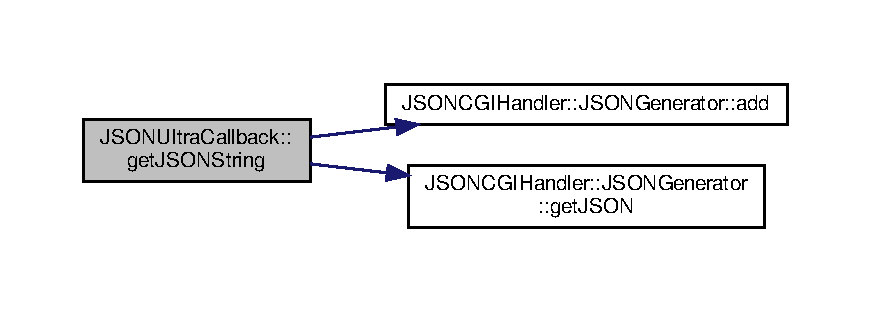
\includegraphics[width=350pt]{classJSONUltraCallback_abb097f82255b74c56370b90bc06d81da_cgraph}
\end{center}
\end{figure}


\subsection{Field Documentation}
\mbox{\Hypertarget{classJSONUltraCallback_aed520f877003033dff14d7bd636683dc}\label{classJSONUltraCallback_aed520f877003033dff14d7bd636683dc}} 
\index{J\+S\+O\+N\+Ultra\+Callback@{J\+S\+O\+N\+Ultra\+Callback}!ultra@{ultra}}
\index{ultra@{ultra}!J\+S\+O\+N\+Ultra\+Callback@{J\+S\+O\+N\+Ultra\+Callback}}
\subsubsection{\texorpdfstring{ultra}{ultra}}
{\footnotesize\ttfamily \hyperlink{classUltraSonicSensorSampleCallback}{Ultra\+Sonic\+Sensor\+Sample\+Callback}$\ast$ J\+S\+O\+N\+Ultra\+Callback\+::ultra\hspace{0.3cm}{\ttfamily [private]}}



The documentation for this class was generated from the following file\+:\begin{DoxyCompactItemize}
\item 
src/\hyperlink{main_8cpp}{main.\+cpp}\end{DoxyCompactItemize}

\hypertarget{classMCP3008}{}\section{M\+C\+P3008 Class Reference}
\label{classMCP3008}\index{M\+C\+P3008@{M\+C\+P3008}}


{\ttfamily \#include $<$M\+C\+P3008.\+h$>$}



Collaboration diagram for M\+C\+P3008\+:
\nopagebreak
\begin{figure}[H]
\begin{center}
\leavevmode
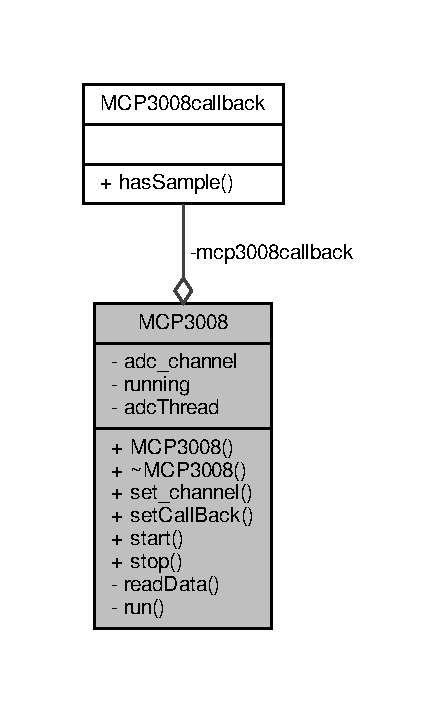
\includegraphics[width=210pt]{classMCP3008__coll__graph}
\end{center}
\end{figure}
\subsection*{Public Member Functions}
\begin{DoxyCompactItemize}
\item 
\hyperlink{classMCP3008_a31a9bfe04898e565154413cf17329859}{M\+C\+P3008} ()
\item 
\hyperlink{classMCP3008_a96d9ef77d32f0c4efd3b942c40322aeb}{$\sim$\+M\+C\+P3008} ()
\item 
void \hyperlink{classMCP3008_ad1893b9dd4dbbc2efbb57843871596fc}{set\+\_\+channel} (uint8\+\_\+t channel)
\item 
void \hyperlink{classMCP3008_abe098bf3c4c2e6a803c53297d84e3c1c}{set\+Call\+Back} (\hyperlink{classMCP3008callback}{M\+C\+P3008callback} $\ast$cb)
\item 
void \hyperlink{classMCP3008_a839bea8d430ee0852620c151c4467450}{start} ()
\item 
void \hyperlink{classMCP3008_add8fa4dafb68c227cd1ed269bd30603f}{stop} ()
\end{DoxyCompactItemize}
\subsection*{Private Member Functions}
\begin{DoxyCompactItemize}
\item 
int \hyperlink{classMCP3008_a583bf94e4bb38d945819914c9a2321ba}{read\+Data} ()
\end{DoxyCompactItemize}
\subsection*{Static Private Member Functions}
\begin{DoxyCompactItemize}
\item 
static void \hyperlink{classMCP3008_a8e243711492e50dd4327050ffae8851d}{run} (\hyperlink{classMCP3008}{M\+C\+P3008} $\ast$mcp3008)
\end{DoxyCompactItemize}
\subsection*{Private Attributes}
\begin{DoxyCompactItemize}
\item 
uint8\+\_\+t \hyperlink{classMCP3008_a9089ac2e245b158411670c802e6ea404}{adc\+\_\+channel}
\item 
\hyperlink{classMCP3008callback}{M\+C\+P3008callback} $\ast$ \hyperlink{classMCP3008_a602724521657fd93241ba51c8dd83e74}{mcp3008callback} = N\+U\+LL
\item 
int \hyperlink{classMCP3008_a81354e1933a79bcb9f1d01c0e16566f0}{running} = 0
\item 
std\+::thread $\ast$ \hyperlink{classMCP3008_ab1318bf3a8ac2bdf31b62451d29e1c90}{adc\+Thread} = N\+U\+LL
\end{DoxyCompactItemize}


\subsection{Detailed Description}
This class reads data from \hyperlink{classMCP3008}{M\+C\+P3008} A\+DC in the background and calls a callback whenever data is available 

\subsection{Constructor \& Destructor Documentation}
\mbox{\Hypertarget{classMCP3008_a31a9bfe04898e565154413cf17329859}\label{classMCP3008_a31a9bfe04898e565154413cf17329859}} 
\index{M\+C\+P3008@{M\+C\+P3008}!M\+C\+P3008@{M\+C\+P3008}}
\index{M\+C\+P3008@{M\+C\+P3008}!M\+C\+P3008@{M\+C\+P3008}}
\subsubsection{\texorpdfstring{M\+C\+P3008()}{MCP3008()}}
{\footnotesize\ttfamily M\+C\+P3008\+::\+M\+C\+P3008 (\begin{DoxyParamCaption}{ }\end{DoxyParamCaption})}

clas constructor \mbox{\Hypertarget{classMCP3008_a96d9ef77d32f0c4efd3b942c40322aeb}\label{classMCP3008_a96d9ef77d32f0c4efd3b942c40322aeb}} 
\index{M\+C\+P3008@{M\+C\+P3008}!````~M\+C\+P3008@{$\sim$\+M\+C\+P3008}}
\index{````~M\+C\+P3008@{$\sim$\+M\+C\+P3008}!M\+C\+P3008@{M\+C\+P3008}}
\subsubsection{\texorpdfstring{$\sim$\+M\+C\+P3008()}{~MCP3008()}}
{\footnotesize\ttfamily M\+C\+P3008\+::$\sim$\+M\+C\+P3008 (\begin{DoxyParamCaption}{ }\end{DoxyParamCaption})\hspace{0.3cm}{\ttfamily [inline]}}

clas destructor 

\subsection{Member Function Documentation}
\mbox{\Hypertarget{classMCP3008_a583bf94e4bb38d945819914c9a2321ba}\label{classMCP3008_a583bf94e4bb38d945819914c9a2321ba}} 
\index{M\+C\+P3008@{M\+C\+P3008}!read\+Data@{read\+Data}}
\index{read\+Data@{read\+Data}!M\+C\+P3008@{M\+C\+P3008}}
\subsubsection{\texorpdfstring{read\+Data()}{readData()}}
{\footnotesize\ttfamily int M\+C\+P3008\+::read\+Data (\begin{DoxyParamCaption}{ }\end{DoxyParamCaption})\hspace{0.3cm}{\ttfamily [private]}}

Here is the caller graph for this function\+:
\nopagebreak
\begin{figure}[H]
\begin{center}
\leavevmode
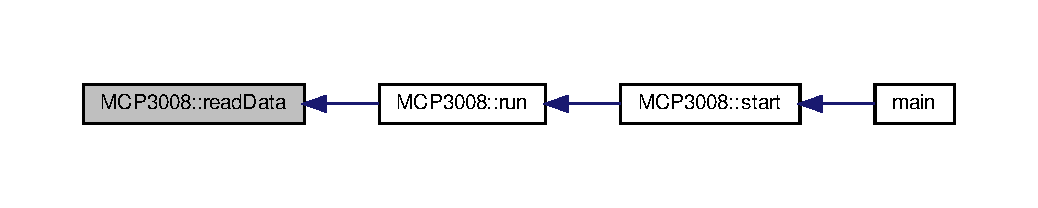
\includegraphics[width=350pt]{classMCP3008_a583bf94e4bb38d945819914c9a2321ba_icgraph}
\end{center}
\end{figure}
\mbox{\Hypertarget{classMCP3008_a8e243711492e50dd4327050ffae8851d}\label{classMCP3008_a8e243711492e50dd4327050ffae8851d}} 
\index{M\+C\+P3008@{M\+C\+P3008}!run@{run}}
\index{run@{run}!M\+C\+P3008@{M\+C\+P3008}}
\subsubsection{\texorpdfstring{run()}{run()}}
{\footnotesize\ttfamily void M\+C\+P3008\+::run (\begin{DoxyParamCaption}\item[{\hyperlink{classMCP3008}{M\+C\+P3008} $\ast$}]{mcp3008 }\end{DoxyParamCaption})\hspace{0.3cm}{\ttfamily [static]}, {\ttfamily [private]}}

Here is the call graph for this function\+:
\nopagebreak
\begin{figure}[H]
\begin{center}
\leavevmode
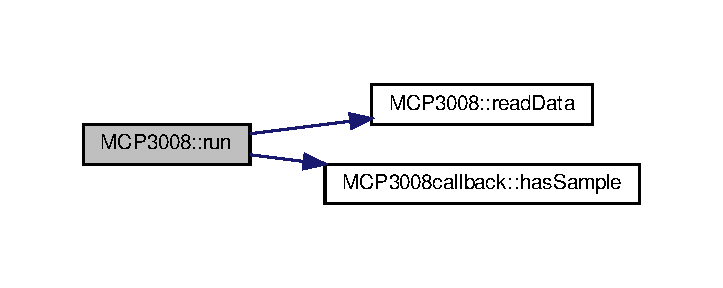
\includegraphics[width=347pt]{classMCP3008_a8e243711492e50dd4327050ffae8851d_cgraph}
\end{center}
\end{figure}
Here is the caller graph for this function\+:
\nopagebreak
\begin{figure}[H]
\begin{center}
\leavevmode
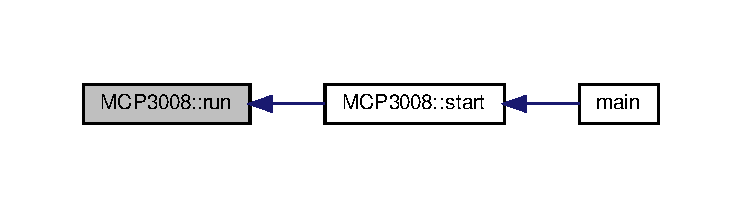
\includegraphics[width=350pt]{classMCP3008_a8e243711492e50dd4327050ffae8851d_icgraph}
\end{center}
\end{figure}
\mbox{\Hypertarget{classMCP3008_ad1893b9dd4dbbc2efbb57843871596fc}\label{classMCP3008_ad1893b9dd4dbbc2efbb57843871596fc}} 
\index{M\+C\+P3008@{M\+C\+P3008}!set\+\_\+channel@{set\+\_\+channel}}
\index{set\+\_\+channel@{set\+\_\+channel}!M\+C\+P3008@{M\+C\+P3008}}
\subsubsection{\texorpdfstring{set\+\_\+channel()}{set\_channel()}}
{\footnotesize\ttfamily void M\+C\+P3008\+::set\+\_\+channel (\begin{DoxyParamCaption}\item[{uint8\+\_\+t}]{channel }\end{DoxyParamCaption})}

function that allows to set channel of A\+DC from 0 to 7 Here is the caller graph for this function\+:
\nopagebreak
\begin{figure}[H]
\begin{center}
\leavevmode
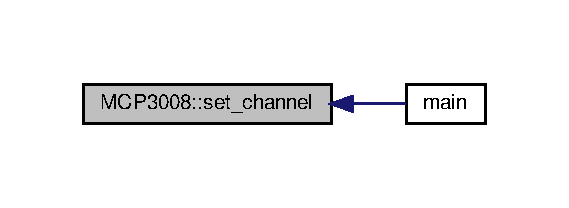
\includegraphics[width=273pt]{classMCP3008_ad1893b9dd4dbbc2efbb57843871596fc_icgraph}
\end{center}
\end{figure}
\mbox{\Hypertarget{classMCP3008_abe098bf3c4c2e6a803c53297d84e3c1c}\label{classMCP3008_abe098bf3c4c2e6a803c53297d84e3c1c}} 
\index{M\+C\+P3008@{M\+C\+P3008}!set\+Call\+Back@{set\+Call\+Back}}
\index{set\+Call\+Back@{set\+Call\+Back}!M\+C\+P3008@{M\+C\+P3008}}
\subsubsection{\texorpdfstring{set\+Call\+Back()}{setCallBack()}}
{\footnotesize\ttfamily void M\+C\+P3008\+::set\+Call\+Back (\begin{DoxyParamCaption}\item[{\hyperlink{classMCP3008callback}{M\+C\+P3008callback} $\ast$}]{cb }\end{DoxyParamCaption})}

function that allows to threads to set callbacks Here is the caller graph for this function\+:
\nopagebreak
\begin{figure}[H]
\begin{center}
\leavevmode
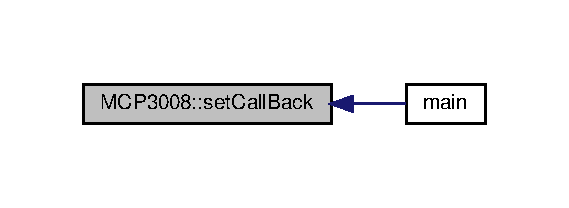
\includegraphics[width=273pt]{classMCP3008_abe098bf3c4c2e6a803c53297d84e3c1c_icgraph}
\end{center}
\end{figure}
\mbox{\Hypertarget{classMCP3008_a839bea8d430ee0852620c151c4467450}\label{classMCP3008_a839bea8d430ee0852620c151c4467450}} 
\index{M\+C\+P3008@{M\+C\+P3008}!start@{start}}
\index{start@{start}!M\+C\+P3008@{M\+C\+P3008}}
\subsubsection{\texorpdfstring{start()}{start()}}
{\footnotesize\ttfamily void M\+C\+P3008\+::start (\begin{DoxyParamCaption}{ }\end{DoxyParamCaption})}

Starts the data acquisition in the background and the callback is called with new samples Here is the call graph for this function\+:
\nopagebreak
\begin{figure}[H]
\begin{center}
\leavevmode
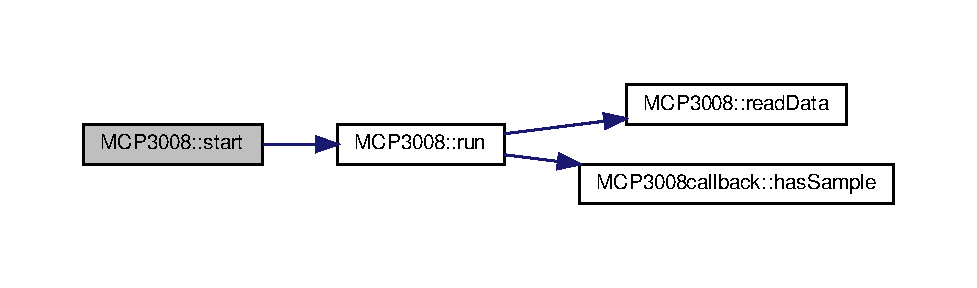
\includegraphics[width=350pt]{classMCP3008_a839bea8d430ee0852620c151c4467450_cgraph}
\end{center}
\end{figure}
Here is the caller graph for this function\+:
\nopagebreak
\begin{figure}[H]
\begin{center}
\leavevmode
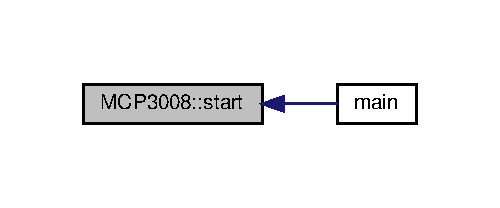
\includegraphics[width=240pt]{classMCP3008_a839bea8d430ee0852620c151c4467450_icgraph}
\end{center}
\end{figure}
\mbox{\Hypertarget{classMCP3008_add8fa4dafb68c227cd1ed269bd30603f}\label{classMCP3008_add8fa4dafb68c227cd1ed269bd30603f}} 
\index{M\+C\+P3008@{M\+C\+P3008}!stop@{stop}}
\index{stop@{stop}!M\+C\+P3008@{M\+C\+P3008}}
\subsubsection{\texorpdfstring{stop()}{stop()}}
{\footnotesize\ttfamily void M\+C\+P3008\+::stop (\begin{DoxyParamCaption}{ }\end{DoxyParamCaption})}

Stops the data acquisition Here is the caller graph for this function\+:
\nopagebreak
\begin{figure}[H]
\begin{center}
\leavevmode
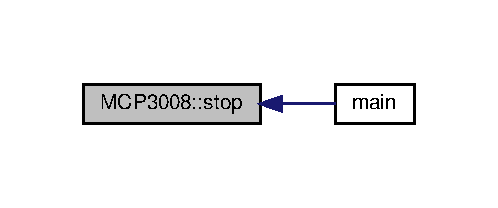
\includegraphics[width=239pt]{classMCP3008_add8fa4dafb68c227cd1ed269bd30603f_icgraph}
\end{center}
\end{figure}


\subsection{Field Documentation}
\mbox{\Hypertarget{classMCP3008_a9089ac2e245b158411670c802e6ea404}\label{classMCP3008_a9089ac2e245b158411670c802e6ea404}} 
\index{M\+C\+P3008@{M\+C\+P3008}!adc\+\_\+channel@{adc\+\_\+channel}}
\index{adc\+\_\+channel@{adc\+\_\+channel}!M\+C\+P3008@{M\+C\+P3008}}
\subsubsection{\texorpdfstring{adc\+\_\+channel}{adc\_channel}}
{\footnotesize\ttfamily uint8\+\_\+t M\+C\+P3008\+::adc\+\_\+channel\hspace{0.3cm}{\ttfamily [private]}}

\mbox{\Hypertarget{classMCP3008_ab1318bf3a8ac2bdf31b62451d29e1c90}\label{classMCP3008_ab1318bf3a8ac2bdf31b62451d29e1c90}} 
\index{M\+C\+P3008@{M\+C\+P3008}!adc\+Thread@{adc\+Thread}}
\index{adc\+Thread@{adc\+Thread}!M\+C\+P3008@{M\+C\+P3008}}
\subsubsection{\texorpdfstring{adc\+Thread}{adcThread}}
{\footnotesize\ttfamily std\+::thread$\ast$ M\+C\+P3008\+::adc\+Thread = N\+U\+LL\hspace{0.3cm}{\ttfamily [private]}}

\mbox{\Hypertarget{classMCP3008_a602724521657fd93241ba51c8dd83e74}\label{classMCP3008_a602724521657fd93241ba51c8dd83e74}} 
\index{M\+C\+P3008@{M\+C\+P3008}!mcp3008callback@{mcp3008callback}}
\index{mcp3008callback@{mcp3008callback}!M\+C\+P3008@{M\+C\+P3008}}
\subsubsection{\texorpdfstring{mcp3008callback}{mcp3008callback}}
{\footnotesize\ttfamily \hyperlink{classMCP3008callback}{M\+C\+P3008callback}$\ast$ M\+C\+P3008\+::mcp3008callback = N\+U\+LL\hspace{0.3cm}{\ttfamily [private]}}

\mbox{\Hypertarget{classMCP3008_a81354e1933a79bcb9f1d01c0e16566f0}\label{classMCP3008_a81354e1933a79bcb9f1d01c0e16566f0}} 
\index{M\+C\+P3008@{M\+C\+P3008}!running@{running}}
\index{running@{running}!M\+C\+P3008@{M\+C\+P3008}}
\subsubsection{\texorpdfstring{running}{running}}
{\footnotesize\ttfamily int M\+C\+P3008\+::running = 0\hspace{0.3cm}{\ttfamily [private]}}



The documentation for this class was generated from the following files\+:\begin{DoxyCompactItemize}
\item 
src/\hyperlink{MCP3008_8h}{M\+C\+P3008.\+h}\item 
src/\hyperlink{MCP3008_8cpp}{M\+C\+P3008.\+cpp}\end{DoxyCompactItemize}

\hypertarget{classMCP3008callback}{}\section{M\+C\+P3008callback Class Reference}
\label{classMCP3008callback}\index{M\+C\+P3008callback@{M\+C\+P3008callback}}


{\ttfamily \#include $<$M\+C\+P3008.\+h$>$}



Inheritance diagram for M\+C\+P3008callback\+:
\nopagebreak
\begin{figure}[H]
\begin{center}
\leavevmode
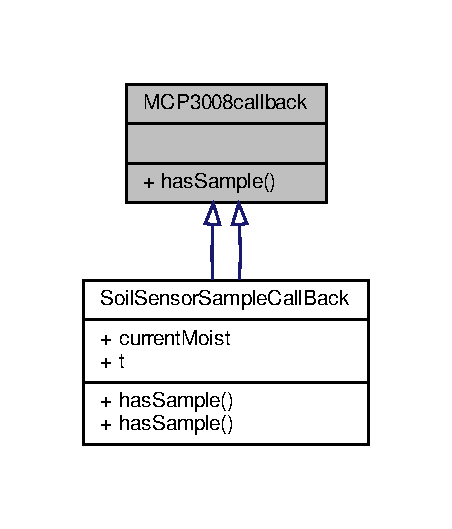
\includegraphics[width=217pt]{classMCP3008callback__inherit__graph}
\end{center}
\end{figure}


Collaboration diagram for M\+C\+P3008callback\+:
\nopagebreak
\begin{figure}[H]
\begin{center}
\leavevmode
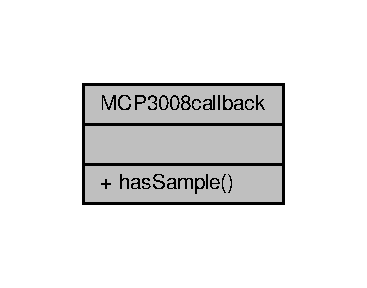
\includegraphics[width=176pt]{classMCP3008callback__coll__graph}
\end{center}
\end{figure}
\subsection*{Public Member Functions}
\begin{DoxyCompactItemize}
\item 
virtual void \hyperlink{classMCP3008callback_ad8c681193caaa955bf123666fc91e06a}{has\+Sample} (int sample)=0
\end{DoxyCompactItemize}


\subsection{Detailed Description}
Callback for new samples which needs to be implemented by the main program. The function has\+Sample needs to be overloaded in the main program. 

\subsection{Member Function Documentation}
\mbox{\Hypertarget{classMCP3008callback_ad8c681193caaa955bf123666fc91e06a}\label{classMCP3008callback_ad8c681193caaa955bf123666fc91e06a}} 
\index{M\+C\+P3008callback@{M\+C\+P3008callback}!has\+Sample@{has\+Sample}}
\index{has\+Sample@{has\+Sample}!M\+C\+P3008callback@{M\+C\+P3008callback}}
\subsubsection{\texorpdfstring{has\+Sample()}{hasSample()}}
{\footnotesize\ttfamily virtual void M\+C\+P3008callback\+::has\+Sample (\begin{DoxyParamCaption}\item[{int}]{sample }\end{DoxyParamCaption})\hspace{0.3cm}{\ttfamily [pure virtual]}}

Called after a sample has arrived. 

Implemented in \hyperlink{classSoilSensorSampleCallBack_a6bacdcc40b01f6a427f0f9ef2210fa76}{Soil\+Sensor\+Sample\+Call\+Back}, and \hyperlink{classSoilSensorSampleCallBack_a6bacdcc40b01f6a427f0f9ef2210fa76}{Soil\+Sensor\+Sample\+Call\+Back}.

Here is the caller graph for this function\+:
\nopagebreak
\begin{figure}[H]
\begin{center}
\leavevmode
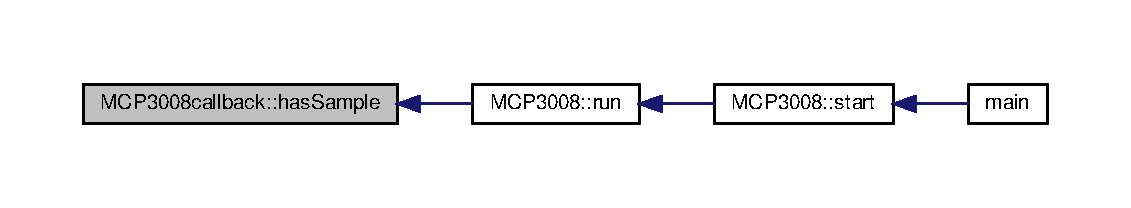
\includegraphics[width=350pt]{classMCP3008callback_ad8c681193caaa955bf123666fc91e06a_icgraph}
\end{center}
\end{figure}


The documentation for this class was generated from the following file\+:\begin{DoxyCompactItemize}
\item 
src/\hyperlink{MCP3008_8h}{M\+C\+P3008.\+h}\end{DoxyCompactItemize}

\hypertarget{classJSONCGIHandler_1_1POSTCallback}{}\section{J\+S\+O\+N\+C\+G\+I\+Handler\+:\+:P\+O\+S\+T\+Callback Class Reference}
\label{classJSONCGIHandler_1_1POSTCallback}\index{J\+S\+O\+N\+C\+G\+I\+Handler\+::\+P\+O\+S\+T\+Callback@{J\+S\+O\+N\+C\+G\+I\+Handler\+::\+P\+O\+S\+T\+Callback}}


{\ttfamily \#include $<$json\+\_\+fastcgi\+\_\+web\+\_\+api.\+h$>$}



Collaboration diagram for J\+S\+O\+N\+C\+G\+I\+Handler\+:\+:P\+O\+S\+T\+Callback\+:
\nopagebreak
\begin{figure}[H]
\begin{center}
\leavevmode
\includegraphics[width=247pt]{classJSONCGIHandler_1_1POSTCallback__coll__graph}
\end{center}
\end{figure}
\subsection*{Public Member Functions}
\begin{DoxyCompactItemize}
\item 
virtual void \hyperlink{classJSONCGIHandler_1_1POSTCallback_a6cddb384a3fd9242b323cea3d82a6bb7}{post\+String} (std\+::string post\+Arg)=0
\end{DoxyCompactItemize}


\subsection{Detailed Description}
Callback handler which needs to be implemented by the main program. 

\subsection{Member Function Documentation}
\mbox{\Hypertarget{classJSONCGIHandler_1_1POSTCallback_a6cddb384a3fd9242b323cea3d82a6bb7}\label{classJSONCGIHandler_1_1POSTCallback_a6cddb384a3fd9242b323cea3d82a6bb7}} 
\index{J\+S\+O\+N\+C\+G\+I\+Handler\+::\+P\+O\+S\+T\+Callback@{J\+S\+O\+N\+C\+G\+I\+Handler\+::\+P\+O\+S\+T\+Callback}!post\+String@{post\+String}}
\index{post\+String@{post\+String}!J\+S\+O\+N\+C\+G\+I\+Handler\+::\+P\+O\+S\+T\+Callback@{J\+S\+O\+N\+C\+G\+I\+Handler\+::\+P\+O\+S\+T\+Callback}}
\subsubsection{\texorpdfstring{post\+String()}{postString()}}
{\footnotesize\ttfamily virtual void J\+S\+O\+N\+C\+G\+I\+Handler\+::\+P\+O\+S\+T\+Callback\+::post\+String (\begin{DoxyParamCaption}\item[{std\+::string}]{post\+Arg }\end{DoxyParamCaption})\hspace{0.3cm}{\ttfamily [pure virtual]}}

Receives the P\+O\+ST data from the web browser. Use \hyperlink{classJSONCGIHandler_a0f208af3dd050ed182967fe9cca42d78}{post\+Decoder()} to decode the post\+Arg string. 
\begin{DoxyParams}{Parameters}
{\em post\+Arg} & P\+O\+ST data received from j\+Query \\
\hline
\end{DoxyParams}
Here is the caller graph for this function\+:
\nopagebreak
\begin{figure}[H]
\begin{center}
\leavevmode
\includegraphics[width=350pt]{classJSONCGIHandler_1_1POSTCallback_a6cddb384a3fd9242b323cea3d82a6bb7_icgraph}
\end{center}
\end{figure}


The documentation for this class was generated from the following file\+:\begin{DoxyCompactItemize}
\item 
src/\hyperlink{json__fastcgi__web__api_8h}{json\+\_\+fastcgi\+\_\+web\+\_\+api.\+h}\end{DoxyCompactItemize}

\hypertarget{classpump}{}\section{pump Class Reference}
\label{classpump}\index{pump@{pump}}


{\ttfamily \#include $<$pump.\+h$>$}



Collaboration diagram for pump\+:
\nopagebreak
\begin{figure}[H]
\begin{center}
\leavevmode
\includegraphics[width=157pt]{classpump__coll__graph}
\end{center}
\end{figure}
\subsection*{Public Member Functions}
\begin{DoxyCompactItemize}
\item 
\hyperlink{classpump_a57d3d6b37505970fc9524064fdc46b96}{pump} (int \hyperlink{classpump_a31d0a2af60c2193f5e5a6e4e51c56ec6}{relay})
\item 
\hyperlink{classpump_a17a634b5d8443578744bbd4c9eff9d87}{$\sim$pump} ()
\item 
void \hyperlink{classpump_a3c9536b9c3d2fdb7908b6cba845990d1}{set\+Pin} (int p)
\item 
void \hyperlink{classpump_a324936e9353f28b7633e838a9f1fff20}{start} ()
\item 
void \hyperlink{classpump_add87c3bee2a6faba0404e9ce115d0d17}{stop} ()
\end{DoxyCompactItemize}
\subsection*{Private Member Functions}
\begin{DoxyCompactItemize}
\item 
void \hyperlink{classpump_af6264b2a6b6e66ed1027565a44561647}{onoff} ()
\end{DoxyCompactItemize}
\subsection*{Static Private Member Functions}
\begin{DoxyCompactItemize}
\item 
static void \hyperlink{classpump_a058e2690d8022501b5dfdc4ca646cb7c}{run} (\hyperlink{classpump}{pump} $\ast$p)
\end{DoxyCompactItemize}
\subsection*{Private Attributes}
\begin{DoxyCompactItemize}
\item 
std\+::string \hyperlink{classpump_ad96353945f20f718e8eba930fa8405ba}{state}
\item 
int \hyperlink{classpump_a31d0a2af60c2193f5e5a6e4e51c56ec6}{relay}
\item 
int \hyperlink{classpump_ad797d26b29fe1ebf7ad6f6590fb2c674}{running} = 0
\item 
std\+::thread $\ast$ \hyperlink{classpump_a52d8740c4bc37939ead02e93a6dfdb68}{pump\+Thread} = N\+U\+LL
\end{DoxyCompactItemize}


\subsection{Constructor \& Destructor Documentation}
\mbox{\Hypertarget{classpump_a57d3d6b37505970fc9524064fdc46b96}\label{classpump_a57d3d6b37505970fc9524064fdc46b96}} 
\index{pump@{pump}!pump@{pump}}
\index{pump@{pump}!pump@{pump}}
\subsubsection{\texorpdfstring{pump()}{pump()}}
{\footnotesize\ttfamily pump\+::pump (\begin{DoxyParamCaption}\item[{int}]{relay }\end{DoxyParamCaption})}

clas constructor Here is the call graph for this function\+:
\nopagebreak
\begin{figure}[H]
\begin{center}
\leavevmode
\includegraphics[width=261pt]{classpump_a57d3d6b37505970fc9524064fdc46b96_cgraph}
\end{center}
\end{figure}
\mbox{\Hypertarget{classpump_a17a634b5d8443578744bbd4c9eff9d87}\label{classpump_a17a634b5d8443578744bbd4c9eff9d87}} 
\index{pump@{pump}!````~pump@{$\sim$pump}}
\index{````~pump@{$\sim$pump}!pump@{pump}}
\subsubsection{\texorpdfstring{$\sim$pump()}{~pump()}}
{\footnotesize\ttfamily pump\+::$\sim$pump (\begin{DoxyParamCaption}{ }\end{DoxyParamCaption})\hspace{0.3cm}{\ttfamily [inline]}}

clas constructor Here is the call graph for this function\+:
\nopagebreak
\begin{figure}[H]
\begin{center}
\leavevmode
\includegraphics[width=350pt]{classpump_a17a634b5d8443578744bbd4c9eff9d87_cgraph}
\end{center}
\end{figure}


\subsection{Member Function Documentation}
\mbox{\Hypertarget{classpump_af6264b2a6b6e66ed1027565a44561647}\label{classpump_af6264b2a6b6e66ed1027565a44561647}} 
\index{pump@{pump}!onoff@{onoff}}
\index{onoff@{onoff}!pump@{pump}}
\subsubsection{\texorpdfstring{onoff()}{onoff()}}
{\footnotesize\ttfamily void pump\+::onoff (\begin{DoxyParamCaption}{ }\end{DoxyParamCaption})\hspace{0.3cm}{\ttfamily [private]}}

Here is the caller graph for this function\+:
\nopagebreak
\begin{figure}[H]
\begin{center}
\leavevmode
\includegraphics[width=350pt]{classpump_af6264b2a6b6e66ed1027565a44561647_icgraph}
\end{center}
\end{figure}
\mbox{\Hypertarget{classpump_a058e2690d8022501b5dfdc4ca646cb7c}\label{classpump_a058e2690d8022501b5dfdc4ca646cb7c}} 
\index{pump@{pump}!run@{run}}
\index{run@{run}!pump@{pump}}
\subsubsection{\texorpdfstring{run()}{run()}}
{\footnotesize\ttfamily void pump\+::run (\begin{DoxyParamCaption}\item[{\hyperlink{classpump}{pump} $\ast$}]{p }\end{DoxyParamCaption})\hspace{0.3cm}{\ttfamily [static]}, {\ttfamily [private]}}

Here is the call graph for this function\+:
\nopagebreak
\begin{figure}[H]
\begin{center}
\leavevmode
\includegraphics[width=244pt]{classpump_a058e2690d8022501b5dfdc4ca646cb7c_cgraph}
\end{center}
\end{figure}
Here is the caller graph for this function\+:
\nopagebreak
\begin{figure}[H]
\begin{center}
\leavevmode
\includegraphics[width=350pt]{classpump_a058e2690d8022501b5dfdc4ca646cb7c_icgraph}
\end{center}
\end{figure}
\mbox{\Hypertarget{classpump_a3c9536b9c3d2fdb7908b6cba845990d1}\label{classpump_a3c9536b9c3d2fdb7908b6cba845990d1}} 
\index{pump@{pump}!set\+Pin@{set\+Pin}}
\index{set\+Pin@{set\+Pin}!pump@{pump}}
\subsubsection{\texorpdfstring{set\+Pin()}{setPin()}}
{\footnotesize\ttfamily void pump\+::set\+Pin (\begin{DoxyParamCaption}\item[{int}]{p }\end{DoxyParamCaption})}

function that allows to set the G\+P\+IO pin Here is the caller graph for this function\+:
\nopagebreak
\begin{figure}[H]
\begin{center}
\leavevmode
\includegraphics[width=267pt]{classpump_a3c9536b9c3d2fdb7908b6cba845990d1_icgraph}
\end{center}
\end{figure}
\mbox{\Hypertarget{classpump_a324936e9353f28b7633e838a9f1fff20}\label{classpump_a324936e9353f28b7633e838a9f1fff20}} 
\index{pump@{pump}!start@{start}}
\index{start@{start}!pump@{pump}}
\subsubsection{\texorpdfstring{start()}{start()}}
{\footnotesize\ttfamily void pump\+::start (\begin{DoxyParamCaption}{ }\end{DoxyParamCaption})}

starts the pump logic Here is the call graph for this function\+:
\nopagebreak
\begin{figure}[H]
\begin{center}
\leavevmode
\includegraphics[width=346pt]{classpump_a324936e9353f28b7633e838a9f1fff20_cgraph}
\end{center}
\end{figure}
Here is the caller graph for this function\+:
\nopagebreak
\begin{figure}[H]
\begin{center}
\leavevmode
\includegraphics[width=259pt]{classpump_a324936e9353f28b7633e838a9f1fff20_icgraph}
\end{center}
\end{figure}
\mbox{\Hypertarget{classpump_add87c3bee2a6faba0404e9ce115d0d17}\label{classpump_add87c3bee2a6faba0404e9ce115d0d17}} 
\index{pump@{pump}!stop@{stop}}
\index{stop@{stop}!pump@{pump}}
\subsubsection{\texorpdfstring{stop()}{stop()}}
{\footnotesize\ttfamily void pump\+::stop (\begin{DoxyParamCaption}{ }\end{DoxyParamCaption})}

stops the pump logic Here is the caller graph for this function\+:
\nopagebreak
\begin{figure}[H]
\begin{center}
\leavevmode
\includegraphics[width=258pt]{classpump_add87c3bee2a6faba0404e9ce115d0d17_icgraph}
\end{center}
\end{figure}


\subsection{Field Documentation}
\mbox{\Hypertarget{classpump_a52d8740c4bc37939ead02e93a6dfdb68}\label{classpump_a52d8740c4bc37939ead02e93a6dfdb68}} 
\index{pump@{pump}!pump\+Thread@{pump\+Thread}}
\index{pump\+Thread@{pump\+Thread}!pump@{pump}}
\subsubsection{\texorpdfstring{pump\+Thread}{pumpThread}}
{\footnotesize\ttfamily std\+::thread$\ast$ pump\+::pump\+Thread = N\+U\+LL\hspace{0.3cm}{\ttfamily [private]}}

\mbox{\Hypertarget{classpump_a31d0a2af60c2193f5e5a6e4e51c56ec6}\label{classpump_a31d0a2af60c2193f5e5a6e4e51c56ec6}} 
\index{pump@{pump}!relay@{relay}}
\index{relay@{relay}!pump@{pump}}
\subsubsection{\texorpdfstring{relay}{relay}}
{\footnotesize\ttfamily int pump\+::relay\hspace{0.3cm}{\ttfamily [private]}}

\mbox{\Hypertarget{classpump_ad797d26b29fe1ebf7ad6f6590fb2c674}\label{classpump_ad797d26b29fe1ebf7ad6f6590fb2c674}} 
\index{pump@{pump}!running@{running}}
\index{running@{running}!pump@{pump}}
\subsubsection{\texorpdfstring{running}{running}}
{\footnotesize\ttfamily int pump\+::running = 0\hspace{0.3cm}{\ttfamily [private]}}

\mbox{\Hypertarget{classpump_ad96353945f20f718e8eba930fa8405ba}\label{classpump_ad96353945f20f718e8eba930fa8405ba}} 
\index{pump@{pump}!state@{state}}
\index{state@{state}!pump@{pump}}
\subsubsection{\texorpdfstring{state}{state}}
{\footnotesize\ttfamily std\+::string pump\+::state\hspace{0.3cm}{\ttfamily [private]}}



The documentation for this class was generated from the following files\+:\begin{DoxyCompactItemize}
\item 
src/\hyperlink{pump_8h}{pump.\+h}\item 
src/\hyperlink{pump_8cpp}{pump.\+cpp}\end{DoxyCompactItemize}

\hypertarget{classSoilSensorSampleCallBack}{}\section{Soil\+Sensor\+Sample\+Call\+Back Class Reference}
\label{classSoilSensorSampleCallBack}\index{Soil\+Sensor\+Sample\+Call\+Back@{Soil\+Sensor\+Sample\+Call\+Back}}


Inheritance diagram for Soil\+Sensor\+Sample\+Call\+Back\+:
\nopagebreak
\begin{figure}[H]
\begin{center}
\leavevmode
\includegraphics[width=217pt]{classSoilSensorSampleCallBack__inherit__graph}
\end{center}
\end{figure}


Collaboration diagram for Soil\+Sensor\+Sample\+Call\+Back\+:
\nopagebreak
\begin{figure}[H]
\begin{center}
\leavevmode
\includegraphics[width=217pt]{classSoilSensorSampleCallBack__coll__graph}
\end{center}
\end{figure}
\subsection*{Public Member Functions}
\begin{DoxyCompactItemize}
\item 
virtual void \hyperlink{classSoilSensorSampleCallBack_a6bacdcc40b01f6a427f0f9ef2210fa76}{has\+Sample} (int s)
\item 
virtual void \hyperlink{classSoilSensorSampleCallBack_a6bacdcc40b01f6a427f0f9ef2210fa76}{has\+Sample} (int s)
\end{DoxyCompactItemize}
\subsection*{Data Fields}
\begin{DoxyCompactItemize}
\item 
int \hyperlink{classSoilSensorSampleCallBack_a0f82c27a02ffa86512ff83f92a4a6e93}{current\+Moist}
\item 
long \hyperlink{classSoilSensorSampleCallBack_a27c6796e420396b73a1c05019a613c31}{t}
\end{DoxyCompactItemize}


\subsection{Member Function Documentation}
\mbox{\Hypertarget{classSoilSensorSampleCallBack_a6bacdcc40b01f6a427f0f9ef2210fa76}\label{classSoilSensorSampleCallBack_a6bacdcc40b01f6a427f0f9ef2210fa76}} 
\index{Soil\+Sensor\+Sample\+Call\+Back@{Soil\+Sensor\+Sample\+Call\+Back}!has\+Sample@{has\+Sample}}
\index{has\+Sample@{has\+Sample}!Soil\+Sensor\+Sample\+Call\+Back@{Soil\+Sensor\+Sample\+Call\+Back}}
\subsubsection{\texorpdfstring{has\+Sample()}{hasSample()}\hspace{0.1cm}{\footnotesize\ttfamily [1/2]}}
{\footnotesize\ttfamily virtual void Soil\+Sensor\+Sample\+Call\+Back\+::has\+Sample (\begin{DoxyParamCaption}\item[{int}]{sample }\end{DoxyParamCaption})\hspace{0.3cm}{\ttfamily [inline]}, {\ttfamily [virtual]}}

Called after a sample has arrived. 

Implements \hyperlink{classMCP3008callback_ad8c681193caaa955bf123666fc91e06a}{M\+C\+P3008callback}.

\mbox{\Hypertarget{classSoilSensorSampleCallBack_a6bacdcc40b01f6a427f0f9ef2210fa76}\label{classSoilSensorSampleCallBack_a6bacdcc40b01f6a427f0f9ef2210fa76}} 
\index{Soil\+Sensor\+Sample\+Call\+Back@{Soil\+Sensor\+Sample\+Call\+Back}!has\+Sample@{has\+Sample}}
\index{has\+Sample@{has\+Sample}!Soil\+Sensor\+Sample\+Call\+Back@{Soil\+Sensor\+Sample\+Call\+Back}}
\subsubsection{\texorpdfstring{has\+Sample()}{hasSample()}\hspace{0.1cm}{\footnotesize\ttfamily [2/2]}}
{\footnotesize\ttfamily virtual void Soil\+Sensor\+Sample\+Call\+Back\+::has\+Sample (\begin{DoxyParamCaption}\item[{int}]{sample }\end{DoxyParamCaption})\hspace{0.3cm}{\ttfamily [inline]}, {\ttfamily [virtual]}}

Called after a sample has arrived. 

Implements \hyperlink{classMCP3008callback_ad8c681193caaa955bf123666fc91e06a}{M\+C\+P3008callback}.



\subsection{Field Documentation}
\mbox{\Hypertarget{classSoilSensorSampleCallBack_a0f82c27a02ffa86512ff83f92a4a6e93}\label{classSoilSensorSampleCallBack_a0f82c27a02ffa86512ff83f92a4a6e93}} 
\index{Soil\+Sensor\+Sample\+Call\+Back@{Soil\+Sensor\+Sample\+Call\+Back}!current\+Moist@{current\+Moist}}
\index{current\+Moist@{current\+Moist}!Soil\+Sensor\+Sample\+Call\+Back@{Soil\+Sensor\+Sample\+Call\+Back}}
\subsubsection{\texorpdfstring{current\+Moist}{currentMoist}}
{\footnotesize\ttfamily int Soil\+Sensor\+Sample\+Call\+Back\+::current\+Moist}

\mbox{\Hypertarget{classSoilSensorSampleCallBack_a27c6796e420396b73a1c05019a613c31}\label{classSoilSensorSampleCallBack_a27c6796e420396b73a1c05019a613c31}} 
\index{Soil\+Sensor\+Sample\+Call\+Back@{Soil\+Sensor\+Sample\+Call\+Back}!t@{t}}
\index{t@{t}!Soil\+Sensor\+Sample\+Call\+Back@{Soil\+Sensor\+Sample\+Call\+Back}}
\subsubsection{\texorpdfstring{t}{t}}
{\footnotesize\ttfamily long Soil\+Sensor\+Sample\+Call\+Back\+::t}



The documentation for this class was generated from the following files\+:\begin{DoxyCompactItemize}
\item 
src/\hyperlink{demo_8cpp}{demo.\+cpp}\item 
src/\hyperlink{soil__callback_8cpp}{soil\+\_\+callback.\+cpp}\end{DoxyCompactItemize}

\hypertarget{classUltrasonic}{}\section{Ultrasonic Class Reference}
\label{classUltrasonic}\index{Ultrasonic@{Ultrasonic}}


{\ttfamily \#include $<$ultrasonic.\+h$>$}



Collaboration diagram for Ultrasonic\+:
\nopagebreak
\begin{figure}[H]
\begin{center}
\leavevmode
\includegraphics[width=191pt]{classUltrasonic__coll__graph}
\end{center}
\end{figure}
\subsection*{Public Member Functions}
\begin{DoxyCompactItemize}
\item 
\hyperlink{classUltrasonic_a306b1ccdce9cc1bfa3ef4a51502e7d44}{Ultrasonic} (int \hyperlink{classUltrasonic_a2979ecabfbda7cae5394eef20c862d99}{echo}, int \hyperlink{classUltrasonic_a90f3f5b30f09038811bcc5231efdc619}{trig})
\item 
\hyperlink{classUltrasonic_ab5066b2bfeac723140c18b9f8340abad}{$\sim$\+Ultrasonic} ()
\item 
void \hyperlink{classUltrasonic_aa0ede289109954e5b3c713bbebe8c8e1}{start} ()
\item 
void \hyperlink{classUltrasonic_ae5d433dfce8572b5cc1d75a909ae2c1c}{stop} ()
\item 
void \hyperlink{classUltrasonic_a0b9d6fed8f4d6a207a91f19763ba70fe}{set\+Call\+Back} (\hyperlink{classUltrasonicCallback}{Ultrasonic\+Callback} $\ast$cb)
\end{DoxyCompactItemize}
\subsection*{Private Member Functions}
\begin{DoxyCompactItemize}
\item 
void \hyperlink{classUltrasonic_a5ceb2f35156c7e6b6c22538b090b1923}{set\+Pin} (int e, int t)
\item 
int \hyperlink{classUltrasonic_a7af95864d8b2b58d56e661e0fcb4ca8b}{get\+Distance\+CM} ()
\end{DoxyCompactItemize}
\subsection*{Static Private Member Functions}
\begin{DoxyCompactItemize}
\item 
static void \hyperlink{classUltrasonic_ac1df91b01624260ce4c19126e3aa0160}{run} (\hyperlink{classUltrasonic}{Ultrasonic} $\ast$ultrasonic)
\end{DoxyCompactItemize}
\subsection*{Private Attributes}
\begin{DoxyCompactItemize}
\item 
\hyperlink{classUltrasonicCallback}{Ultrasonic\+Callback} $\ast$ \hyperlink{classUltrasonic_a00cb643880cff1ac6b3b429e92c5bba9}{ultrasonic\+Cb} = N\+U\+LL
\item 
int \hyperlink{classUltrasonic_a2979ecabfbda7cae5394eef20c862d99}{echo}
\item 
int \hyperlink{classUltrasonic_a90f3f5b30f09038811bcc5231efdc619}{trig}
\item 
std\+::thread $\ast$ \hyperlink{classUltrasonic_a830f5b7f4e3de362e1b90eb5d6f3844b}{ultra\+Thread} = N\+U\+LL
\item 
int \hyperlink{classUltrasonic_a18088bcacb3c6080c08c2ea105313f65}{running} = 0
\end{DoxyCompactItemize}


\subsection{Constructor \& Destructor Documentation}
\mbox{\Hypertarget{classUltrasonic_a306b1ccdce9cc1bfa3ef4a51502e7d44}\label{classUltrasonic_a306b1ccdce9cc1bfa3ef4a51502e7d44}} 
\index{Ultrasonic@{Ultrasonic}!Ultrasonic@{Ultrasonic}}
\index{Ultrasonic@{Ultrasonic}!Ultrasonic@{Ultrasonic}}
\subsubsection{\texorpdfstring{Ultrasonic()}{Ultrasonic()}}
{\footnotesize\ttfamily Ultrasonic\+::\+Ultrasonic (\begin{DoxyParamCaption}\item[{int}]{echo,  }\item[{int}]{trig }\end{DoxyParamCaption})}

Here is the call graph for this function\+:
\nopagebreak
\begin{figure}[H]
\begin{center}
\leavevmode
\includegraphics[width=322pt]{classUltrasonic_a306b1ccdce9cc1bfa3ef4a51502e7d44_cgraph}
\end{center}
\end{figure}
\mbox{\Hypertarget{classUltrasonic_ab5066b2bfeac723140c18b9f8340abad}\label{classUltrasonic_ab5066b2bfeac723140c18b9f8340abad}} 
\index{Ultrasonic@{Ultrasonic}!````~Ultrasonic@{$\sim$\+Ultrasonic}}
\index{````~Ultrasonic@{$\sim$\+Ultrasonic}!Ultrasonic@{Ultrasonic}}
\subsubsection{\texorpdfstring{$\sim$\+Ultrasonic()}{~Ultrasonic()}}
{\footnotesize\ttfamily Ultrasonic\+::$\sim$\+Ultrasonic (\begin{DoxyParamCaption}{ }\end{DoxyParamCaption})\hspace{0.3cm}{\ttfamily [inline]}}



\subsection{Member Function Documentation}
\mbox{\Hypertarget{classUltrasonic_a7af95864d8b2b58d56e661e0fcb4ca8b}\label{classUltrasonic_a7af95864d8b2b58d56e661e0fcb4ca8b}} 
\index{Ultrasonic@{Ultrasonic}!get\+Distance\+CM@{get\+Distance\+CM}}
\index{get\+Distance\+CM@{get\+Distance\+CM}!Ultrasonic@{Ultrasonic}}
\subsubsection{\texorpdfstring{get\+Distance\+C\+M()}{getDistanceCM()}}
{\footnotesize\ttfamily int Ultrasonic\+::get\+Distance\+CM (\begin{DoxyParamCaption}{ }\end{DoxyParamCaption})\hspace{0.3cm}{\ttfamily [private]}}

Here is the caller graph for this function\+:
\nopagebreak
\begin{figure}[H]
\begin{center}
\leavevmode
\includegraphics[width=350pt]{classUltrasonic_a7af95864d8b2b58d56e661e0fcb4ca8b_icgraph}
\end{center}
\end{figure}
\mbox{\Hypertarget{classUltrasonic_ac1df91b01624260ce4c19126e3aa0160}\label{classUltrasonic_ac1df91b01624260ce4c19126e3aa0160}} 
\index{Ultrasonic@{Ultrasonic}!run@{run}}
\index{run@{run}!Ultrasonic@{Ultrasonic}}
\subsubsection{\texorpdfstring{run()}{run()}}
{\footnotesize\ttfamily void Ultrasonic\+::run (\begin{DoxyParamCaption}\item[{\hyperlink{classUltrasonic}{Ultrasonic} $\ast$}]{ultrasonic }\end{DoxyParamCaption})\hspace{0.3cm}{\ttfamily [static]}, {\ttfamily [private]}}

Here is the call graph for this function\+:
\nopagebreak
\begin{figure}[H]
\begin{center}
\leavevmode
\includegraphics[width=331pt]{classUltrasonic_ac1df91b01624260ce4c19126e3aa0160_cgraph}
\end{center}
\end{figure}
Here is the caller graph for this function\+:
\nopagebreak
\begin{figure}[H]
\begin{center}
\leavevmode
\includegraphics[width=350pt]{classUltrasonic_ac1df91b01624260ce4c19126e3aa0160_icgraph}
\end{center}
\end{figure}
\mbox{\Hypertarget{classUltrasonic_a0b9d6fed8f4d6a207a91f19763ba70fe}\label{classUltrasonic_a0b9d6fed8f4d6a207a91f19763ba70fe}} 
\index{Ultrasonic@{Ultrasonic}!set\+Call\+Back@{set\+Call\+Back}}
\index{set\+Call\+Back@{set\+Call\+Back}!Ultrasonic@{Ultrasonic}}
\subsubsection{\texorpdfstring{set\+Call\+Back()}{setCallBack()}}
{\footnotesize\ttfamily void Ultrasonic\+::set\+Call\+Back (\begin{DoxyParamCaption}\item[{\hyperlink{classUltrasonicCallback}{Ultrasonic\+Callback} $\ast$}]{cb }\end{DoxyParamCaption})}

Here is the caller graph for this function\+:
\nopagebreak
\begin{figure}[H]
\begin{center}
\leavevmode
\includegraphics[width=274pt]{classUltrasonic_a0b9d6fed8f4d6a207a91f19763ba70fe_icgraph}
\end{center}
\end{figure}
\mbox{\Hypertarget{classUltrasonic_a5ceb2f35156c7e6b6c22538b090b1923}\label{classUltrasonic_a5ceb2f35156c7e6b6c22538b090b1923}} 
\index{Ultrasonic@{Ultrasonic}!set\+Pin@{set\+Pin}}
\index{set\+Pin@{set\+Pin}!Ultrasonic@{Ultrasonic}}
\subsubsection{\texorpdfstring{set\+Pin()}{setPin()}}
{\footnotesize\ttfamily void Ultrasonic\+::set\+Pin (\begin{DoxyParamCaption}\item[{int}]{e,  }\item[{int}]{t }\end{DoxyParamCaption})\hspace{0.3cm}{\ttfamily [private]}}

Here is the caller graph for this function\+:
\nopagebreak
\begin{figure}[H]
\begin{center}
\leavevmode
\includegraphics[width=322pt]{classUltrasonic_a5ceb2f35156c7e6b6c22538b090b1923_icgraph}
\end{center}
\end{figure}
\mbox{\Hypertarget{classUltrasonic_aa0ede289109954e5b3c713bbebe8c8e1}\label{classUltrasonic_aa0ede289109954e5b3c713bbebe8c8e1}} 
\index{Ultrasonic@{Ultrasonic}!start@{start}}
\index{start@{start}!Ultrasonic@{Ultrasonic}}
\subsubsection{\texorpdfstring{start()}{start()}}
{\footnotesize\ttfamily void Ultrasonic\+::start (\begin{DoxyParamCaption}{ }\end{DoxyParamCaption})}

Here is the call graph for this function\+:
\nopagebreak
\begin{figure}[H]
\begin{center}
\leavevmode
\includegraphics[width=350pt]{classUltrasonic_aa0ede289109954e5b3c713bbebe8c8e1_cgraph}
\end{center}
\end{figure}
Here is the caller graph for this function\+:
\nopagebreak
\begin{figure}[H]
\begin{center}
\leavevmode
\includegraphics[width=240pt]{classUltrasonic_aa0ede289109954e5b3c713bbebe8c8e1_icgraph}
\end{center}
\end{figure}
\mbox{\Hypertarget{classUltrasonic_ae5d433dfce8572b5cc1d75a909ae2c1c}\label{classUltrasonic_ae5d433dfce8572b5cc1d75a909ae2c1c}} 
\index{Ultrasonic@{Ultrasonic}!stop@{stop}}
\index{stop@{stop}!Ultrasonic@{Ultrasonic}}
\subsubsection{\texorpdfstring{stop()}{stop()}}
{\footnotesize\ttfamily void Ultrasonic\+::stop (\begin{DoxyParamCaption}{ }\end{DoxyParamCaption})}

Here is the caller graph for this function\+:
\nopagebreak
\begin{figure}[H]
\begin{center}
\leavevmode
\includegraphics[width=240pt]{classUltrasonic_ae5d433dfce8572b5cc1d75a909ae2c1c_icgraph}
\end{center}
\end{figure}


\subsection{Field Documentation}
\mbox{\Hypertarget{classUltrasonic_a2979ecabfbda7cae5394eef20c862d99}\label{classUltrasonic_a2979ecabfbda7cae5394eef20c862d99}} 
\index{Ultrasonic@{Ultrasonic}!echo@{echo}}
\index{echo@{echo}!Ultrasonic@{Ultrasonic}}
\subsubsection{\texorpdfstring{echo}{echo}}
{\footnotesize\ttfamily int Ultrasonic\+::echo\hspace{0.3cm}{\ttfamily [private]}}

\mbox{\Hypertarget{classUltrasonic_a18088bcacb3c6080c08c2ea105313f65}\label{classUltrasonic_a18088bcacb3c6080c08c2ea105313f65}} 
\index{Ultrasonic@{Ultrasonic}!running@{running}}
\index{running@{running}!Ultrasonic@{Ultrasonic}}
\subsubsection{\texorpdfstring{running}{running}}
{\footnotesize\ttfamily int Ultrasonic\+::running = 0\hspace{0.3cm}{\ttfamily [private]}}

\mbox{\Hypertarget{classUltrasonic_a90f3f5b30f09038811bcc5231efdc619}\label{classUltrasonic_a90f3f5b30f09038811bcc5231efdc619}} 
\index{Ultrasonic@{Ultrasonic}!trig@{trig}}
\index{trig@{trig}!Ultrasonic@{Ultrasonic}}
\subsubsection{\texorpdfstring{trig}{trig}}
{\footnotesize\ttfamily int Ultrasonic\+::trig\hspace{0.3cm}{\ttfamily [private]}}

\mbox{\Hypertarget{classUltrasonic_a00cb643880cff1ac6b3b429e92c5bba9}\label{classUltrasonic_a00cb643880cff1ac6b3b429e92c5bba9}} 
\index{Ultrasonic@{Ultrasonic}!ultrasonic\+Cb@{ultrasonic\+Cb}}
\index{ultrasonic\+Cb@{ultrasonic\+Cb}!Ultrasonic@{Ultrasonic}}
\subsubsection{\texorpdfstring{ultrasonic\+Cb}{ultrasonicCb}}
{\footnotesize\ttfamily \hyperlink{classUltrasonicCallback}{Ultrasonic\+Callback}$\ast$ Ultrasonic\+::ultrasonic\+Cb = N\+U\+LL\hspace{0.3cm}{\ttfamily [private]}}

\mbox{\Hypertarget{classUltrasonic_a830f5b7f4e3de362e1b90eb5d6f3844b}\label{classUltrasonic_a830f5b7f4e3de362e1b90eb5d6f3844b}} 
\index{Ultrasonic@{Ultrasonic}!ultra\+Thread@{ultra\+Thread}}
\index{ultra\+Thread@{ultra\+Thread}!Ultrasonic@{Ultrasonic}}
\subsubsection{\texorpdfstring{ultra\+Thread}{ultraThread}}
{\footnotesize\ttfamily std\+::thread$\ast$ Ultrasonic\+::ultra\+Thread = N\+U\+LL\hspace{0.3cm}{\ttfamily [private]}}



The documentation for this class was generated from the following files\+:\begin{DoxyCompactItemize}
\item 
src/\hyperlink{ultrasonic_8h}{ultrasonic.\+h}\item 
src/\hyperlink{ultrasonic_8cpp}{ultrasonic.\+cpp}\end{DoxyCompactItemize}

\hypertarget{classUltrasonicCallback}{}\section{Ultrasonic\+Callback Class Reference}
\label{classUltrasonicCallback}\index{Ultrasonic\+Callback@{Ultrasonic\+Callback}}


{\ttfamily \#include $<$ultrasonic.\+h$>$}



Inheritance diagram for Ultrasonic\+Callback\+:
\nopagebreak
\begin{figure}[H]
\begin{center}
\leavevmode
\includegraphics[width=244pt]{classUltrasonicCallback__inherit__graph}
\end{center}
\end{figure}


Collaboration diagram for Ultrasonic\+Callback\+:
\nopagebreak
\begin{figure}[H]
\begin{center}
\leavevmode
\includegraphics[width=179pt]{classUltrasonicCallback__coll__graph}
\end{center}
\end{figure}
\subsection*{Public Member Functions}
\begin{DoxyCompactItemize}
\item 
virtual void \hyperlink{classUltrasonicCallback_aded93e2bea7669f1f225f8b35a085052}{has\+Sample} (int d)=0
\end{DoxyCompactItemize}


\subsection{Member Function Documentation}
\mbox{\Hypertarget{classUltrasonicCallback_aded93e2bea7669f1f225f8b35a085052}\label{classUltrasonicCallback_aded93e2bea7669f1f225f8b35a085052}} 
\index{Ultrasonic\+Callback@{Ultrasonic\+Callback}!has\+Sample@{has\+Sample}}
\index{has\+Sample@{has\+Sample}!Ultrasonic\+Callback@{Ultrasonic\+Callback}}
\subsubsection{\texorpdfstring{has\+Sample()}{hasSample()}}
{\footnotesize\ttfamily virtual void Ultrasonic\+Callback\+::has\+Sample (\begin{DoxyParamCaption}\item[{int}]{d }\end{DoxyParamCaption})\hspace{0.3cm}{\ttfamily [pure virtual]}}



Implemented in \hyperlink{classUltraSonicSensorSampleCallback_abe420043f2ea2123654d55d06d9315ac}{Ultra\+Sonic\+Sensor\+Sample\+Callback}, and \hyperlink{classUltraSonicSensorSampleCallback_abe420043f2ea2123654d55d06d9315ac}{Ultra\+Sonic\+Sensor\+Sample\+Callback}.

Here is the caller graph for this function\+:
\nopagebreak
\begin{figure}[H]
\begin{center}
\leavevmode
\includegraphics[width=350pt]{classUltrasonicCallback_aded93e2bea7669f1f225f8b35a085052_icgraph}
\end{center}
\end{figure}


The documentation for this class was generated from the following file\+:\begin{DoxyCompactItemize}
\item 
src/\hyperlink{ultrasonic_8h}{ultrasonic.\+h}\end{DoxyCompactItemize}

\hypertarget{classUltraSonicSensorSampleCallback}{}\section{Ultra\+Sonic\+Sensor\+Sample\+Callback Class Reference}
\label{classUltraSonicSensorSampleCallback}\index{Ultra\+Sonic\+Sensor\+Sample\+Callback@{Ultra\+Sonic\+Sensor\+Sample\+Callback}}


Inheritance diagram for Ultra\+Sonic\+Sensor\+Sample\+Callback\+:
\nopagebreak
\begin{figure}[H]
\begin{center}
\leavevmode
\includegraphics[width=244pt]{classUltraSonicSensorSampleCallback__inherit__graph}
\end{center}
\end{figure}


Collaboration diagram for Ultra\+Sonic\+Sensor\+Sample\+Callback\+:
\nopagebreak
\begin{figure}[H]
\begin{center}
\leavevmode
\includegraphics[width=244pt]{classUltraSonicSensorSampleCallback__coll__graph}
\end{center}
\end{figure}
\subsection*{Public Member Functions}
\begin{DoxyCompactItemize}
\item 
virtual void \hyperlink{classUltraSonicSensorSampleCallback_abe420043f2ea2123654d55d06d9315ac}{has\+Sample} (int d)
\item 
virtual void \hyperlink{classUltraSonicSensorSampleCallback_abe420043f2ea2123654d55d06d9315ac}{has\+Sample} (int d)
\end{DoxyCompactItemize}
\subsection*{Data Fields}
\begin{DoxyCompactItemize}
\item 
int \hyperlink{classUltraSonicSensorSampleCallback_ad5fd882233b06c49bcf04f97ae8b7ccb}{waterlevel}
\end{DoxyCompactItemize}


\subsection{Member Function Documentation}
\mbox{\Hypertarget{classUltraSonicSensorSampleCallback_abe420043f2ea2123654d55d06d9315ac}\label{classUltraSonicSensorSampleCallback_abe420043f2ea2123654d55d06d9315ac}} 
\index{Ultra\+Sonic\+Sensor\+Sample\+Callback@{Ultra\+Sonic\+Sensor\+Sample\+Callback}!has\+Sample@{has\+Sample}}
\index{has\+Sample@{has\+Sample}!Ultra\+Sonic\+Sensor\+Sample\+Callback@{Ultra\+Sonic\+Sensor\+Sample\+Callback}}
\subsubsection{\texorpdfstring{has\+Sample()}{hasSample()}\hspace{0.1cm}{\footnotesize\ttfamily [1/2]}}
{\footnotesize\ttfamily virtual void Ultra\+Sonic\+Sensor\+Sample\+Callback\+::has\+Sample (\begin{DoxyParamCaption}\item[{int}]{d }\end{DoxyParamCaption})\hspace{0.3cm}{\ttfamily [inline]}, {\ttfamily [virtual]}}



Implements \hyperlink{classUltrasonicCallback_aded93e2bea7669f1f225f8b35a085052}{Ultrasonic\+Callback}.

\mbox{\Hypertarget{classUltraSonicSensorSampleCallback_abe420043f2ea2123654d55d06d9315ac}\label{classUltraSonicSensorSampleCallback_abe420043f2ea2123654d55d06d9315ac}} 
\index{Ultra\+Sonic\+Sensor\+Sample\+Callback@{Ultra\+Sonic\+Sensor\+Sample\+Callback}!has\+Sample@{has\+Sample}}
\index{has\+Sample@{has\+Sample}!Ultra\+Sonic\+Sensor\+Sample\+Callback@{Ultra\+Sonic\+Sensor\+Sample\+Callback}}
\subsubsection{\texorpdfstring{has\+Sample()}{hasSample()}\hspace{0.1cm}{\footnotesize\ttfamily [2/2]}}
{\footnotesize\ttfamily virtual void Ultra\+Sonic\+Sensor\+Sample\+Callback\+::has\+Sample (\begin{DoxyParamCaption}\item[{int}]{d }\end{DoxyParamCaption})\hspace{0.3cm}{\ttfamily [inline]}, {\ttfamily [virtual]}}



Implements \hyperlink{classUltrasonicCallback_aded93e2bea7669f1f225f8b35a085052}{Ultrasonic\+Callback}.



\subsection{Field Documentation}
\mbox{\Hypertarget{classUltraSonicSensorSampleCallback_ad5fd882233b06c49bcf04f97ae8b7ccb}\label{classUltraSonicSensorSampleCallback_ad5fd882233b06c49bcf04f97ae8b7ccb}} 
\index{Ultra\+Sonic\+Sensor\+Sample\+Callback@{Ultra\+Sonic\+Sensor\+Sample\+Callback}!waterlevel@{waterlevel}}
\index{waterlevel@{waterlevel}!Ultra\+Sonic\+Sensor\+Sample\+Callback@{Ultra\+Sonic\+Sensor\+Sample\+Callback}}
\subsubsection{\texorpdfstring{waterlevel}{waterlevel}}
{\footnotesize\ttfamily int Ultra\+Sonic\+Sensor\+Sample\+Callback\+::waterlevel}



The documentation for this class was generated from the following files\+:\begin{DoxyCompactItemize}
\item 
src/\hyperlink{demo_8cpp}{demo.\+cpp}\item 
src/\hyperlink{ultrasonic__callback_8cpp}{ultrasonic\+\_\+callback.\+cpp}\end{DoxyCompactItemize}

\chapter{File Documentation}
\hypertarget{demo_8cpp}{}\section{src/demo.cpp File Reference}
\label{demo_8cpp}\index{src/demo.\+cpp@{src/demo.\+cpp}}
{\ttfamily \#include $<$unistd.\+h$>$}\newline
{\ttfamily \#include $<$stdint.\+h$>$}\newline
{\ttfamily \#include $<$string.\+h$>$}\newline
{\ttfamily \#include $<$errno.\+h$>$}\newline
{\ttfamily \#include $<$wiring\+Pi.\+h$>$}\newline
{\ttfamily \#include $<$stdio.\+h$>$}\newline
{\ttfamily \#include $<$stdlib.\+h$>$}\newline
{\ttfamily \#include $<$wiring\+Pi\+S\+P\+I.\+h$>$}\newline
{\ttfamily \#include $<$math.\+h$>$}\newline
{\ttfamily \#include $<$time.\+h$>$}\newline
{\ttfamily \#include $<$mutex$>$}\newline
{\ttfamily \#include $<$thread$>$}\newline
{\ttfamily \#include \char`\"{}ultrasonic.\+h\char`\"{}}\newline
{\ttfamily \#include \char`\"{}M\+C\+P3008.\+h\char`\"{}}\newline
{\ttfamily \#include \char`\"{}D\+H\+T11.\+h\char`\"{}}\newline
Include dependency graph for demo.\+cpp\+:
\nopagebreak
\begin{figure}[H]
\begin{center}
\leavevmode
\includegraphics[width=350pt]{demo_8cpp__incl}
\end{center}
\end{figure}
\subsection*{Data Structures}
\begin{DoxyCompactItemize}
\item 
class \hyperlink{classUltraSonicSensorSampleCallback}{Ultra\+Sonic\+Sensor\+Sample\+Callback}
\item 
class \hyperlink{classDHT11SampleCallBack}{D\+H\+T11\+Sample\+Call\+Back}
\item 
class \hyperlink{classSoilSensorSampleCallBack}{Soil\+Sensor\+Sample\+Call\+Back}
\end{DoxyCompactItemize}
\subsection*{Functions}
\begin{DoxyCompactItemize}
\item 
void \hyperlink{demo_8cpp_a62aa8bb545eaea2f2aff910c5984bed5}{onoff} ()
\item 
int \hyperlink{demo_8cpp_ae66f6b31b5ad750f1fe042a706a4e3d4}{main} ()
\end{DoxyCompactItemize}
\subsection*{Variables}
\begin{DoxyCompactItemize}
\item 
volatile int \hyperlink{demo_8cpp_a616c57cfe8f2c4d6101a0d14e3160274}{soil}
\item 
volatile int \hyperlink{demo_8cpp_ab1e56f256b4419870ee27f3769f6e477}{level}
\item 
std\+::mutex \hyperlink{demo_8cpp_ad5e0dbd36f0d71fce9b00b7f991b2f38}{mtx}
\end{DoxyCompactItemize}


\subsection{Function Documentation}
\mbox{\Hypertarget{demo_8cpp_ae66f6b31b5ad750f1fe042a706a4e3d4}\label{demo_8cpp_ae66f6b31b5ad750f1fe042a706a4e3d4}} 
\index{demo.\+cpp@{demo.\+cpp}!main@{main}}
\index{main@{main}!demo.\+cpp@{demo.\+cpp}}
\subsubsection{\texorpdfstring{main()}{main()}}
{\footnotesize\ttfamily int main (\begin{DoxyParamCaption}{ }\end{DoxyParamCaption})}

Here is the call graph for this function\+:
\nopagebreak
\begin{figure}[H]
\begin{center}
\leavevmode
\includegraphics[width=350pt]{demo_8cpp_ae66f6b31b5ad750f1fe042a706a4e3d4_cgraph}
\end{center}
\end{figure}
\mbox{\Hypertarget{demo_8cpp_a62aa8bb545eaea2f2aff910c5984bed5}\label{demo_8cpp_a62aa8bb545eaea2f2aff910c5984bed5}} 
\index{demo.\+cpp@{demo.\+cpp}!onoff@{onoff}}
\index{onoff@{onoff}!demo.\+cpp@{demo.\+cpp}}
\subsubsection{\texorpdfstring{onoff()}{onoff()}}
{\footnotesize\ttfamily void onoff (\begin{DoxyParamCaption}{ }\end{DoxyParamCaption})}

Here is the caller graph for this function\+:
\nopagebreak
\begin{figure}[H]
\begin{center}
\leavevmode
\includegraphics[width=192pt]{demo_8cpp_a62aa8bb545eaea2f2aff910c5984bed5_icgraph}
\end{center}
\end{figure}


\subsection{Variable Documentation}
\mbox{\Hypertarget{demo_8cpp_ab1e56f256b4419870ee27f3769f6e477}\label{demo_8cpp_ab1e56f256b4419870ee27f3769f6e477}} 
\index{demo.\+cpp@{demo.\+cpp}!level@{level}}
\index{level@{level}!demo.\+cpp@{demo.\+cpp}}
\subsubsection{\texorpdfstring{level}{level}}
{\footnotesize\ttfamily volatile int level}

\mbox{\Hypertarget{demo_8cpp_ad5e0dbd36f0d71fce9b00b7f991b2f38}\label{demo_8cpp_ad5e0dbd36f0d71fce9b00b7f991b2f38}} 
\index{demo.\+cpp@{demo.\+cpp}!mtx@{mtx}}
\index{mtx@{mtx}!demo.\+cpp@{demo.\+cpp}}
\subsubsection{\texorpdfstring{mtx}{mtx}}
{\footnotesize\ttfamily std\+::mutex mtx}

\mbox{\Hypertarget{demo_8cpp_a616c57cfe8f2c4d6101a0d14e3160274}\label{demo_8cpp_a616c57cfe8f2c4d6101a0d14e3160274}} 
\index{demo.\+cpp@{demo.\+cpp}!soil@{soil}}
\index{soil@{soil}!demo.\+cpp@{demo.\+cpp}}
\subsubsection{\texorpdfstring{soil}{soil}}
{\footnotesize\ttfamily volatile int soil}


\hypertarget{DHT11_8cpp}{}\section{src/\+D\+H\+T11.cpp File Reference}
\label{DHT11_8cpp}\index{src/\+D\+H\+T11.\+cpp@{src/\+D\+H\+T11.\+cpp}}
{\ttfamily \#include \char`\"{}D\+H\+T11.\+h\char`\"{}}\newline
{\ttfamily \#include $<$wiring\+Pi.\+h$>$}\newline
Include dependency graph for D\+H\+T11.\+cpp\+:
\nopagebreak
\begin{figure}[H]
\begin{center}
\leavevmode
\includegraphics[width=350pt]{DHT11_8cpp__incl}
\end{center}
\end{figure}

\hypertarget{DHT11_8h}{}\section{src/\+D\+H\+T11.h File Reference}
\label{DHT11_8h}\index{src/\+D\+H\+T11.\+h@{src/\+D\+H\+T11.\+h}}
{\ttfamily \#include $<$wiring\+Pi.\+h$>$}\newline
{\ttfamily \#include $<$stdio.\+h$>$}\newline
{\ttfamily \#include $<$stdlib.\+h$>$}\newline
{\ttfamily \#include $<$stdint.\+h$>$}\newline
{\ttfamily \#include $<$thread$>$}\newline
{\ttfamily \#include $<$string.\+h$>$}\newline
{\ttfamily \#include $<$errno.\+h$>$}\newline
{\ttfamily \#include $<$math.\+h$>$}\newline
{\ttfamily \#include $<$time.\+h$>$}\newline
Include dependency graph for D\+H\+T11.\+h\+:
\nopagebreak
\begin{figure}[H]
\begin{center}
\leavevmode
\includegraphics[width=350pt]{DHT11_8h__incl}
\end{center}
\end{figure}
This graph shows which files directly or indirectly include this file\+:
\nopagebreak
\begin{figure}[H]
\begin{center}
\leavevmode
\includegraphics[width=350pt]{DHT11_8h__dep__incl}
\end{center}
\end{figure}
\subsection*{Data Structures}
\begin{DoxyCompactItemize}
\item 
class \hyperlink{classDHT11callback}{D\+H\+T11callback}
\item 
class \hyperlink{classDHT11}{D\+H\+T11}
\end{DoxyCompactItemize}

\hypertarget{dht11__callback_8cpp}{}\section{src/dht11\+\_\+callback.cpp File Reference}
\label{dht11__callback_8cpp}\index{src/dht11\+\_\+callback.\+cpp@{src/dht11\+\_\+callback.\+cpp}}
{\ttfamily \#include \char`\"{}D\+H\+T11.\+h\char`\"{}}\newline
{\ttfamily \#include $<$cstdio$>$}\newline
Include dependency graph for dht11\+\_\+callback.\+cpp\+:
\nopagebreak
\begin{figure}[H]
\begin{center}
\leavevmode
\includegraphics[width=350pt]{dht11__callback_8cpp__incl}
\end{center}
\end{figure}
This graph shows which files directly or indirectly include this file\+:
\nopagebreak
\begin{figure}[H]
\begin{center}
\leavevmode
\includegraphics[width=197pt]{dht11__callback_8cpp__dep__incl}
\end{center}
\end{figure}
\subsection*{Data Structures}
\begin{DoxyCompactItemize}
\item 
class \hyperlink{classDHT11SampleCallBack}{D\+H\+T11\+Sample\+Call\+Back}
\end{DoxyCompactItemize}

\hypertarget{global__variables_8h}{}\section{src/global\+\_\+variables.h File Reference}
\label{global__variables_8h}\index{src/global\+\_\+variables.\+h@{src/global\+\_\+variables.\+h}}
This graph shows which files directly or indirectly include this file\+:
\nopagebreak
\begin{figure}[H]
\begin{center}
\leavevmode
\includegraphics[width=350pt]{global__variables_8h__dep__incl}
\end{center}
\end{figure}
\subsection*{Variables}
\begin{DoxyCompactItemize}
\item 
volatile int \hyperlink{global__variables_8h_a616c57cfe8f2c4d6101a0d14e3160274}{soil}
\item 
volatile int \hyperlink{global__variables_8h_ab1e56f256b4419870ee27f3769f6e477}{level}
\end{DoxyCompactItemize}


\subsection{Variable Documentation}
\mbox{\Hypertarget{global__variables_8h_ab1e56f256b4419870ee27f3769f6e477}\label{global__variables_8h_ab1e56f256b4419870ee27f3769f6e477}} 
\index{global\+\_\+variables.\+h@{global\+\_\+variables.\+h}!level@{level}}
\index{level@{level}!global\+\_\+variables.\+h@{global\+\_\+variables.\+h}}
\subsubsection{\texorpdfstring{level}{level}}
{\footnotesize\ttfamily volatile int level}

\mbox{\Hypertarget{global__variables_8h_a616c57cfe8f2c4d6101a0d14e3160274}\label{global__variables_8h_a616c57cfe8f2c4d6101a0d14e3160274}} 
\index{global\+\_\+variables.\+h@{global\+\_\+variables.\+h}!soil@{soil}}
\index{soil@{soil}!global\+\_\+variables.\+h@{global\+\_\+variables.\+h}}
\subsubsection{\texorpdfstring{soil}{soil}}
{\footnotesize\ttfamily volatile int soil}


\hypertarget{json__fastcgi__web__api_8h}{}\section{src/json\+\_\+fastcgi\+\_\+web\+\_\+api.h File Reference}
\label{json__fastcgi__web__api_8h}\index{src/json\+\_\+fastcgi\+\_\+web\+\_\+api.\+h@{src/json\+\_\+fastcgi\+\_\+web\+\_\+api.\+h}}
{\ttfamily \#include $<$stdint.\+h$>$}\newline
{\ttfamily \#include $<$unistd.\+h$>$}\newline
{\ttfamily \#include $<$stdio.\+h$>$}\newline
{\ttfamily \#include $<$stdlib.\+h$>$}\newline
{\ttfamily \#include $<$sys/signal.\+h$>$}\newline
{\ttfamily \#include $<$sys/stat.\+h$>$}\newline
{\ttfamily \#include $<$sys/socket.\+h$>$}\newline
{\ttfamily \#include $<$iostream$>$}\newline
{\ttfamily \#include $<$fcgio.\+h$>$}\newline
{\ttfamily \#include $<$thread$>$}\newline
{\ttfamily \#include $<$string$>$}\newline
{\ttfamily \#include $<$map$>$}\newline
{\ttfamily \#include $<$curl/curl.\+h$>$}\newline
Include dependency graph for json\+\_\+fastcgi\+\_\+web\+\_\+api.\+h\+:
\nopagebreak
\begin{figure}[H]
\begin{center}
\leavevmode
\includegraphics[width=350pt]{json__fastcgi__web__api_8h__incl}
\end{center}
\end{figure}
This graph shows which files directly or indirectly include this file\+:
\nopagebreak
\begin{figure}[H]
\begin{center}
\leavevmode
\includegraphics[width=189pt]{json__fastcgi__web__api_8h__dep__incl}
\end{center}
\end{figure}
\subsection*{Data Structures}
\begin{DoxyCompactItemize}
\item 
class \hyperlink{classJSONCGIHandler}{J\+S\+O\+N\+C\+G\+I\+Handler}
\item 
class \hyperlink{classJSONCGIHandler_1_1GETCallback}{J\+S\+O\+N\+C\+G\+I\+Handler\+::\+G\+E\+T\+Callback}
\item 
class \hyperlink{classJSONCGIHandler_1_1POSTCallback}{J\+S\+O\+N\+C\+G\+I\+Handler\+::\+P\+O\+S\+T\+Callback}
\item 
class \hyperlink{classJSONCGIHandler_1_1JSONGenerator}{J\+S\+O\+N\+C\+G\+I\+Handler\+::\+J\+S\+O\+N\+Generator}
\end{DoxyCompactItemize}

\hypertarget{main_8cpp}{}\section{src/main.cpp File Reference}
\label{main_8cpp}\index{src/main.\+cpp@{src/main.\+cpp}}
{\ttfamily \#include \char`\"{}M\+C\+P3008.\+h\char`\"{}}\newline
{\ttfamily \#include \char`\"{}D\+H\+T11.\+h\char`\"{}}\newline
{\ttfamily \#include \char`\"{}ultrasonic.\+h\char`\"{}}\newline
{\ttfamily \#include \char`\"{}json\+\_\+fastcgi\+\_\+web\+\_\+api.\+h\char`\"{}}\newline
{\ttfamily \#include \char`\"{}pump.\+h\char`\"{}}\newline
{\ttfamily \#include \char`\"{}global\+\_\+variables.\+h\char`\"{}}\newline
{\ttfamily \#include \char`\"{}soil\+\_\+callback.\+cpp\char`\"{}}\newline
{\ttfamily \#include \char`\"{}ultrasonic\+\_\+callback.\+cpp\char`\"{}}\newline
{\ttfamily \#include \char`\"{}dht11\+\_\+callback.\+cpp\char`\"{}}\newline
{\ttfamily \#include \char`\"{}treshhold.\+h\char`\"{}}\newline
{\ttfamily \#include $<$unistd.\+h$>$}\newline
{\ttfamily \#include $<$stdint.\+h$>$}\newline
{\ttfamily \#include $<$string.\+h$>$}\newline
{\ttfamily \#include $<$errno.\+h$>$}\newline
{\ttfamily \#include $<$wiring\+Pi.\+h$>$}\newline
{\ttfamily \#include $<$stdio.\+h$>$}\newline
{\ttfamily \#include $<$stdlib.\+h$>$}\newline
{\ttfamily \#include $<$wiring\+Pi\+S\+P\+I.\+h$>$}\newline
{\ttfamily \#include $<$math.\+h$>$}\newline
{\ttfamily \#include $<$time.\+h$>$}\newline
{\ttfamily \#include $<$thread$>$}\newline
{\ttfamily \#include $<$mutex$>$}\newline
Include dependency graph for main.\+cpp\+:
\nopagebreak
\begin{figure}[H]
\begin{center}
\leavevmode
\includegraphics[width=350pt]{main_8cpp__incl}
\end{center}
\end{figure}
\subsection*{Data Structures}
\begin{DoxyCompactItemize}
\item 
class \hyperlink{classJSONCGIMCP3008Callback}{J\+S\+O\+N\+C\+G\+I\+M\+C\+P3008\+Callback}
\item 
class \hyperlink{classJSONDHT11CallbackTemp}{J\+S\+O\+N\+D\+H\+T11\+Callback\+Temp}
\item 
class \hyperlink{classJSONDHT11CallbackHum}{J\+S\+O\+N\+D\+H\+T11\+Callback\+Hum}
\item 
class \hyperlink{classJSONUltraCallback}{J\+S\+O\+N\+Ultra\+Callback}
\end{DoxyCompactItemize}
\subsection*{Functions}
\begin{DoxyCompactItemize}
\item 
void \hyperlink{main_8cpp_a844160e16f1a3e514df9ce65683e17bd}{sig\+Handler} (int sig)
\item 
void \hyperlink{main_8cpp_a20a45737018ec41ab19cb4f5164b26ac}{set\+H\+U\+P\+Handler} ()
\item 
int \hyperlink{main_8cpp_a0ddf1224851353fc92bfbff6f499fa97}{main} (int argc, char $\ast$argv\mbox{[}$\,$\mbox{]})
\end{DoxyCompactItemize}
\subsection*{Variables}
\begin{DoxyCompactItemize}
\item 
int \hyperlink{main_8cpp_a94a2e79f236e50a73fb8c842bcff7738}{main\+Running} = 1
\item 
volatile int \hyperlink{main_8cpp_a616c57cfe8f2c4d6101a0d14e3160274}{soil}
\item 
volatile int \hyperlink{main_8cpp_ab1e56f256b4419870ee27f3769f6e477}{level}
\end{DoxyCompactItemize}


\subsection{Function Documentation}
\mbox{\Hypertarget{main_8cpp_a0ddf1224851353fc92bfbff6f499fa97}\label{main_8cpp_a0ddf1224851353fc92bfbff6f499fa97}} 
\index{main.\+cpp@{main.\+cpp}!main@{main}}
\index{main@{main}!main.\+cpp@{main.\+cpp}}
\subsubsection{\texorpdfstring{main()}{main()}}
{\footnotesize\ttfamily int main (\begin{DoxyParamCaption}\item[{int}]{argc,  }\item[{char $\ast$}]{argv\mbox{[}$\,$\mbox{]} }\end{DoxyParamCaption})}

Here is the call graph for this function\+:
\nopagebreak
\begin{figure}[H]
\begin{center}
\leavevmode
\includegraphics[width=350pt]{main_8cpp_a0ddf1224851353fc92bfbff6f499fa97_cgraph}
\end{center}
\end{figure}
\mbox{\Hypertarget{main_8cpp_a20a45737018ec41ab19cb4f5164b26ac}\label{main_8cpp_a20a45737018ec41ab19cb4f5164b26ac}} 
\index{main.\+cpp@{main.\+cpp}!set\+H\+U\+P\+Handler@{set\+H\+U\+P\+Handler}}
\index{set\+H\+U\+P\+Handler@{set\+H\+U\+P\+Handler}!main.\+cpp@{main.\+cpp}}
\subsubsection{\texorpdfstring{set\+H\+U\+P\+Handler()}{setHUPHandler()}}
{\footnotesize\ttfamily void set\+H\+U\+P\+Handler (\begin{DoxyParamCaption}{ }\end{DoxyParamCaption})}

Sets a signal handler so that you can kill the background process gracefully with\+: kill -\/\+H\+UP $<$\+P\+I\+D$>$ Here is the call graph for this function\+:
\nopagebreak
\begin{figure}[H]
\begin{center}
\leavevmode
\includegraphics[width=265pt]{main_8cpp_a20a45737018ec41ab19cb4f5164b26ac_cgraph}
\end{center}
\end{figure}
Here is the caller graph for this function\+:
\nopagebreak
\begin{figure}[H]
\begin{center}
\leavevmode
\includegraphics[width=240pt]{main_8cpp_a20a45737018ec41ab19cb4f5164b26ac_icgraph}
\end{center}
\end{figure}
\mbox{\Hypertarget{main_8cpp_a844160e16f1a3e514df9ce65683e17bd}\label{main_8cpp_a844160e16f1a3e514df9ce65683e17bd}} 
\index{main.\+cpp@{main.\+cpp}!sig\+Handler@{sig\+Handler}}
\index{sig\+Handler@{sig\+Handler}!main.\+cpp@{main.\+cpp}}
\subsubsection{\texorpdfstring{sig\+Handler()}{sigHandler()}}
{\footnotesize\ttfamily void sig\+Handler (\begin{DoxyParamCaption}\item[{int}]{sig }\end{DoxyParamCaption})}

Handler when the user has pressed ctrl-\/C send H\+UP via the kill command. Here is the caller graph for this function\+:
\nopagebreak
\begin{figure}[H]
\begin{center}
\leavevmode
\includegraphics[width=339pt]{main_8cpp_a844160e16f1a3e514df9ce65683e17bd_icgraph}
\end{center}
\end{figure}


\subsection{Variable Documentation}
\mbox{\Hypertarget{main_8cpp_ab1e56f256b4419870ee27f3769f6e477}\label{main_8cpp_ab1e56f256b4419870ee27f3769f6e477}} 
\index{main.\+cpp@{main.\+cpp}!level@{level}}
\index{level@{level}!main.\+cpp@{main.\+cpp}}
\subsubsection{\texorpdfstring{level}{level}}
{\footnotesize\ttfamily volatile int level}

\mbox{\Hypertarget{main_8cpp_a94a2e79f236e50a73fb8c842bcff7738}\label{main_8cpp_a94a2e79f236e50a73fb8c842bcff7738}} 
\index{main.\+cpp@{main.\+cpp}!main\+Running@{main\+Running}}
\index{main\+Running@{main\+Running}!main.\+cpp@{main.\+cpp}}
\subsubsection{\texorpdfstring{main\+Running}{mainRunning}}
{\footnotesize\ttfamily int main\+Running = 1}

\mbox{\Hypertarget{main_8cpp_a616c57cfe8f2c4d6101a0d14e3160274}\label{main_8cpp_a616c57cfe8f2c4d6101a0d14e3160274}} 
\index{main.\+cpp@{main.\+cpp}!soil@{soil}}
\index{soil@{soil}!main.\+cpp@{main.\+cpp}}
\subsubsection{\texorpdfstring{soil}{soil}}
{\footnotesize\ttfamily volatile int soil}


\hypertarget{MCP3008_8cpp}{}\section{src/\+M\+C\+P3008.cpp File Reference}
\label{MCP3008_8cpp}\index{src/\+M\+C\+P3008.\+cpp@{src/\+M\+C\+P3008.\+cpp}}
{\ttfamily \#include \char`\"{}M\+C\+P3008.\+h\char`\"{}}\newline
Include dependency graph for M\+C\+P3008.\+cpp\+:
\nopagebreak
\begin{figure}[H]
\begin{center}
\leavevmode
\includegraphics[width=350pt]{MCP3008_8cpp__incl}
\end{center}
\end{figure}

\hypertarget{MCP3008_8h}{}\section{src/\+M\+C\+P3008.h File Reference}
\label{MCP3008_8h}\index{src/\+M\+C\+P3008.\+h@{src/\+M\+C\+P3008.\+h}}
{\ttfamily \#include $<$unistd.\+h$>$}\newline
{\ttfamily \#include $<$stdint.\+h$>$}\newline
{\ttfamily \#include $<$string.\+h$>$}\newline
{\ttfamily \#include $<$errno.\+h$>$}\newline
{\ttfamily \#include $<$wiring\+Pi.\+h$>$}\newline
{\ttfamily \#include $<$stdio.\+h$>$}\newline
{\ttfamily \#include $<$stdlib.\+h$>$}\newline
{\ttfamily \#include $<$wiring\+Pi\+S\+P\+I.\+h$>$}\newline
{\ttfamily \#include $<$math.\+h$>$}\newline
{\ttfamily \#include $<$time.\+h$>$}\newline
{\ttfamily \#include $<$thread$>$}\newline
Include dependency graph for M\+C\+P3008.\+h\+:
\nopagebreak
\begin{figure}[H]
\begin{center}
\leavevmode
\includegraphics[width=350pt]{MCP3008_8h__incl}
\end{center}
\end{figure}
This graph shows which files directly or indirectly include this file\+:
\nopagebreak
\begin{figure}[H]
\begin{center}
\leavevmode
\includegraphics[width=350pt]{MCP3008_8h__dep__incl}
\end{center}
\end{figure}
\subsection*{Data Structures}
\begin{DoxyCompactItemize}
\item 
class \hyperlink{classMCP3008callback}{M\+C\+P3008callback}
\item 
class \hyperlink{classMCP3008}{M\+C\+P3008}
\end{DoxyCompactItemize}

\hypertarget{pump_8cpp}{}\section{src/pump.cpp File Reference}
\label{pump_8cpp}\index{src/pump.\+cpp@{src/pump.\+cpp}}
{\ttfamily \#include \char`\"{}pump.\+h\char`\"{}}\newline
{\ttfamily \#include \char`\"{}global\+\_\+variables.\+h\char`\"{}}\newline
{\ttfamily \#include \char`\"{}soil\+\_\+callback.\+cpp\char`\"{}}\newline
{\ttfamily \#include \char`\"{}ultrasonic\+\_\+callback.\+cpp\char`\"{}}\newline
{\ttfamily \#include \char`\"{}treshhold.\+h\char`\"{}}\newline
Include dependency graph for pump.\+cpp\+:
\nopagebreak
\begin{figure}[H]
\begin{center}
\leavevmode
\includegraphics[width=350pt]{pump_8cpp__incl}
\end{center}
\end{figure}

\hypertarget{pump_8h}{}\section{src/pump.h File Reference}
\label{pump_8h}\index{src/pump.\+h@{src/pump.\+h}}
{\ttfamily \#include $<$unistd.\+h$>$}\newline
{\ttfamily \#include $<$stdint.\+h$>$}\newline
{\ttfamily \#include $<$string.\+h$>$}\newline
{\ttfamily \#include $<$errno.\+h$>$}\newline
{\ttfamily \#include $<$wiring\+Pi.\+h$>$}\newline
{\ttfamily \#include $<$stdio.\+h$>$}\newline
{\ttfamily \#include $<$stdlib.\+h$>$}\newline
{\ttfamily \#include $<$wiring\+Pi\+S\+P\+I.\+h$>$}\newline
{\ttfamily \#include $<$math.\+h$>$}\newline
{\ttfamily \#include $<$time.\+h$>$}\newline
{\ttfamily \#include $<$thread$>$}\newline
{\ttfamily \#include $<$mutex$>$}\newline
Include dependency graph for pump.\+h\+:
\nopagebreak
\begin{figure}[H]
\begin{center}
\leavevmode
\includegraphics[width=350pt]{pump_8h__incl}
\end{center}
\end{figure}
This graph shows which files directly or indirectly include this file\+:
\nopagebreak
\begin{figure}[H]
\begin{center}
\leavevmode
\includegraphics[width=248pt]{pump_8h__dep__incl}
\end{center}
\end{figure}
\subsection*{Data Structures}
\begin{DoxyCompactItemize}
\item 
class \hyperlink{classpump}{pump}
\end{DoxyCompactItemize}

\hypertarget{soil__callback_8cpp}{}\section{src/soil\+\_\+callback.cpp File Reference}
\label{soil__callback_8cpp}\index{src/soil\+\_\+callback.\+cpp@{src/soil\+\_\+callback.\+cpp}}
{\ttfamily \#include \char`\"{}global\+\_\+variables.\+h\char`\"{}}\newline
{\ttfamily \#include \char`\"{}M\+C\+P3008.\+h\char`\"{}}\newline
{\ttfamily \#include $<$cstdio$>$}\newline
Include dependency graph for soil\+\_\+callback.\+cpp\+:
\nopagebreak
\begin{figure}[H]
\begin{center}
\leavevmode
\includegraphics[width=350pt]{soil__callback_8cpp__incl}
\end{center}
\end{figure}
This graph shows which files directly or indirectly include this file\+:
\nopagebreak
\begin{figure}[H]
\begin{center}
\leavevmode
\includegraphics[width=248pt]{soil__callback_8cpp__dep__incl}
\end{center}
\end{figure}
\subsection*{Data Structures}
\begin{DoxyCompactItemize}
\item 
class \hyperlink{classSoilSensorSampleCallBack}{Soil\+Sensor\+Sample\+Call\+Back}
\end{DoxyCompactItemize}

\hypertarget{treshhold_8h}{}\section{src/treshhold.h File Reference}
\label{treshhold_8h}\index{src/treshhold.\+h@{src/treshhold.\+h}}
This graph shows which files directly or indirectly include this file\+:
\nopagebreak
\begin{figure}[H]
\begin{center}
\leavevmode
\includegraphics[width=248pt]{treshhold_8h__dep__incl}
\end{center}
\end{figure}
\subsection*{Macros}
\begin{DoxyCompactItemize}
\item 
\#define \hyperlink{treshhold_8h_a75bc8125b29c7fd5ad40f73bb8fb7f46}{M\+A\+X\+S\+O\+I\+L\+D\+RY}~70
\item 
\#define \hyperlink{treshhold_8h_a6f32797e2dfd83bf6f9c2451c41393bb}{M\+I\+N\+W\+A\+T\+E\+R\+L\+E\+V\+EL}~9
\end{DoxyCompactItemize}


\subsection{Macro Definition Documentation}
\mbox{\Hypertarget{treshhold_8h_a75bc8125b29c7fd5ad40f73bb8fb7f46}\label{treshhold_8h_a75bc8125b29c7fd5ad40f73bb8fb7f46}} 
\index{treshhold.\+h@{treshhold.\+h}!M\+A\+X\+S\+O\+I\+L\+D\+RY@{M\+A\+X\+S\+O\+I\+L\+D\+RY}}
\index{M\+A\+X\+S\+O\+I\+L\+D\+RY@{M\+A\+X\+S\+O\+I\+L\+D\+RY}!treshhold.\+h@{treshhold.\+h}}
\subsubsection{\texorpdfstring{M\+A\+X\+S\+O\+I\+L\+D\+RY}{MAXSOILDRY}}
{\footnotesize\ttfamily \#define M\+A\+X\+S\+O\+I\+L\+D\+RY~70}

\mbox{\Hypertarget{treshhold_8h_a6f32797e2dfd83bf6f9c2451c41393bb}\label{treshhold_8h_a6f32797e2dfd83bf6f9c2451c41393bb}} 
\index{treshhold.\+h@{treshhold.\+h}!M\+I\+N\+W\+A\+T\+E\+R\+L\+E\+V\+EL@{M\+I\+N\+W\+A\+T\+E\+R\+L\+E\+V\+EL}}
\index{M\+I\+N\+W\+A\+T\+E\+R\+L\+E\+V\+EL@{M\+I\+N\+W\+A\+T\+E\+R\+L\+E\+V\+EL}!treshhold.\+h@{treshhold.\+h}}
\subsubsection{\texorpdfstring{M\+I\+N\+W\+A\+T\+E\+R\+L\+E\+V\+EL}{MINWATERLEVEL}}
{\footnotesize\ttfamily \#define M\+I\+N\+W\+A\+T\+E\+R\+L\+E\+V\+EL~9}


\hypertarget{ultrasonic_8cpp}{}\section{src/ultrasonic.cpp File Reference}
\label{ultrasonic_8cpp}\index{src/ultrasonic.\+cpp@{src/ultrasonic.\+cpp}}
{\ttfamily \#include \char`\"{}ultrasonic.\+h\char`\"{}}\newline
Include dependency graph for ultrasonic.\+cpp\+:
\nopagebreak
\begin{figure}[H]
\begin{center}
\leavevmode
\includegraphics[width=350pt]{ultrasonic_8cpp__incl}
\end{center}
\end{figure}

\hypertarget{ultrasonic_8h}{}\section{src/ultrasonic.h File Reference}
\label{ultrasonic_8h}\index{src/ultrasonic.\+h@{src/ultrasonic.\+h}}
{\ttfamily \#include $<$wiring\+Pi.\+h$>$}\newline
{\ttfamily \#include $<$stdio.\+h$>$}\newline
{\ttfamily \#include $<$stdlib.\+h$>$}\newline
{\ttfamily \#include $<$stdint.\+h$>$}\newline
{\ttfamily \#include $<$thread$>$}\newline
{\ttfamily \#include $<$string.\+h$>$}\newline
{\ttfamily \#include $<$errno.\+h$>$}\newline
{\ttfamily \#include $<$math.\+h$>$}\newline
{\ttfamily \#include $<$time.\+h$>$}\newline
Include dependency graph for ultrasonic.\+h\+:
\nopagebreak
\begin{figure}[H]
\begin{center}
\leavevmode
\includegraphics[width=350pt]{ultrasonic_8h__incl}
\end{center}
\end{figure}
This graph shows which files directly or indirectly include this file\+:
\nopagebreak
\begin{figure}[H]
\begin{center}
\leavevmode
\includegraphics[width=350pt]{ultrasonic_8h__dep__incl}
\end{center}
\end{figure}
\subsection*{Data Structures}
\begin{DoxyCompactItemize}
\item 
class \hyperlink{classUltrasonicCallback}{Ultrasonic\+Callback}
\item 
class \hyperlink{classUltrasonic}{Ultrasonic}
\end{DoxyCompactItemize}

\hypertarget{ultrasonic__callback_8cpp}{}\section{src/ultrasonic\+\_\+callback.cpp File Reference}
\label{ultrasonic__callback_8cpp}\index{src/ultrasonic\+\_\+callback.\+cpp@{src/ultrasonic\+\_\+callback.\+cpp}}
{\ttfamily \#include \char`\"{}ultrasonic.\+h\char`\"{}}\newline
{\ttfamily \#include \char`\"{}global\+\_\+variables.\+h\char`\"{}}\newline
{\ttfamily \#include $<$cstdio$>$}\newline
Include dependency graph for ultrasonic\+\_\+callback.\+cpp\+:
\nopagebreak
\begin{figure}[H]
\begin{center}
\leavevmode
\includegraphics[width=350pt]{ultrasonic__callback_8cpp__incl}
\end{center}
\end{figure}
This graph shows which files directly or indirectly include this file\+:
\nopagebreak
\begin{figure}[H]
\begin{center}
\leavevmode
\includegraphics[width=248pt]{ultrasonic__callback_8cpp__dep__incl}
\end{center}
\end{figure}
\subsection*{Data Structures}
\begin{DoxyCompactItemize}
\item 
class \hyperlink{classUltraSonicSensorSampleCallback}{Ultra\+Sonic\+Sensor\+Sample\+Callback}
\end{DoxyCompactItemize}

%--- End generated contents ---

% Index
\backmatter
\newpage
\phantomsection
\clearemptydoublepage
\addcontentsline{toc}{chapter}{Index}
\printindex

\end{document}
